La présente section concerne les méthodes d'évaluation de l'impact des contaminations de ROC sur la REN (\ref{subsec:OCR-IMPACT-NER}), ainsi que de l'impact des corrections de ROC sur la REN(\ref{subsec:COR-OCR-IMPACT-NER}). Nous nous concentrons en particulier sur les évaluations (i) manuelle, (ii) \og{}stricte\fg{} à l'aide des intersections et (iii) \og{}souple\fg{} à l'aide des distances de similarité.
\subsection{Évaluation de l'impact des contaminations de ROC sur la REN} 
\label{subsec:OCR-IMPACT-NER}
\subsubsection{Typologie des contaminations et problèmes d'alignement}



Dans un premier temps, nous proposons une évaluation des outils de REN \texttt{spaCy} et \texttt{stanza}, dans laquelle nous comparons les résultats obtenus sur les sous-corpus ELTeC français, anglais et portugais et la TGB, et, leurs transcriptions de ROC\footnote{Dépôt github avec nos données : \url{anonymous}} sans nous appuyer sur un \textit{gold standard}.

Nous observons que les fautes d'orthographes provoquées par la ROC ne sont pas systématiquement un frein à la bonne extraction des noms de lieux, comme en témoigne le tableau \ref{tab:typo_erreurs_ocr}. En revanche, la concaténation des tokens d'une EN semble être une contamination plus préjudiciable à sa bonne détection. Par ailleurs, l'étude de \cite{DBLP:conf/gis/Koudoro-Parfait21} laisse entendre que (i) le contexte contaminé autour d'une EN pourrait être un facteur de non détection et (ii) un contexte parfaitement propre ne serait pas la garantie que l'EN soit reconnue par le système. Il semble que ces faits soient vérifiables pour les trois langues sur lesquelles nos expériences ont porté. Par ailleurs, certaines entités même très contaminées sont identifiées, comme p.\ ex.\  \textit{``ancehester''} (pour \og{}Manchester\fg{}). 

\begin{table}[h!]
\small
    \centering
   %%%%%%%%%%% Ancien tableau avec stanza, 07/02/2024 %%%%%%%%%%%%%%%
%
%\scriptsize{\begin{tabular}{|p{3.2cm}|p{4cm}|p{1.5cm}|p{1.3cm}|}
%
%%\multicolumn{5}{|c|}{Results for Named Entities Recognition} \\
%\hline
%
%
%\bf{Impact types} & \bf {contexte} &  \bf{\texttt{spaCy\_lg}}&\bf{\texttt{stanza}}\\
%\hline
% Contamination orthographique interne à l'entité& 
%\textit{il en est tombe au sort cinq de Sain\textcolor{red}{l}-Brun\textcolor{red}{c}lle} & Sain\textcolor{red}{l}-Brun\textcolor{red}{c}lle. & Sain\textcolor{red}{l}-Brun\textcolor{red}{c}lle \\
%
%&\textit{durant\textcolor{red}{a} todo o t\textcolor{red}{o}mpe
%em q\textcolor{red}{n}e ostivess\textcolor{red}{o} em Port\textcolor{red}{n}gal}& Port\textcolor{red}{n}gal & N/A\\ 
%&&  & \\
%\rowcolor{lightgray}ajout d'un caractère minuscule au début de l'entité &\textit{Aux \textcolor{red}{k}Etats-Unis}& \textcolor{red}{()} & \textcolor{red}{k}Etats-Unis\\
%&&  & \\
%ponctuation substituée par un caractère collé à l'entité &\textit{about Manchester\textcolor{red}{l} A
%pretty state}&Manchester\textcolor{red}{l}&Manchester\textcolor{red}{l}\\
%&&  & \\
%\rowcolor{lightgray}Entité tronquée &\textit{dans l'intérieur de l'Améri-} & Améri—& \textcolor{red}{()}\\
%\rowcolor{lightgray}&\textit{et le golfe de Cali-foruie.\_n}&golfe de Cali-& golfe de Cali-\\
%&&  & \\
%mots concaténés & \textit{[...] \textcolor{red}{larue} Saint-Honoré;}& \textbf{\_} Saint-Honoré &  \textcolor{red}{()} \\
%&\textit{afriver \textcolor{red}{a}Morlincourt' tot}& \textcolor{red}{()} & \textcolor{red}{()}\\
%
%
%
%% &- point d'exclamation remplacé par une lettre &\textit{Louis Quatorze might have bestowed on the ambassador
%% of the United Provinces}& N/A &theUnitedProvinces\\
%\hline
%\end{tabular}}
%%%%%%%%%%%%% Nouveau tableau sans stanza, 07/02/2024 %%%%%%%%%%%%%

\scriptsize{\begin{tabular}{|p{3.2cm}|p{4cm}|p{1.5cm}|}

%\multicolumn{5}{|c|}{Results for Named Entities Recognition} \\
\hline


\bf{Impact types} & \bf {contexte} &  \bf{\texttt{spaCy\_lg}}\\
\hline
 Contamination orthographique interne à l'entité& 
\textit{il en est tombe au sort cinq de Sain\textcolor{red}{l}-Brun\textcolor{red}{c}lle} & Sain\textcolor{red}{l}-Brun\textcolor{red}{c}lle. \\
&\textit{durant\textcolor{red}{a} todo o t\textcolor{red}{o}mpe
em q\textcolor{red}{n}e ostivess\textcolor{red}{o} em Port\textcolor{red}{n}gal}& Port\textcolor{red}{n}gal\\ 
& & \\
\rowcolor{lightgray}ajout d'un caractère minuscule au début de l'entité &\textit{Aux \textcolor{red}{k}Etats-Unis}& \textcolor{red}{()}\\
& & \\
ponctuation substituée par un caractère collé à l'entité &\textit{about Manchester\textcolor{red}{l} A
pretty state}&Manchester\textcolor{red}{l}\\
& & \\
\rowcolor{lightgray}Entité tronquée &\textit{dans l'intérieur de l'Améri-} & Améri—\\
\rowcolor{lightgray}&\textit{et le golfe de Cali-foruie.\_n}&golfe de Cali-\\
& & \\
mots concaténés & \textit{[...] \textcolor{red}{larue} Saint-Honoré;}& \textbf{\_} Saint-Honoré \\
&\textit{afriver \textcolor{red}{a}Morlincourt' tot}& \textcolor{red}{()}\\



% &- point d'exclamation remplacé par une lettre &\textit{Louis Quatorze might have bestowed on the ambassador
% of the United Provinces}& N/A &theUnitedProvinces\\
\hline
\end{tabular}}



    \caption{Proposition de typologie pour l'évaluation de la REN sur des données issues de la ROC.}
    \label{tab:typo_erreurs_ocr}
\end{table}

%%%________ Plus d'EN sur texte bruité

Le tableau \ref{tab:ELTeC_bon_mauvais} qui répertorie le nombre des types des EN reconnues par \texttt{spaCy} selon la qualité des versions de ROC, illustre le fait que sur les versions de ROC les systèmes de REN récupèrent plus d'EN. La qualité des versions ROC a été évaluée en appliquant les métriques \textit{Character Error Rate} (CER) et \textit{Word Error Rate} (WER) sur les textes de référence et les versions de ROC.
Dans la quantité d'EN surnuméraire détectée sur les versions de ROC par rapport à la référence, figurent des Faux Positifs (FP) (du bruit) mais aussi des formes contaminées des entités, qui sont des hapax, et qui comptent chacune pour un type différent d'EN en plus du type initial de l'EN. Ces phénomènes sont illustrés dans le tableau \ref{tab:FP_VP} qui recense une annotation manuelle des Vrais Positifs (VP) et des FP des EN par type d'EN récupérées par \texttt{spaCy\_lg} et \texttt{stanza} sur l'ensemble des EN de référence et celui des versions pour Kraken et Tesseract français. On retrouve bien (i) plus de FP et (ii) plus de VP qui sont des hapax sur les transcriptions OCR que sur la référence. Il y a donc plus de types différents d'entités sur la sortie de la ROC que sur la sortie de la Réf., car, comme l'illustre le tableau \ref{tab:EN_contamines_Variantes}, les variantes d'une entités peuvent être nombreuses. 

%%%______________ Plus d'EN mais est-ce que c'est du bruit ?
\begin{table}[h!]
    \centering
    \small
    %%_________ TABLEAU PAS EN ORDRE
\resizebox{\textwidth}{!}{
\begin{tabular}{|l|ccc|ccc|ccc|}
\hline
 &
  \multicolumn{3}{c|}{Anglais} &
  \multicolumn{3}{c|}{Français} &
  \multicolumn{3}{c|}{Portugais} \\ \cline{2-10} 
%\multirow{}{}{} &
 
&
  
  \cellcolor[HTML]{FFFFFF}Reynolds &
  \multicolumn{1}{c|}{Troll.} &
  \multicolumn{1}{c|}{Brontë} &  
  \multicolumn{1}{c|}{Daudet} &
  Adam &
  \multicolumn{1}{c|}{Maup.} &
  \multicolumn{1}{c|}{Diniz} &
 Queiroz&
  \multicolumn{1}{c|}{Osorio}
   \\ \hline
\hline
% TODO les CER et WER pour kraken ne correspondent plus à la réalité des réusltats ils n'ont pas été déplacé comme ceux de tesseract


% CER Kraken\ \ &
%     \multicolumn{1}{r|}{ 0.98}&
%   \multicolumn{1}{r|}{0.47} &
%   \multicolumn{1}{r|}{0.22} &
%   \multicolumn{1}{r|}{0.05} &
%   \multicolumn{1}{r|}{0.11} &
%   \multicolumn{1}{r|}{0.15} &
%   \multicolumn{1}{r|}{0.22} &
%   \multicolumn{1}{r|}{0.10}&
%   \multicolumn{1}{r|}{0.15} 
%    \\ %\hline

%   WER Kraken\ \ &
%   \multicolumn{1}{r|}{0.99 }&
%   \multicolumn{1}{r|}{0.54} &
%   \multicolumn{1}{r|}{0.32} &
%   \multicolumn{1}{r|}{0.18} &
%   \multicolumn{1}{r|}{0.34} &
%   \multicolumn{1}{r|}{0.33} &
%   \multicolumn{1}{r|}{0.51} &
%   \multicolumn{1}{r|}{0.33}&
%   \multicolumn{1}{r|}{0.41} 
%    \\ %\hline
%    \hline

CER Tess+ lang.\ \ &
 \multicolumn{1}{r|}{0.10}&
  \multicolumn{1}{r|}{0.11} &
  \multicolumn{1}{r|}{0.25} &
  \multicolumn{1}{r|}{0.03} &
  \multicolumn{1}{r|}{0.10} &
  \multicolumn{1}{r|}{0.13} &
  \multicolumn{1}{r|}{0.06} &
  \multicolumn{1}{r|}{0.09}&
  \multicolumn{1}{r|}{0.10} 
   \\ \hline

  WER Tess+ lang.\ \ &
  \multicolumn{1}{r|}{0.18 }&
  \multicolumn{1}{r|}{0.13} &
  \multicolumn{1}{r|}{0.28} &
  \multicolumn{1}{r|}{0.05} &
   \multicolumn{1}{r|}{0.22} &
  \multicolumn{1}{r|}{0.21} &
  \multicolumn{1}{r|}{0.14} &
  \multicolumn{1}{r|}{0.24}&
  \multicolumn{1}{r|}{0.21} 
   \\ \hline
   \hline
%\cellcolor[HTML]{FFFFFF}
%\cellcolor[HTML]{E2E2E2}
%\cellcolor[HTML]{C0BEBE}
Réf.\ &
    \multicolumn{1}{r|}{ 495}&
  \multicolumn{1}{r|}{83} &
  \multicolumn{1}{r|}{40} &
  \multicolumn{1}{r|}{209} &
  \multicolumn{1}{r|}{71} &
  \multicolumn{1}{r|}{172} &
  \multicolumn{1}{r|}{625} &
  \multicolumn{1}{r|}{919}&
  \multicolumn{1}{r|}{231} 
   \\ \hline
% Kraken &
%     \multicolumn{1}{r|}{111} & 
%   \multicolumn{1}{r|}{259} &
%   \multicolumn{1}{r|}{320} &
%   \multicolumn{1}{r|}{455} &
%   \multicolumn{1}{r|}{222} &
%   \multicolumn{1}{r|}{655} &
%   \multicolumn{1}{r|}{3 017} &
%   \multicolumn{1}{r|}{1 922}&
%   \multicolumn{1}{r|}{1 005} 
%    \\ \hline
Tess+ lang.\ &
    \multicolumn{1}{r|}{1 373} &
  \multicolumn{1}{r|}{165} &
  \multicolumn{1}{r|}{107} &
  \multicolumn{1}{r|}{295} &
  \multicolumn{1}{r|}{298} &
  \multicolumn{1}{r|}{347} &
  \multicolumn{1}{r|}{951} &
  \multicolumn{1}{r|}{873}&
  \multicolumn{1}{r|}{428} 
   \\ \hline
Variation & \multicolumn{1}{r|}{+177\%}&
\multicolumn{1}{r|}{+98\%}&
\multicolumn{1}{r|}{+168\%}&
\multicolumn{1}{r|}{+41\%}&
\multicolumn{1}{r|}{+319\%}&
\multicolumn{1}{r|}{+102\%}&
\multicolumn{1}{r|}{+52\%}&
\multicolumn{1}{r|}{-5\%}&
\multicolumn{1}{r|}{+85\%}\\
 \hline
\end{tabular}
}
    \caption{Nombre d'EN identifiées par \texttt{spaCy\_lg} dans les sous-corpus ELTeC  en fonction de différentes qualités de ROC déterminées par le CER calculé sur le modèle Tess. adapté à la langue du sous-corpus. 
    }
    \label{tab:ELTeC_bon_mauvais}
\end{table}

\begin{table}[h!]
\small
    \centering
    %%%%%%%%%% Ancien tableau avec stanza %%%%%%%%%%%%%%

%\definecolor{orangeperso}{HTML}{FFCE93}
%
%\footnotesize\begin{tabular}{|l|r|r|r|r|r|r|}
% \hline
% &\multicolumn{2}{c|}{REF}&\multicolumn{2}{c|}{Kraken} &\multicolumn{2}{c|}{Tess. fr}\\
%\hline
%
% & \bf {\texttt{stanza}}  &\bf {\texttt{spaCy\_lg }}&\bf {\texttt{stanza}}  &\bf {\texttt{spaCy\_lg }}&\bf {\texttt{stanza}}  &\bf {\texttt{spaCy\_lg }}\\
%
%\hline
%Nb. types&191 &203 &371&467 &294&237\\
%VP&96 &96 &\textbf{113}&\textbf{107}&\textbf{115}& 96\\
%FP &95 &107 &258&360&179&141\\
%
%\hline
%\hline
%VP hapax&60&60&77&70&75&57\\
%\hline
%
%\end{tabular}

%%%%%%%%%%%%%% Nouveau tableau sans stanza %%%%%%%%%%%%%%
\definecolor{orangeperso}{HTML}{FFCE93}

\scriptsize\begin{tabular}{|l|r|r|r|r|r|r|}
 \hline
 &\multicolumn{1}{c|}{REF}&\multicolumn{1}{c|}{Kraken} &\multicolumn{1}{c|}{Tess. fr}\\
\hline

  &\bf {\texttt{spaCy\_lg }}  &\bf {\texttt{spaCy\_lg }} &\bf {\texttt{spaCy\_lg }}\\

\hline
Nb. types & 203 & 467 & 237\\
VP & 96 & \textbf{107} & 96\\
FP & 107 & 360 & 141\\

\hline
\hline
VP hapax & 60 & 70 & 57\\
\hline

\end{tabular}
    \caption{Annotation manuelle des VP et FP sur les types d'EN reconnus par \texttt{spaCy} et \texttt{stanza} pour  Daudet. Compte tenu du temps que prend une annotation manuelle, nous n'avons pas annoté tous les sous-corpus et nous ne disposons pas d'un gold standard global.}
    \label{tab:FP_VP}
\end{table}



\begin{table}[h!]
\small
    \centering
    %%%%%%%%%%%%%%% Ancien tableau avec stanza %%%%%%%%%%%%%%%%%%%%

%%\begin{tabular}{|p{3.7cm}|p{3cm}|p{3cm}|p{3cm}|}
%%\begin{tabular}{p{1.6cm}|l|p{2.4cm}|l}
%\resizebox{\textwidth}{!}{
%\begin{tabular}{|l|l|p{3cm}|r|p{3cm}|r|}
%
%%\multicolumn{5}{|c|}{Results for Named Entities Recognition} \\
%\hline
%
%
%\bf{\small{Version}} & \bf{\small{Modèle REN}} &  \bf {\small{Entité} }& \bf {\small{\# Manque } }&  \bf {\small{Entité} }& \bf {\small{\# Manque } }\\
%\hline
%{Réf.\ } &
%\texttt{spaCy\_lg} &  Ormeaux: 5   & N/A &Nouvelle-France": 17&N/A\\
%  %&  &  &  \\ \cline{2-4}
%  &\texttt{stanza} &Ormeaux: 3  & N/A &Nouvelle-France": 17&N/A\\
%\hline
%{Kraken} & \texttt{spaCy\_lg} &   Ormaeuux: 1,
%  Ormenux: 1,
%  Ormeuux: 2 
%  & 1 &Nouvelle-Fance: 4,
%  Nouvelle-France: 8,
%  Nouvelle-Frnce: 1,
%  Nouvelle-lFrance: 2&2\\
%  %&  &  &  \\ \cline{2-4}
%&\texttt{stanza} &  Ormeuux : 1, 18Ormaeuux : 1    &1 &Nouvelle-Fance: 4,
%  Nouvelle-France: 8,
%  Nouvelle-Frnce: 1,
%  Nouvelle-lFrance: 1&3\\
%
%\hline
%{Tess fr} &\texttt{spaCy\_lg}&  Ormeaux : 3,
%  Ormenux : 1  &1&Nouvelle-France: 5,
%  Nouvelle—France: 8& 3 \\
%  %&  &  &  \\ \cline{2-4}
%&\texttt{stanza} & dosOrmeaux:1    "Ormeaux" : 3 & 0&Nouvelle-France: 5,
%  Nouvelle—France: 8& 3\\
%\hline
%\end{tabular}
%}


%%%%%%%%%%%%%%% Nouveau tableau sans stanza %%%%%%%%%%%%%%%%%%%%

%\begin{tabular}{|p{3.7cm}|p{3cm}|p{3cm}|p{3cm}|}
%\begin{tabular}{p{1.6cm}|l|p{2.4cm}|l}
\resizebox{\textwidth}{!}{
%\begin{tabular}{|l|l|p{3cm}|r|p{3cm}|r|}
%
%%\multicolumn{5}{|c|}{Results for Named Entities Recognition} \\
%\hline
%
%
%\bf{\small{Version}} & \bf{\small{Modèle REN}} &  \bf {\small{Entité} }& \bf {\small{\# Manque } }&  \bf {\small{Entité} }& \bf {\small{\# Manque } }\\
%\hline
%{Réf.\ } &
%\texttt{spaCy\_lg} &  Ormeaux: 5   & N/A &Nouvelle-France": 17&N/A\\
%  %&  &  &  \\ \cline{2-4}
%\hline
%{Kraken} & \texttt{spaCy\_lg} &   Ormaeuux: 1,
%  Ormenux: 1,
%  Ormeuux: 2 
%  & 1 &Nouvelle-Fance: 4
%  Nouvelle-France: 8
%  Nouvelle-Frnce: 1
%  Nouvelle-lFrance: 2&2\\
%  %&  &  &  \\ \cline{2-4}
%
%\hline
%{Tess.fr} &\texttt{spaCy\_lg}&  Ormeaux : 3,
%  Ormenux : 1  &1&Nouvelle-France: 5
%  Nouvelle—France: 8& 3 \\
%  %&  &  &  \\ \cline{2-4}
%\hline
%\end{tabular}


\begin{tabular}{|l|l|lr|r|lr|r|}
\hline
\textbf{Version} & \textbf{Modèle REN} & \multicolumn{2}{l|}{\textbf{Entité}}                                                                  & \textbf{\# Manque} & \multicolumn{2}{l|}{\textbf{Entité}}                                                                                                                 & \textbf{\# Manque} \\ \hline
Réf.                                           & \texttt{spaCy\_lg}                                     & \multicolumn{1}{l}{Ormeaux}                                                              & 5                                                 & N/A                                                         & \multicolumn{1}{l}{Nouvelle-France"}                                                                                                 & 17                                                    & N/A                                                         \\ \hline
Kraken                                         & \texttt{spaCy\_lg}                   & \multicolumn{1}{l}{\begin{tabular}[c]{@{}l@{}}Ormaeuux\\ Ormenux\\ Ormeuux\end{tabular}} & \begin{tabular}[c]{@{}r@{}}1\\ 1\\ 2\end{tabular} & 1                                                           & \multicolumn{1}{l}{\begin{tabular}[c]{@{}l@{}}Nouvelle-Fance \\ Nouvelle-France \\ Nouvelle-Frnce \\ Nouvelle-lFrance\end{tabular}} & \begin{tabular}[c]{@{}r@{}}4\\ 8\\ 1\\ 2\end{tabular} & 2                                                           \\ \hline
Tess.fr                                        & \texttt{spaCy\_lg}                                    & \multicolumn{1}{l}{\begin{tabular}[c]{@{}l@{}}Ormeaux\\ Ormenux\end{tabular}}            & \begin{tabular}[c]{@{}r@{}}3\\ 1\end{tabular}     & 1                                                           & \multicolumn{1}{l}{\begin{tabular}[c]{@{}l@{}}Nouvelle-France \\ Nouvelle—France\end{tabular}}                                      & \begin{tabular}[c]{@{}r@{}}5\\ 8\end{tabular}         & 3                                                           \\ \hline
\end{tabular}

}

    \caption{REN des formes contaminées de l'EN ``Ferme des Ormeaux'', {\normalfont La petite Jeanne}, Carraud.}
    \label{tab:EN_contamines_Variantes}
\end{table}


Lors du calcul de l'intersection entre les ensembles des EN de référence et des EN issues de ROC, nous rencontrons des problèmes d'alignement. L'alignement strict de l'EN de réf. \textit{Ormeaux} avec l'EN contaminée \textit{Ormaeuux} par la machine n'est pas possible et ce dernier est compté comme FP et ajouté à la liste des hapax, ce qui vient gonfler artificiellement le nombre des FP dans l'ensemble des EN de la ROC. Il s'agit en fait de Faux FP. Enfin, dans l'ensemble des EN reconnues sur les versions de ROC nous remarquons que la majorité des EN présentes dans les résultats obtenus sur la ROC sont effectivement présentes dans les résultats obtenus sur les versions de référence, comme le présente le tableau \ref{tab:FP_VP}. Il n'y a donc pas de véritable déperdition des VP. Enfin, il peut arriver plus rarement que des entités ne soient pas détectées sur la version de Réf. mais le soient sur la version de ROC. Il ne s'agit pas véritablement de FP, mais d'une erreur du système même en contexte non bruité.



En regard des différentes observations que nous venons d'apporter et parce que nous souhaitons rendre compte de la complexité de ces cas réels, nous proposons d'établir une typologie pour l'évaluation des contaminations de ROC sur la REN, élargissant la classification standard des vrais/faux positifs/négatifs. Si les FP sont qualifiés de bruit et les FN de silence, nous avons repéré qu'il existe différents types de bruit et de silence. %Cette typologie permet d'établir quels sont les vrais bruits autrement dit les Vrai FP et les vrais silences (Vrai VN). 


\begin{itemize}


	\item[] \textsc{Cas attendus}
	
	
	\begin{description}

		\item[Vrais positifs (VP)]: EN détectées dans les deux versions.
		\item[Vrais négatifs (VN)]: Aucune EN à reconnaître dans les deux versions.
		\item[Faux positif (FP)]: EN détectées à tort dans la version de ROC (bruit de la REN).
		\item[Faux négatif (FN)]: EN manquantes dans la version de ROC (silence de la REN).
	\end{description}
	
		
	\item[] \textsc{Sous évaluation du bruit et du silence de la REN}
	
	
	\begin{description}
	
		\item[Faux vrais positifs (FVP)]: EN détectées à tort dans les deux versions.
	
	 	\item[Faux vrais négatifs (FVN)] : EN manquantes dans les deux versions.
	 \end{description}
	 
	 \item[] \textsc{sur évaluation du bruit et du silence de la REN}
	
	\begin{description}
	
		\item[Faux faux positifs (FFP)]: EN détectées dans les versions de ROC mais pas dans le texte de référence (EN manquantes dans la référence$^{(i)}$ ou EN contaminées détectées dans la version de ROC$^{(ii)}$).
		
 		\item[Faux faux négatifs (FFN)]: EN  détectées à tort dans le texte de référence.

	\end{description}

\end{itemize}

%\begin{description}
%
%  \item[Vrais vrais positifs VP (VVP)]: EN correctement détectées dans les deux versions.
%  
%  %\item[Vrais vrais négatifs VN (VVN)]: Aucune EN n'est détectée par le système dans aucune version du texte, car il n'y en a pas.
%
%  \item[Vrais faux positifs FP (VFP)]: VRAI BRUIT EN détectées  à tort dans la version de ROC
%
%  \item[Vrais faux négatifs FN (VFN)]:  SILENCE EN détectées dans le texte de référence mais non détecté à tort dans la version de ROC.

%__________________________


%  \item[Faux vrais positifs (FVP)]:  BRUIT EN incorrectement détectées dans les deux versions.

%  \item[Faux vrais négatifs (FVN)] :  Silence total EN manquantes à tort dans les deux versions du texte.
%  

%  
%  \item[Faux faux négatifs (FFN)]: FAUX SILENCE EN  détectées à tort dans le texte de référence mais pas dans les versions de ROC.
%  

%    \item[Faux faux positifs (FFP)]: FAUX BRUIT EN détectées à raison dans les versions de ROC mais non détectées dans le texte de référence (silence dans la référence ou EN contaminées détectées dans la version de ROC).
%
%    
%\end{description}

Il existe un dernier cas des EN qui n'ont pas été transcrites par l'outil de ROC mais qui sont dans la Réf. Cette dernière catégorie est problématique car il ne s'agit pas véritable d'un FN de l'outil de REN, mais d'un FN de l'outil de ROC. 

Le cas de la version Kraken de Reynolds mets en exergue cette observation. Nous avons constaté que seuls 111 types d'EN ont été récupérés dans la configuration Kraken-\texttt{spaCy\_lg}, et pour cause plus de 90\% des pages du PDF n'ont pas été OCRisées très probablement à cause du flou très visible sur les pages concernées. D'autres PDF ont connu le même sort dans de très moindre proportions. De ce fait, une partie des entités manquantes dans les différentes configurations étudiées peuvent être dues non pas à la REN à proprement parler, mais à des transcriptions incomplètes. Nous n'avons pas mesuré l'impact de cette non transcription car il nous est apparu qu'elle était en faible proportion sur tout le corpus et le texte Reynolds était le seul cas très problématique. 


\begin{table}[h!]
    \centering
    %%%%%%%%%% Nouveau tableau sans stanza %%%%%%%%%%%%%%%%

\scriptsize{
\begin{tabular}{|l|l|l|l|}
%p{0.5cm}
\hline
% & \multicolumn{4}{c|}{TGB}\\\cline{2-5}
Type &Version & Contexte & \texttt{spaCy\_lg} \\
\hline
\hline
FVP&Réf. &\textit{[...] better than the milk-and-water lagrime}& lagrime\\
&Kraken &\textit{[...] better than the \textcolor{red}{\_}ilk-
and-water lagrime}& lagrime \\
\hline
FVN&Réf. & \textit{[...] l'été dans leur \textbf{propriété des Peuples}}& \textcolor{red}{()} \\
&Kraken &\textit{[...] l'ete dans leur \textbf{pro-
priete des Peuples}}& \textcolor{red}{()} \\
\hline
\hline
FFP &Réf. &\textit{[...] a sua entrada para o \textbf{colegio militar}}& \textcolor{red}{()} \\
&Kraken &\textit{[...] a s\textcolor{red}{\_}a entrada para
o col\textcolor{red}{c}gio milita}& col\textcolor{red}{c}gio milita \\
FFP &Réf. & \textit{[...] e na vespera delle ir para Coimbra}
&Coimbra \\
&Kraken & \textit{[...] e na vespera delle ir para Coim\textcolor{red}{h}ra} &Coim\textcolor{red}{h}ra \\
\hline
FFN&Réf. & \textit{[...] fleurs emblématiques que les \textcolor{red}{Bachagas}}& \textcolor{red}{Bachagas} \\
&Kraken & \textit{[...] fleurs embl\textcolor{red}{e-}
matiques que les Bach'agas}& () \\
\hline
\end{tabular}}
%\textcolor{red}{} 

%%%%%%%%%% Ancien tableau avec stanza 07/02/2024 %%%%%%%%%%%

%\scriptsize{
%\begin{tabular}{|l|l|l|l|l|}
%%p{0.5cm}
%\hline
%% & \multicolumn{4}{c|}{TGB}\\\cline{2-5}
%Type &Version & Contexte & \texttt{spaCy-lg} &\texttt{stanza}\\
%\hline
%\hline
%FVP&Réf. &\textit{[...] better than the milk-and-water}& lagrime  & ()\\
%&Kraken &\textit{[...] better than the \textcolor{red}{\_}ilk-
%and-water}& lagrime  & () \\
%\hline
%FVN&Réf. & \textit{[...] l'été dans leur \textbf{propriété des Peuples}}& \textcolor{red}{()}  &\textcolor{red}{()} \\
%&Kraken &\textit{[...] l'ete dans leur \textbf{pro-
%priete des Peuples}}& \textcolor{red}{()}  & \textcolor{red}{()}\\
%\hline
%\hline
%FFP $^{(i)}$&Réf. &\textit{[...] a sua entrada para o \textbf{colegio militar}}& \textcolor{red}{()}  & N/A\\
%&Kraken &\textit{[...] a s\textcolor{red}{\_}a entrada para
%o }& col\textcolor{red}{c}gio milita  &N/A \\
%FFP $^{(ii)}$&Réf. & \textit{[...] e na vespera delle ir para}
%&Coimbra& N/A\\
%&Kraken & \textit{[...] e na vespera delle ir para} &Coim\textcolor{red}{h}ra& N/A\\
%\hline
%FFN&Réf. & \textit{[...] fleurs emblématiques que les }& \textcolor{red}{Bachagas} &() \\
%&Kraken & \textit{[...] fleurs embl\textcolor{red}{e-}
%matiques que les Bach'agas}& () &() \\
%\hline
%\end{tabular}}
%%\textcolor{red}{} 

    \caption{Exemples pour la typologie d'évaluation de l'impact des erreurs de ROC sur la REN.}
    \label{tab:typo_eval}
\end{table}

%%%% Matrice mise de côté pour le moment
%En regard des différentes sorties de REN obtenues avec \texttt{spaCy} et \texttt{stanza}, nous proposons une typologie des contaminations de ROC, en élargissant la classification standard des vrais/faux positifs/négatifs. Les définitions correspondant à chaque catégorie (indiquées dans la matrice de confusion, tableau \ref{tab:Matrice_erreur_OCR_V2}) sont les suivantes :
%\begin{table}[H]
 %   \centering
  %  \begin{tabular}{|l|l|l|l|l|}
\hline
EN dans Réf.\ & EN dans la ROC & Éval.$_1$ & Description &  Éval.$_2$ \\
\hline
Oui      & Oui & VP    & Vrai VP & VVP \\ 
\hline
Oui      & Oui & VP    & Bruit dans les deux versions & FVP \\ 
\hline
\hline
%Non        & Non       & VN    & Silence dans les deux versions &  FVN \\
Non        & Non       & VN    & Silence dans les deux versions   & FVN\\ 
\hline
\hline
Oui     & Non         & FN    & Silence dans la ROC & VFN \\ 
\hline
Oui     & Non         & FN    &  Bruit dans la Réf.\ & FFN \\ 
\hline
\hline
Non       & Oui        & FP     &  Bruit dans la ROC & VFP \\
\hline
Non       & Oui        & FP     &  Silence dans la Réf.\ & FFP (VP) \\
\hline
Non       & Oui        & FP     &  Problème de liage d'EN & FFP (VP ?)\\
\hline
\end{tabular}

%%% version anglaise

% \begin{tabular}{|l|l|l|l|l|}
% \hline
% NER in Ref. & NER in OCR & Verdict 1 & Details &  Verdict 2 \\
% \hline
% Yes      & Yes & TP    & True Named Entity & True TP \\ 
% \hline
% Yes      & Yes & TP    & NER Error in Ref. and OCR & False TP  \\ 
% \hline
% \hline
% No        & No       & TN    & No entity in any version   & True TN\\ 
% \hline
% No        & No       & TN    & Missing entity in both versions &  False TN \\ 
% \hline
% \hline
% Yes     & No         & FN    & Missing entity in OCR & True FN \\ 
% \hline
% Yes     & No         & FN    &  Entity error in ref. & False FN \\ 
% \hline
% \hline
% No       & Yes        & FP     &  Entity error in OCR & True FP \\
% \hline
% No       & Yes        & FP     &  Missing entity in Ref. & False FP (TP) \\
% \hline
% No       & Yes        & FP     &  Entity linking issue & False FP (TP ?)\\
% \hline
% \end{tabular}
   % \caption{Typologie des contaminations d'OCR étendue.}
    %\label{tab:my_label}
%\end{table}



%\begin{table}[h!]
%    \centering
%    \scriptsize{\begin{tabular}{|ll|llll|}
\hline
\multicolumn{2}{|l|}{}                                            & \multicolumn{4}{l|}{Réf.}                              \\ 
\cline{3-6} 
\multicolumn{2}{|l|}{\multirow{-2}{*}{}}                    & \multicolumn{1}{l|}{IN}
    & \multicolumn{1}{l|}{\sout{IN}}          
    & \multicolumn{1}{l|}{\sout{OUT}}   
    & \multicolumn{1}{l|}{OUT}      \\ 
\hline
\multicolumn{1}{|l|}{}                      
    & IN                         
    & \multicolumn{1}{l|}{VVP}
    & \multicolumn{1}{l|}{\cellcolor[HTML]{000000}} 
    & FFP   
    %& \multicolumn{1}{l|}{\textcolor{blue}{VFP}}
    & \multicolumn{1}{l|}{\cellcolor[HTML]{000000}}\\ 
\cline{2-6} 
\multicolumn{1}{|l|}{}                      
    & \sout{IN}             
    & \multicolumn{1}{l|}{\cellcolor[HTML]{000000}}  
    & \multicolumn{1}{l|}{FVP}                      
    & \cellcolor[HTML]{000000} 
    & \multicolumn{1}{l|}{VFP}\\ 
\cline{2-6}
\multicolumn{1}{|l|}{\multirow{-4}{*}{ROC}} 
    & \sout{OUT}           
    & \multicolumn{1}{l|}{VFN} 
    & \multicolumn{1}{l|}{\cellcolor[HTML]{000000}} 
    & FVN  
    & \multicolumn{1}{l|}{\cellcolor[HTML]{000000}}                    \\ 
%\hline
\cline{2-6} 
\multicolumn{1}{|l|}{}                      & {\color[HTML]{000000} OUT} 
    %& \multicolumn{1}{l|}{\textcolor{blue}{FN}} 
    & \multicolumn{1}{l|}{\cellcolor[HTML]{000000}}
    & \multicolumn{1}{l|}{FFN} 
    & \cellcolor[HTML]{000000} 
    & \multicolumn{1}{l|}{VVN}\\
\hline
\end{tabular}}

%
%    \caption{Matrice de confusion pour l'évaluation de la REN sur des sorties ROC bruitées. IN = correctement détecté ; \sout{IN} = incorrectement détecté ; OUT = correctement ignoré ; \sout{OUT} = oublié ; case noire = cas impossible}
%    \label{tab:Matrice_erreur_OCR_V2}
%\end{table}

%\begin{table}[]
 %   \centering
  %  \begin{tabular}{|ll|llll|}
\hline
\multicolumn{2}{|l|}{}                                                   & \multicolumn{4}{l|}{Réf.}                                                                                                                                                \\ \cline{3-6} 
\multicolumn{2}{|l|}{\multirow{-2}{*}{}}                                 & \multicolumn{1}{l|}{IN}                       & \multicolumn{1}{l|}{OUT}                      & \multicolumn{1}{l|}{\sout{IN}}          & \sout{OUT}         \\ \hline
\multicolumn{1}{|l|}{}                      & IN                         & \multicolumn{1}{l|}{VP}                       & \multicolumn{1}{l|}{FP}                       & \multicolumn{1}{l|}{\cellcolor[HTML]{000000}} & FFP                      \\ \cline{2-6} 
\multicolumn{1}{|l|}{}                      & {\color[HTML]{000000} OUT} & \multicolumn{1}{l|}{FN}                       & \multicolumn{1}{l|}{VN}                       & \multicolumn{1}{l|}{FFN}                      & \cellcolor[HTML]{000000} \\ \cline{2-6} 
\multicolumn{1}{|l|}{}                      & \sout{IN}             & \multicolumn{1}{l|}{\cellcolor[HTML]{000000}} & \multicolumn{1}{l|}{VFP}                      & \multicolumn{1}{l|}{FVP}                      & \cellcolor[HTML]{000000} \\ \cline{2-6} 
\multicolumn{1}{|l|}{\multirow{-4}{*}{ROC}} & \sout{OUT}           & \multicolumn{1}{l|}{VFP}                      & \multicolumn{1}{l|}{\cellcolor[HTML]{000000}} & \multicolumn{1}{l|}{\cellcolor[HTML]{000000}} & FVN                      \\ \hline
\end{tabular}

   % \caption{Matrice de confusion pour l'évaluation de la REN sur des sorties ROC bruitées. IN = correctement détecté ; \sout{IN} = incorrectement détecté ; OUT = correctement ignoré ; \sout{OUT} = oublié}
    %\label{tab:Matrice_erreur_OCR_V1}
%\end{table}

\subsubsection{\'Evaluation semi-supervisée des contaminations de ROC sur un corpus annoté}

Afin d'évaluer de manière plus supervisée l'influence du bruit ROC sur la REN nous avons annoté un échantillon du sous-corpus ELTeC français.
 Nous avons choisi de nous limiter aux quatre catégories présentes dans Spacy (Lieux, Personnes, Organisations et Divers).
  Nous avons tout d'abord annoté un échantillon de 3~000 tokens d'une œuvre  puis réalisé une adjudication pour régler les désaccords. 
  Nous avons ensuite annoté 5 000 tokens de 3 versions (Référence, Tesseract et Kraken) de deux œuvres (Daudet et Maupassant)

L'accord inter-annotateur (Kappa de  Fleiss \cite{fleiss2013statistical}) était de $0.877$, significativement plus élevé sur la version de référence ($0.905$) que sur les versions ROC. Nous avons pu observer que les désaccords étaient plus nombreux sur l'annotation des versions océrisées du fait des problèmes de tokenisation.

Grâce à un système de vote majoritaire, nous avons fusionné les annotations pour obtenir un \textit{gold standard} sur chaque version de chaque œuvre.
 Nous avons évalué \texttt{spaCy\_lg} sur cet échantillon, les résultats sont présentés dans le tableau \ref{tab:eval-supervise}.
 En commençant par l'évaluation dite ``GLOBALE'' (tous les types d'entités) nous pouvons remarquer d'une part que les résultats obtenus sur les versions Tesseract sont meilleurs que ceux obtenus sur les versions Kraken. Mais aussi, et ce qui est plus étonnant, que pour ce qui est de l'évaluation souple (où une partie de l'entité suffit à considérer la réponse bonne), que ces résultats sont même meilleurs que ceux obtenus sur la version de référence.
  D'autre part, nous remarquons que là aussi la faiblesse apparente des résultats de REN obtenus sur des versions OCR est principalement due à des problèmes d'alignement entre les tokens contaminés et les tokens de référence. 
\begin{table}[h!]
\scriptsize{\begin{tabular}{l|ccc|ccc}
 %Versions
 &		&	GLOBAL	&		&		&	LIEUX	&		\\
\hline
 \hline
\textbf{Souple}	&	Rappel		&Précision	&	F-Mes.	&	Rappel&		Précision		&F-Mes.	\\
 \hline
Kraken	&	49.57	&	73.72 	&	59.28	&	48.84	&	52.50	&	50.60	\\
													
Tesseract	&	51.53	&	77.63	&	61.94	&	56.41	&	57.89	&	57.14	\\
													
Référence	&	49.78	&	77.55	&	60.64	&	53.49	&	53.49	&	53.49	\\
\hline
\hline
\textbf{Stricte}	&	Rappel		&Précision	&	F-Mes.	&	Rappel&		Précision		&F-Mes.	 \\
\hline
Kraken	&	18.26	&	58.82	&	27.87	&	43.24	&	45.71	&	44.44	\\
Tesseract	&	21.00	&	68.66	&	32.16	&	43.33	&	44.83	&	44.07	\\
Référence	&	21.62	&	69.57	&	32.98	&	41.18	&	45.16	&	43.08	\\
\hline
\hline
\end{tabular}}
\caption{Evaluation de \texttt{spaCy\_lg} sur un échantillon annoté de 10~000 tokens dans trois versions textuelles différentes\label{tab:eval-supervise} en configuration souple et en configuration stricte (GLOBAL: tous les types d'entités), LIEUX: seulement les lieux)}
 \end{table}

\subsection{Analyse de l'impact des corrections de ROC sur la REN}
\label{subsec:COR-OCR-IMPACT-NER}
\subsubsection{Analyse manuelle des corrections }
Pour ce qui est de l'impact de deux correcteurs de ROC (JamSpell\footnote{Abbr.\ Jspll.} pré-entraîné sur une langue spécifique et JamSpell-ELTeC  sur les EN uniques (types) et évalué sur un jeu de test), nous observons dans le tableau \ref{tab:ELTeC} que le nombre d'EN augmente lors de la correction avec JamSpell-ELTeC pour le sous-corpus français océrisé avec Tesseract. 
% En revanche, cette tendance paraît moins systématique pour les mêmes corpus océrisés avec Tesseract, où un plus grand nombre d'EN a été récupéré uniquement à partir du corpus anglais.
Enfin, dans le cas du sous-corpus ELTeC portugais, comme nous l'avons souligné dans la section \ref{sec:Meth} nous avons extrait uniquement les EN corrigées avec notre modèle JamSpell-ELTeC et on note que la quantités d'EN reconnues et moindre que celle trouvé sur la sortie brute de ROC.
\begin{table}[h!]
    \centering
    \small
    % Please add the following required packages to your document preamble:
% \usepackage{multirow}
% \usepackage[table,xcdraw]{xcolor}
% If you use beamer only pass "xcolor=table" option, i.e. \documentclass[xcolor=table]{beamer}

% Please add the following required packages to your document preamble:
% \usepackage{multirow}
% \usepackage[table,xcdraw]{xcolor}
% If you use beamer only pass "xcolor=table" option, i.e. \documentclass[xcolor=table]{beamer}

%\begin{tabular}{|
%>{\columncolor[HTML]{FFFFFF}}c |
%>{\columncolor[HTML]{FFFFFF}}c 
%>{\columncolor[HTML]{FFFFFF}}c 
%>{\columncolor[HTML]{FFFFFF}}c |
%>{\columncolor[HTML]{FFFFFF}}c 
%>{\columncolor[HTML]{FFFFFF}}c 
%>{\columncolor[HTML]{FFFFFF}}c |}
%\hline
%\multicolumn{1}{|r|}{}
% &
%  \multicolumn{3}{c|}{Kraken} &
%  \multicolumn{3}{c|}{Tesseract} \\ \cline{2-7} 
%%\multirow{}{}{} &
%\multicolumn{1}{|r|}{}
%&
%  \multicolumn{1}{c|}{Brut} &
%  \multicolumn{1}{c|}{\begin{tabular}[c]{@{}c@{}}JamSpell\\ pré-entraîné\end{tabular}} &
%  \multicolumn{1}{c|}{\begin{tabular}[c]{@{}c@{}}JamSpell- \\ ELTeC\end{tabular}} &
%  \multicolumn{1}{c|}{Brut} &
%  \multicolumn{1}{c|}{\begin{tabular}[c]{@{}c@{}}JamSpell\\ pré-entraîné\end{tabular}} &
%  \multicolumn{1}{c|}{\begin{tabular}[c]{@{}c@{}}JamSpell- \\ ELTeC\end{tabular}} \\ \hline
%\multicolumn{1}{|r|}{Anglais}&
%  \multicolumn{1}{r|}{3 121} &
%  \multicolumn{1}{r|}{1 691, 54\%}&
%  \multicolumn{1}{r|}{1 446, 46\%}&
%  \multicolumn{1}{r|}{2 789} &
%  \multicolumn{1}{r|}{2 160, 77\%} &\multicolumn{1}{r|}{1 822, 65\%}
%   \\ \hline
%\multicolumn{1}{|r|}{Français} &
%  \multicolumn{1}{r|}{7 059} &
%  \multicolumn{1}{r|}{5 317, 75\%} &
%   \multicolumn{1}{r|}{\textbf{6 755, 95\%}}&
%  \multicolumn{1}{r|}{4 884} &
%  \multicolumn{1}{r|}{4 634, 95\%} &
%  \multicolumn{1}{r|}{\textbf{4 917, 100,7\%}} \\ \hline
%\multicolumn{1}{|r|}{Portugais} &
%  \multicolumn{1}{r|}{10 108} &
%  \multicolumn{1}{r|}{N/A} &
%  \multicolumn{1}{r|}{6 147} &
%  \multicolumn{1}{r|}{4 006} &
%  \multicolumn{1}{r|}{N/A} &
%  \multicolumn{1}{r|}{3 594} \\ \hline
%\end{tabular}

% Please add the following required packages to your document preamble:
% \usepackage{multirow}
\resizebox{\textwidth}{!}{
% Please add the following required packages to your document preamble:
% \usepackage{multirow}
%\begin{tabular}{|c|rrrrr|rrrrr|}
%\hline
%\multicolumn{1}{|l|}{\multirow{2}{*}{}} &
%  \multicolumn{5}{c|}{Kraken} &
%  \multicolumn{5}{c|}{Tesseract} \\ \cline{2-11} 
%\multicolumn{1}{|l|}{} &
%  \multicolumn{1}{c|}{Brut} &
%  \multicolumn{2}{c|}{\begin{tabular}[c]{@{}c@{}}JamSpell \\ pré-entraîné\end{tabular}} &
%  \multicolumn{2}{c|}{\begin{tabular}[c]{@{}c@{}}JamSpell-\\ ELTeC\end{tabular}} &
%  \multicolumn{1}{c|}{Brut} &
%  \multicolumn{2}{c|}{\begin{tabular}[c]{@{}c@{}}JamSpell\\ pré-entraîné\end{tabular}} &
%  \multicolumn{2}{c|}{\begin{tabular}[c]{@{}c@{}}JamSpell\\ ELTeC\end{tabular}} \\ \hline
%Anglais &
%  \multicolumn{1}{r|}{3 121} &
%  \multicolumn{1}{r|}{1 691} &
%  \multicolumn{1}{r|}{-46\%} &
%  \multicolumn{1}{r|}{1 446} &
%  -54\% &
%  \multicolumn{1}{r|}{2 789} &
%  \multicolumn{1}{r|}{2 160} &
%  \multicolumn{1}{r|}{-23\%} &
%  \multicolumn{1}{r|}{1 882} &
%  -35\% \\ \hline
%Français &
%  \multicolumn{1}{r|}{7 059} &
%  \multicolumn{1}{r|}{5 317} &
%  \multicolumn{1}{r|}{-25\%} &
%  \multicolumn{1}{r|}{\textbf{6 755}} &
%  \textbf{-5\%} &
%  \multicolumn{1}{r|}{4 884} &
%  \multicolumn{1}{r|}{4 634} &
%  \multicolumn{1}{r|}{-5\%} &
%  \multicolumn{1}{r|}{\textbf{4 917}} &
%  \textbf{+0,7\%} \\ \hline
%Portugais &
%  \multicolumn{1}{r|}{10 108} &
%  \multicolumn{1}{r|}{N/A} &
%  \multicolumn{1}{r|}{N/A} &
%  \multicolumn{1}{r|}{6 147} &
%   &
%  \multicolumn{1}{r|}{4 006} &
%  \multicolumn{1}{r|}{N/A} &
%  \multicolumn{1}{r|}{N/A} &
%  \multicolumn{1}{r|}{3 594} &
%   \\ \hline
%\end{tabular}
\begin{tabular}{|l|llrlr||llrlr|}
\hline
 &
  \multicolumn{5}{c||}{Kraken} &
  \multicolumn{5}{c|}{Tesseract} \\ \cline{2-11} 
\multirow{-2}{*}{} &
  \multicolumn{1}{c|}{Brut} &
  \multicolumn{2}{c|}{\begin{tabular}[c]{@{}c@{}}Jspll \\ pré-entraîné\end{tabular}} &
  \multicolumn{2}{c||}{\begin{tabular}[c]{@{}c@{}}Jspll-\\ ELTeC\end{tabular}} &
  \multicolumn{1}{c|}{Brut} &
  \multicolumn{2}{c|}{\begin{tabular}[c]{@{}c@{}}Jspll\\ pré-entraîné\end{tabular}} &
  \multicolumn{2}{c|}{\begin{tabular}[c]{@{}c@{}}Jspll\\ ELTeC\end{tabular}} \\ \hline\hline
\multicolumn{1}{|c|}{Anglais} &
  \multicolumn{1}{r|}{3 121} &
  \multicolumn{1}{r|}{1 691} &
  \multicolumn{1}{r|}{54\%} &
  \multicolumn{1}{r|}{1 446} &
  46\% &
  \multicolumn{1}{r|}{2 789} &
  \multicolumn{1}{r|}{2 160} &
  \multicolumn{1}{r|}{77\%} &
  \multicolumn{1}{r|}{1 882} &
  65\% \\ \hline
CER médian &
  \multicolumn{1}{c|}{0.364} &
  \multicolumn{2}{c|}{0.362} &
  \multicolumn{2}{c||}{0.364} &
  \multicolumn{1}{c|}{0.205} &
  \multicolumn{2}{c|}{0.261} &
  \multicolumn{2}{c|}{0.243} \\ \hline\hline
\multicolumn{1}{|c|}{Français} &
  \multicolumn{1}{r|}{7 059} &
  \multicolumn{1}{r|}{5 317} &
  \multicolumn{1}{r|}{75\%} &
  \multicolumn{1}{r|}{\textbf{6 755}} &
  \textbf{95\%} &
  \multicolumn{1}{r|}{4 884} &
  \multicolumn{1}{r|}{4 634} &
  \multicolumn{1}{r|}{95\%} &
  \multicolumn{1}{r|}{\textbf{4 917}} &
  \textbf{100,7\%} \\ \hline
CER médian & 
  \multicolumn{1}{c|}{0.098} &
  \multicolumn{2}{c|}{0.102} &
  \multicolumn{2}{c||}{0.104} &
  \multicolumn{1}{c|}{0.050} &
  \multicolumn{2}{c|}{0.053} &
  \multicolumn{2}{c|}{0.055} \\ \hline\hline
\multicolumn{1}{|c|}{Portugais} &
  \multicolumn{1}{r|}{10 108} &
  \multicolumn{1}{r|}{N/A} &
  \multicolumn{1}{r|}{N/A} &
  \multicolumn{1}{r|}{6 147} &
  61\% & 
  \multicolumn{1}{r|}{4 006} &
  \multicolumn{1}{r|}{N/A} &
  \multicolumn{1}{r|}{N/A} &
  \multicolumn{1}{r|}{3 594} &
  90\% \\ \hline
CER médian &
  \multicolumn{1}{c|}{0.159} &
  \multicolumn{2}{c|}{N/A} &
  \multicolumn{2}{c||}{0.155} &
  \multicolumn{1}{c|}{0.093} &
  \multicolumn{2}{c|}{N/A} &
  \multicolumn{2}{c|}{0.096} \\ \hline
\end{tabular}
}

    \caption{Nombre d'EN (types) repérées par \texttt{spaCy\_lg} pour les sous-corpus ELTeC anglais, français et portugais. N/A -- modèle JamSpell pré-entrainé pour le portugais non disponible.}
    \label{tab:ELTeC}
\end{table}

Notons le cas particulier de l'EN ``Meunet-sur-Vatan'' dont les déclinaisons différentes en fonction du type de correcteur automatique sont indiquées dans le tableau \ref{tab:erreurs_corr_ELTeCFra}. Nous nous apercevons que les différentes versions de cette EN contaminée par les différentes OCRisations et sur-corrections n'ont pas du tout été extraites par \texttt{spaCy\_lg}, \texttt{stanza} de son côté arrive à extraire ``Neuner-sur-Satan'' et ``Neunet-sur'' en temps que ``LOC'' (le premier exemple démontrant clairement une interférence avec une autre EN présente dans le corpus d'entraînement).

\begin{table}[h!]
    \small
    \centering
   %%%%%%%%% Nouveau tableau sans stanza %%%%%%%%%%%


\begin{tabular}{|l|l|l|l|}

\hline

\bf{Version} & \bf {Contexte} & \bf{\texttt{spaCy\_lg}}\\
\hline 
Réf.\ & \textit{[\dots]  à l'assemblée de Meunet-sur-Vatan ;} & Meunet-sur-Vatan \\
 Kraken & \textit{[\dots]  \textcolor{red}{a} l'assem\textcolor{red}{h}l\textcolor{red}{6e'} de \textcolor{red}{N}eunet-sur-
\textcolor{red}{Y}atan'}& \textcolor{red}{Y}atan \\ 
 Kraken Jspll-fr &\textit{[\dots]  a l'assembl\textcolor{red}{6e'} de \textcolor{red}{N}eune\textcolor{red}{r}-sur-
\textcolor{red}{S}atan\textcolor{red}{'};}&\textcolor{red}{()} \\
  Kraken ELTeC-fr &\textit{[\dots]  a l'assem\textcolor{red}{h}l\textcolor{red}{6e'} de \textcolor{red}{N}eunet-sur-\textcolor{red}{Avant'};}&\textcolor{red}{()}\\


 %Tess & \textit{[\dots]  \textcolor{red}{4} l'assemblée\textcolor{red}{‘} de Meunet-sur-\textcolor{red}{y}Vatan\textcolor{red}{*}; } & \textcolor{red}{()} &Meunet-sur-\textcolor{red}{y}Vatan  \\
Tess fr &\textit{[\dots]  à l'assemblée\textcolor{red}{’} de Meunet-sur-\textcolor{red}{|} Vatan\textcolor{red}{*};  }& Meunet-sur-\textcolor{red}{|} \\
Tess fr Jspll-fr&\textit{[\dots]  à l'assemblée\textcolor{red}{’} de Meu\textcolor{red}{r}et-sur-
\textcolor{red}{|} Vatan\textcolor{red}{*};}&\textcolor{red}{()} \\
Tess fr ELTeC-fr& \textit{[\dots]  à l'assemblée\textcolor{red}{’} de Meunet-sur-\textcolor{red}{|} Vatan\textcolor{red}{*};}&Meunet-sur\textcolor{red}{\_}\\
\hline
\end{tabular}


%%%%%%%%% Ancien tableau avec stanza %%%%%%%%%%%%%

%\resizebox{\textwidth}{!}{
%\begin{tabular}{|l|l|l|l|l|l|}
%
%\hline
%
%\bf{Version} & \bf {Contexte} & \bf{\texttt{spaCy\_lg}}&\bf{\texttt{stanza}}\\
%\hline 
%Réf.\ & \textit{[\dots]  à l'assemblée de Meunet-sur-Vatan ;} & Meunet-sur-Vatan&Meunet-sur-Vatan \\
% Kraken & \textit{[\dots]  \textcolor{red}{a} l'assem\textcolor{red}{h}l\textcolor{red}{6e'} de \textcolor{red}{N}eunet-sur-
%\textcolor{red}{Y}atan'}& \textcolor{red}{Y}atan&\textcolor{red}{N}eunet-sur-
%\textcolor{red}{Y}atan \\ 
% Kraken Jspll-fr &\textit{[\dots]  a l'assembl\textcolor{red}{6e'} de \textcolor{red}{N}eune\textcolor{red}{r}-sur-
%\textcolor{red}{S}atan\textcolor{red}{'};}&\textcolor{red}{()}&\textcolor{red}{N}eune\textcolor{red}{r}-sur-
%\textcolor{red}{S}atan\\
%  Kraken ELTeC-fr &\textit{[\dots]  a l'assem\textcolor{red}{h}l\textcolor{red}{6e'} de \textcolor{red}{N}eunet-sur-\textcolor{red}{Avant'};}&\textcolor{red}{()}&\textcolor{red}{N}eunet-sur\textcolor{red}{\_}\\
%
%
% %Tess & \textit{[\dots]  \textcolor{red}{4} l'assemblée\textcolor{red}{‘} de Meunet-sur-\textcolor{red}{y}Vatan\textcolor{red}{*}; } & \textcolor{red}{()} &Meunet-sur-\textcolor{red}{y}Vatan  \\
%Tess fr &\textit{[\dots]  à l'assemblée\textcolor{red}{’} de Meunet-sur-\textcolor{red}{|} Vatan\textcolor{red}{*};  }& Meunet-sur-\textcolor{red}{|} &   Meunet-sur-\textcolor{red}{|} Vatan\\
%Tess fr Jspll-fr&\textit{[\dots]  à l'assemblée\textcolor{red}{’} de Meu\textcolor{red}{r}et-sur-
%\textcolor{red}{|} Vatan\textcolor{red}{*};}&\textcolor{red}{()}&Meu\textcolor{red}{r}et-sur-
%\textcolor{red}{|} Vatan\\
%Tess fr ELTeC-fr& \textit{[\dots]  à l'assemblée\textcolor{red}{’} de Meunet-sur-\textcolor{red}{|} Vatan\textcolor{red}{*};}&Meunet-sur\textcolor{red}{\_}&Meunet-sur-\textcolor{red}{|} Vatan\\
%\hline
%\end{tabular}
%}
     \caption{Exemples illustrant l'impact de la correction de la ROC sur la REN avec \texttt{spaCy\_lg} et \texttt{stanza}. {\normalfont La petite Jeanne}, Carraud.}
    \label{tab:erreurs_corr_ELTeCFra}
\end{table}

De façon similaire, nous observons dans le tableau \ref{tab:erreurs_corr_ELTeCEng} que la correction automatique de ROC par JamSpell entraîné sur le corpus ELTeC n'a pas eu d'impact sur l'extraction de l'EN ``Iudia'', puisqu'elle n'avait pas été corrigée en l'EN de référence ``India''. Par contre, le modèle JamSpell de base a bien corrigé la même EN, ce qui a permis son extraction sous forme correcte.
\begin{table}[h!]
\small
    \centering
   %%%%%%%%%%% Nouveau tableau sans stanza %%%%%%%%%%%

\begin{tabular}{|l|l|l|}

\hline

\bf{Version} & \bf {Contexte} & \bf{\texttt{spaCy\_lg}} \\
\hline 
Réf.\ &\textit{[...] before you went to India.} &India \\
 Kraken &\textit{[...] before you went to I\textcolor{red}{u}dia.}&I\textcolor{red}{u}dia \\ 
 Kraken Jspll-en &\textit{[...] before you went to India}&India \\ 
 Kraken ELTeC-en &\textit{[...] before you went to I\textcolor{red}{u}dia.}&I\textcolor{red}{u}dia \\ 
% Tess &\textit{[...] before you went to India.}&India& India\\
 % Tess jspl &\textit{[...] before you went to India.}&India& India\\
  % Tess ELTeC &\textit{[...] before you went to India.}&India& India\\

\hline
\end{tabular}


%%%%%%%% Ancien tableau avec stanza %%%%%%%%%%%

%\begin{tabular}{|l|l|l|l|l|l|}
%
%\hline
%
%\bf{Version} & \bf {Contexte} & \bf{\texttt{spaCy\_lg}}&\bf{\texttt{stanza}}\\
%\hline 
%Réf.\ &\textit{[...] before you went to India.} &India &India \\
% Kraken &\textit{[...] before you went to I\textcolor{red}{u}dia.}&I\textcolor{red}{u}dia&I\textcolor{red}{u}dia\\ 
% Kraken Jspll &\textit{[...] before you went to India}&India &India\\ 
% Kraken ELTeC &\textit{[...] before you went to I\textcolor{red}{u}dia.}&I\textcolor{red}{u}dia&I\textcolor{red}{u}dia\\ 
%% Tess &\textit{[...] before you went to India.}&India& India\\
% % Tess jspl &\textit{[...] before you went to India.}&India& India\\
%  % Tess ELTeC &\textit{[...] before you went to India.}&India& India\\
%
%\hline
%\end{tabular}

    \caption{Exemples illustrant l'impact de la correction de ROC sur la REN avec \texttt{spaCy\_lg} et \texttt{stanza}. {\normalfont Vanity Fair}, Thackeray.}
    \label{tab:erreurs_corr_ELTeCEng}
\end{table}

%\begin{table}
%\small
 %   \centering
  % \begin{tabular}{|l|p{4cm}|l|l|l|}
%p{0.5cm}
\hline
\bf{Version} & \bf {Contexte} & \bf{\texttt{spaCy\_lg}}&\bf{\texttt{stanza}}\\
\hline
Réf.\ & \textit{Alegre Inglaterra! oh! alegre Inglaterra!} &Alegre Inglaterra &  N/A\\
&  &Inglaterra &  N/A\\
\hline
 Kraken &\textit{Alegre Inglate\textcolor{red}{n- }ra\textcolor{red}{l} oh\textcolor{red}{l} alegre Inglat\textcolor{red}{l}erra\textcolor{red}{.l}} &Alegre Inglate\textcolor{red}{n-} &  N/A\\
& &\textcolor{red}{()}&  N/A\\ 
\hline
Kraken ELTeCpt  &\textit{Alegre Inglate\textcolor{red}{n- }ra\textcolor{red}{l} oh\textcolor{red}{l} alegre Inglat\textcolor{red}{l}erra\textcolor{red}{.l}} &Alegre Inglate\textcolor{red}{n-}   & N/A \\
& &  \textcolor{red}{()}& N/A \\
\hline
Tess pt  &\textit{Alegre Inglater\textcolor{red}{-} ra\textcolor{red}{l} oh! alegre Inglaterra!} & Alegre Inglater\textcolor{red}{-} ra\textcolor{red}{l} oh! & N/A \\
& & Inglaterra & N/A \\
\hline
Tess pt ELTeCpt  & \textit{Alegre \textcolor{red}{Singular-} ral oh! alegre Inglaterra!}&Alegre \textcolor{red}{Singular-} ral oh!&N/A\\
& & Inglaterra & N/A \\

\hline
\end{tabular}


   % \caption{Exemples illustrant l'impact de la correction de ROC sur la REN avec \texttt{spaCy\_lg} et \texttt{stanza}, {\normalfont Uma familia ingleza}, Diniz.}
    %\label{tab:erreurs_corr_ELTeCPor}
%\end{table}

\subsubsection{Typologie des contaminations de corrections de ROC}
Nous nous appuyons également sur une typologie des corrections automatiques de ROC, résumée dans le tableau \ref{tab:res-analyses}, qui permet de distinguer les différents cas de figure où les corrections en question ont soit amélioré les sorties de ROC (MOBC), soit les ont incorrectement modifiées (MOMC, MOI, BOIC). Quelques exemples sont visibles dans le tableau \ref{tab:typologie_erreurs-corr_ELTeCEng}, 
% et \ref{tab:typologie_erreurs_corr_ELTeCFra}
parmi lesquels se distinguent les sur-corrections ``Conspire'' 
% et ``Earlier'' 
(au lieu de ``Devonshire'' 
% et ``Algiers''
dans ELTeC anglais), ainsi que ``Martincourt'' (au lieu de ``Morlincourt'' dans ELTeC français).



\begin{table}[h!]
\small
    \centering
    \begin{tabular}{|l|l|}
%p{0.5cm}
\hline
 
Type Acronyme& Définition\\
\hline
MOBC & mal océrisées bien corrigées\\

\hline
MOMC& mal océrisées mal corrigées\\

\hline
MOI&mal océrisées ignorées \\
\hline
BOIC&  bien océrisées indûment corrigées \\
\hline
\end{tabular}



    \caption{Typologie de l'impact de la correction de ROC sur la REN.  }
    \label{tab:res-analyses}
\end{table}

\begin{table}[h!]
\small
    \centering
   %%%%%%%%%%%% Nouveau tableau sans stanza %%%%%%%%%%%%%%

\resizebox{\textwidth}{!}{
\begin{tabular}{|l|l|l|l|}
%p{0.5cm}
\hline
% & \multicolumn{4}{c|}{TGB}\\\cline{2-5}
Type &Version & Contexte & \texttt{spaCy\_lg} \\
\hline
MOBC &Kraken &\textit{[…] when they were in Lon\textcolor{red}{l}on}&() \\
&Jspll&\textit{[…] when they were in London}&London \\
&ELTeC&\textit{[…] when they were in London}&London \\
\hline
MOMC& Kraken&\textit{[…] flowery
lanes peeuliar to \textcolor{red}{Dc}onshire;}&\textcolor{red}{Dc}onshire \\
&Jspll&\textit{[…] flowery
lanes peculiar to \textcolor{red}{Conspire};}&() \\
&ELTeC&\textit{[…] flowers
lanes peculiar to \textcolor{red}{Dc}onshire;}&\textcolor{red}{Dc}onshire \\
\hline
% MOI&Kraken&\textit{ […] dark woo\textcolor{red}{l} within
% ten miles of Oakwoo\textcolor{red}{l}.}& Oakwoo\textcolor{red}{l} &Oakwoo\textcolor{red}{l}\\
% &Jspll&\textit{[…] dark woo\textcolor{red}{l} within
% ten miles of Oakwoo\textcolor{red}{l}.}&  Oakwoo\textcolor{red}{l}&Oakwoo\textcolor{red}{l}\\
% &ELTeC&\textit{ […] dark wool within
% ten miles of Oakwoo\textcolor{red}{l}.}& Oakwoo\textcolor{red}{l}&Oakwoo\textcolor{red}{l}\\
% \hline
% BOIC&Kraken&\textit{[…] which the bombardment of Algiers } &Algiers&Algiers\\
% &Jspll&\textit{[…] which the bombardment of Algiers}&Algiers&Algiers\\
% &ELTeC&\textit{[…] which the bombardment of\textbf{ Earlier}}&\textcolor{red}{()}&\textcolor{red}{()}\\
% \hline
MOI&Kraken& \textit{cure de M\textcolor{red}{l}orlincourt\textcolor{red}{l}}& M\textcolor{red}{l}orlincourt\textcolor{red}{l} \\
&Jspll-fr&\textit{cure de  M\textcolor{red}{l}orlincourt\textcolor{red}{l}} &   M\textcolor{red}{l}orlincourt\textcolor{red}{l} \\
&ELTeC-fr& \textit{cure de  M\textcolor{red}{l}orlincourt\textcolor{red}{l}}&  M\textcolor{red}{l}orlincourt\textcolor{red}{l} \\
\hline
BOIC&Kraken& \textit{en retournant
de Morlincourt} &Morlincourt \\
&Jspll-fr&\textit{en retournant
de\textbf{ Martincourt}} & \textbf{Martincourt} \\
&ELTeC-fr&\textit{en retournant
de Morlincourt} &Morlincourt \\
\hline
\end{tabular}
%\label{tab:typologie_erreurs-corr_ELTeCEng}
}

%%%%%%%%%%%%%% Ancien tableau avec stanza %%%%%%%%%%%%%%%%%

%\resizebox{\textwidth}{!}{
%\begin{tabular}{|l|l|l|l|l|}
%%p{0.5cm}
%\hline
%% & \multicolumn{4}{c|}{TGB}\\\cline{2-5}
%Type &Version & Contexte & \texttt{spaCy\_lg} &\texttt{stanza}\\
%\hline
%MOBC &Kraken &\textit{[…] when they were in Lon\textcolor{red}{l}on}&()&Lon\textcolor{red}{l}on\\
%&Jspll&\textit{[…] when they were in London}&London&London\\
%&ELTeC&\textit{[…] when they were in London}&London&London\\
%\hline
%MOMC& Kraken&\textit{[…] flowery
%lanes peeuliar to \textcolor{red}{Dc}onshire;}&\textcolor{red}{Dc}onshire&\textcolor{red}{Dc}onshire\\
%&Jspll&\textit{[…] flowery
%lanes peculiar to \textcolor{red}{Conspire};}&()&\textcolor{red}{Conspire}\\
%&ELTeC&\textit{[…] flowers
%lanes peculiar to \textcolor{red}{Dc}onshire;}&\textcolor{red}{Dc}onshire&\textcolor{red}{Dc}onshire\\
%\hline
%% MOI&Kraken&\textit{ […] dark woo\textcolor{red}{l} within
%% ten miles of Oakwoo\textcolor{red}{l}.}& Oakwoo\textcolor{red}{l} &Oakwoo\textcolor{red}{l}\\
%% &Jspll&\textit{[…] dark woo\textcolor{red}{l} within
%% ten miles of Oakwoo\textcolor{red}{l}.}&  Oakwoo\textcolor{red}{l}&Oakwoo\textcolor{red}{l}\\
%% &ELTeC&\textit{ […] dark wool within
%% ten miles of Oakwoo\textcolor{red}{l}.}& Oakwoo\textcolor{red}{l}&Oakwoo\textcolor{red}{l}\\
%% \hline
%% BOIC&Kraken&\textit{[…] which the bombardment of Algiers } &Algiers&Algiers\\
%% &Jspll&\textit{[…] which the bombardment of Algiers}&Algiers&Algiers\\
%% &ELTeC&\textit{[…] which the bombardment of\textbf{ Earlier}}&\textcolor{red}{()}&\textcolor{red}{()}\\
%% \hline
%MOI&Kraken& \textit{cure de M\textcolor{red}{l}orlincourt\textcolor{red}{l}}& M\textcolor{red}{l}orlincourt\textcolor{red}{l} & M\textcolor{red}{l}orlincourt\textcolor{red}{l}\\
%&Jspll-fr&\textit{cure de  M\textcolor{red}{l}orlincourt\textcolor{red}{l}} &   M\textcolor{red}{l}orlincourt\textcolor{red}{l}& M\textcolor{red}{l}orlincourt\textcolor{red}{l}\\
%&ELTeC-fr& \textit{cure de  M\textcolor{red}{l}orlincourt\textcolor{red}{l}}&  M\textcolor{red}{l}orlincourt\textcolor{red}{l}&  M\textcolor{red}{l}orlincourt\textcolor{red}{l} \\
%\hline
%BOIC&Kraken& \textit{en retournant
%de Morlincourt} &Morlincourt &Morlincourt \\
%&Jspll-fr&\textit{en retournant
%de\textbf{ Martincourt}} & \textbf{Martincourt} & \textbf{Martincourt} \\
%&ELTeC-fr&\textit{en retournant
%de Morlincourt} &Morlincourt &Morlincourt \\
%\hline
%\end{tabular}
%%\label{tab:typologie_erreurs-corr_ELTeCEng}
%}

%\begin{tabular}{|l|l|l|l|l|}
%p{0.5cm}
%\hline
 %& \multicolumn{4}{c|}{TGB}\\\cline{2-5}
%&OCR & Corr. & REN &REN corr.\\
%\hline
%MOBC &“[…] Sainl-Cyr”&“[…] Saint-Cyr”&Sainl-Cyr&Saint-Cyr\\

%\hline
%MOMC& “[…] Nîme”&“[…] Mîme”&Nîme&Mîme\\

%\hline
 %MOI& 
%“[…] SaintAntoine”&
%“[…] SaintAntoine”&
%SaintAntoine &
 %SaintAntoine\\
%\hline
%BOIC&  
%“[…] Pinde”&
%“[…] Inde”&
%Pinde&
%Et du sommet du Inde\\
%\hline
%\end{tabular}
    \caption{Exemples illustrant la typologie de l'impact de la correction de ROC sur la REN avec \texttt{spaCy\_lg} et \texttt{stanza}. Configuration : Jspll - correction avec le modèle pré-entraîné de JamSpell, ELTeC - correction avec le modèle entraîné sur une partie de chaque sous-corpus ELTeC. Formes de références des entités : London, Devonshire, Morlincourt. {\normalfont Home influence}, Aguillar et {\normalfont Mon village}, Adam.}
    \label{tab:typologie_erreurs-corr_ELTeCEng}
\end{table}

% Le MOI et BOIC de ce tableau a été déplacé dans le tableau 13 (on a fusionné les deux tableaux, donc on a le MOBC et le MOMC du tableau 13 et le MOI et le BOIC du tableau 14)

% \begin{table}[h!]
% \small
%     \centering
%    \begin{tabular}{|l|l|l|l|l|}
%p{0.5cm}
\hline
% & \multicolumn{4}{c|}{TGB}\\\cline{2-5}
Type &Version & Contexte & \texttt{spaCy-lg} &\texttt{stanza}\\
\hline
MOBC &Kraken &\textit{[…] ville que ce Paris\textcolor{red}{l} Ici}& Paris\textcolor{red}{l} Ici & () \\
&Jspll&\textit{[…] ville que ce \textbf{Paris} Ici}& Paris &Paris \\
&ELTeC&\textit{[…] ville que ce Paris\textcolor{red}{l} Ici} & Paris\textcolor{red}{l} Ici &() \\
\hline
MOMC& Kraken&\textit{l\textcolor{red}{n} no\textcolor{red}{e}e au Grand-\textcolor{red}{Hl}ail} &Grand-\textcolor{red}{Hl}ail &Grand-\textcolor{red}{Hl}ail \\
&Jspllfr&\textit{un note au Grand-\textcolor{red}{H}ail;} & \textcolor{red}{H}ail&\textcolor{red}{H}ail \\
&ELTeCfr& \textit{l\textcolor{red}{n} no\textcolor{red}{e}e au Grand-\textcolor{red}{Ai\_l};} & Grand-\textcolor{red}{Ai }&Grand-\textcolor{red}{Ai } \\
\hline
MOI&Kraken& \textit{cure de M\textcolor{red}{l}orlincourt\textcolor{red}{l}}& M\textcolor{red}{l}orlincourt\textcolor{red}{l} & M\textcolor{red}{l}orlincourt\textcolor{red}{l}\\
&Jspllfr&\textit{cure de  M\textcolor{red}{l}orlincourt\textcolor{red}{l}} &   M\textcolor{red}{l}orlincourt\textcolor{red}{l}& M\textcolor{red}{l}orlincourt\textcolor{red}{l}\\
&ELTeCfr& \textit{cure de  M\textcolor{red}{l}orlincourt\textcolor{red}{l}}&  M\textcolor{red}{l}orlincourt\textcolor{red}{l}&  M\textcolor{red}{l}orlincourt\textcolor{red}{l} \\
\hline
BOIC&Kraken& \textit{en retournant
de Morlincourt} &Morlincourt &Morlincourt \\
&Jspllfr&\textit{en retournant
de\textbf{ Martincourt}} & \textbf{Martincourt} & \textbf{Martincourt} \\
&ELTeCfr&\textit{en retournant
de Morlincourt} &Morlincourt &Morlincourt \\
\hline
\end{tabular}




%      \caption{Exemples illustrant la typologie de l'impact de la correction de ROC sur la REN avec \texttt{spaCy\_lg} et \texttt{stanza}. Configuration : Jspll - correction avec le modèle pré-entraîné de JamSpell, ELTeC - correction avec le modèle entraîné sur une partie du corpus ELTeC. Formes de références des entités : Paris, Grand-Bail, Morlincourt. {\normalfont Le petit chose}, Daudet, {\normalfont La petite Jeanne}, Carraud et {\normalfont Mon village}, Adam.}
%     \label{tab:typologie_erreurs_corr_ELTeCFra}
% \end{table}

%___Ce tableau est redondant, non (vu que l'on l'a développé dans le Tableau 18) ?
% \begin{table}
%     \centering
%    \begin{tabular}{|l|p{4cm}|l|l|l|}
%p{0.5cm}
\hline
\bf{Version} & \bf {Contexte} & \bf{\texttt{spaCy\_lg}}&\bf{\texttt{stanza}}\\
\hline
Réf.\ & \textit{Alegre Inglaterra! oh! alegre Inglaterra!} &Alegre Inglaterra &  N/A\\
&  &Inglaterra &  N/A\\
\hline
 Kraken &\textit{Alegre Inglate\textcolor{red}{n- }ra\textcolor{red}{l} oh\textcolor{red}{l} alegre Inglat\textcolor{red}{l}erra\textcolor{red}{.l}} &Alegre Inglate\textcolor{red}{n-} &  N/A\\
& &\textcolor{red}{()}&  N/A\\ 
\hline
Kraken ELTeCpt  &\textit{Alegre Inglate\textcolor{red}{n- }ra\textcolor{red}{l} oh\textcolor{red}{l} alegre Inglat\textcolor{red}{l}erra\textcolor{red}{.l}} &Alegre Inglate\textcolor{red}{n-}   & N/A \\
& &  \textcolor{red}{()}& N/A \\
\hline
Tess pt  &\textit{Alegre Inglater\textcolor{red}{-} ra\textcolor{red}{l} oh! alegre Inglaterra!} & Alegre Inglater\textcolor{red}{-} ra\textcolor{red}{l} oh! & N/A \\
& & Inglaterra & N/A \\
\hline
Tess pt ELTeCpt  & \textit{Alegre \textcolor{red}{Singular-} ral oh! alegre Inglaterra!}&Alegre \textcolor{red}{Singular-} ral oh!&N/A\\
& & Inglaterra & N/A \\

\hline
\end{tabular}


%      \caption{Exemples illustrant l'impact de la correction des OCR sur la REN avec spaCylg et stanza \textit{}, }
%     \label{tab:my_label}
% \end{table}


\subsubsection{Analyses strictes des contaminations de ROC et de leurs corrections : Intersections}
\label{intersections}

Notre démarche évaluative est fondée sur l'intérêt de la correction automatique qui vise à diminuer le nombre de FP, ainsi qu'à augmenter l'intersection entre les EN de ROC et de référence (le dernier point étant élaboré dans la sous-sous-section \ref{intersections}). 


Les graphiques des intersections sur les figures \ref{fig:intersection_globale-kraken}-\ref{fig:intersection-globale-tess} représentent le rapport entre les EN issues des textes de référence et celles provenant des versions de ROC (Kraken ou Tesseract) non corrigées, corrigées avec le modèle pré-entrainé de JamSpell et le modèle entrainé sur chacun des sous-corpus ELTeC dans les langues correspondantes\footnote{cf. tableau \ref{tab:config}.}. Les textes de référence ont été annotés automatiquement avec \texttt{spaCy\_lg} et \texttt{stanza} et nous nous en servons comme vérité terrain. Les versions ROC ont aussi été annotées avec ces deux moteurs de REN. Nous avons calculé les intersections pour chacun des sous-corpus (ELTeC français, anglais et portugais, et TGB) de manière globale. Pour ce faire nous avons fait correspondre les entités de chacun des textes de référence avec celles de leurs versions ROC. Ainsi, dans le cas du sous-corpus ELTeC français l'EN ``Paris'' repérée dans le texte de référence pour Daudet, n'est pas la même que l'EN ``Paris'' récupérée dans le texte de référence de Noailles. Il en va de même pour les différentes autres configurations (se référer au tableau \ref{tab:config}).
Les cercles ``EN Réf'' comprennent les EN issues des textes de référence -- autrement dit les VVP. Les cercles ``EN nom ROC'' comportent les EN considérées comme des VFP, néanmoins ces ensembles comprennent aussi des EN contaminées -- autrement dit des FFP avec problème de liage (p.\ ex.\ ``Dconshire'' pour ``Devonshire''). Ces différents cas sont décrits en détail dans la sous-section \ref{subsec:typologie-OCR} et la matrice de confusion (tableau \ref{tab:typo_eval}). L'intersection des deux cercles figure les VVP de l'ensemble des EN récupérées sur la version de ROC.
La figure \ref{fig:ELTeCFRA_Tess. fr_spacy-lg-concat_intersection} montre que le plus grand nombre d'EN en commun a été récupéré par \texttt{spaCy\_lg} quand le texte a été océrisé avec Tesseract en utilisant le modèle adapté à la langue du sous-corpus. Il est notable que la correction automatique avec le modèle pré-entrainé de JamSpell ou le modèle entrainé sur une partie du sous-corpus ELTeC adapté à la langue du sous-corpus ne sont pas un gain pour l'intersection. 
%%% INTERSECTIONS GLOBALES
\begin{figure}[h!]
    \begin{minipage}{7cm}
  \begin{subfigure}{1\textwidth}
  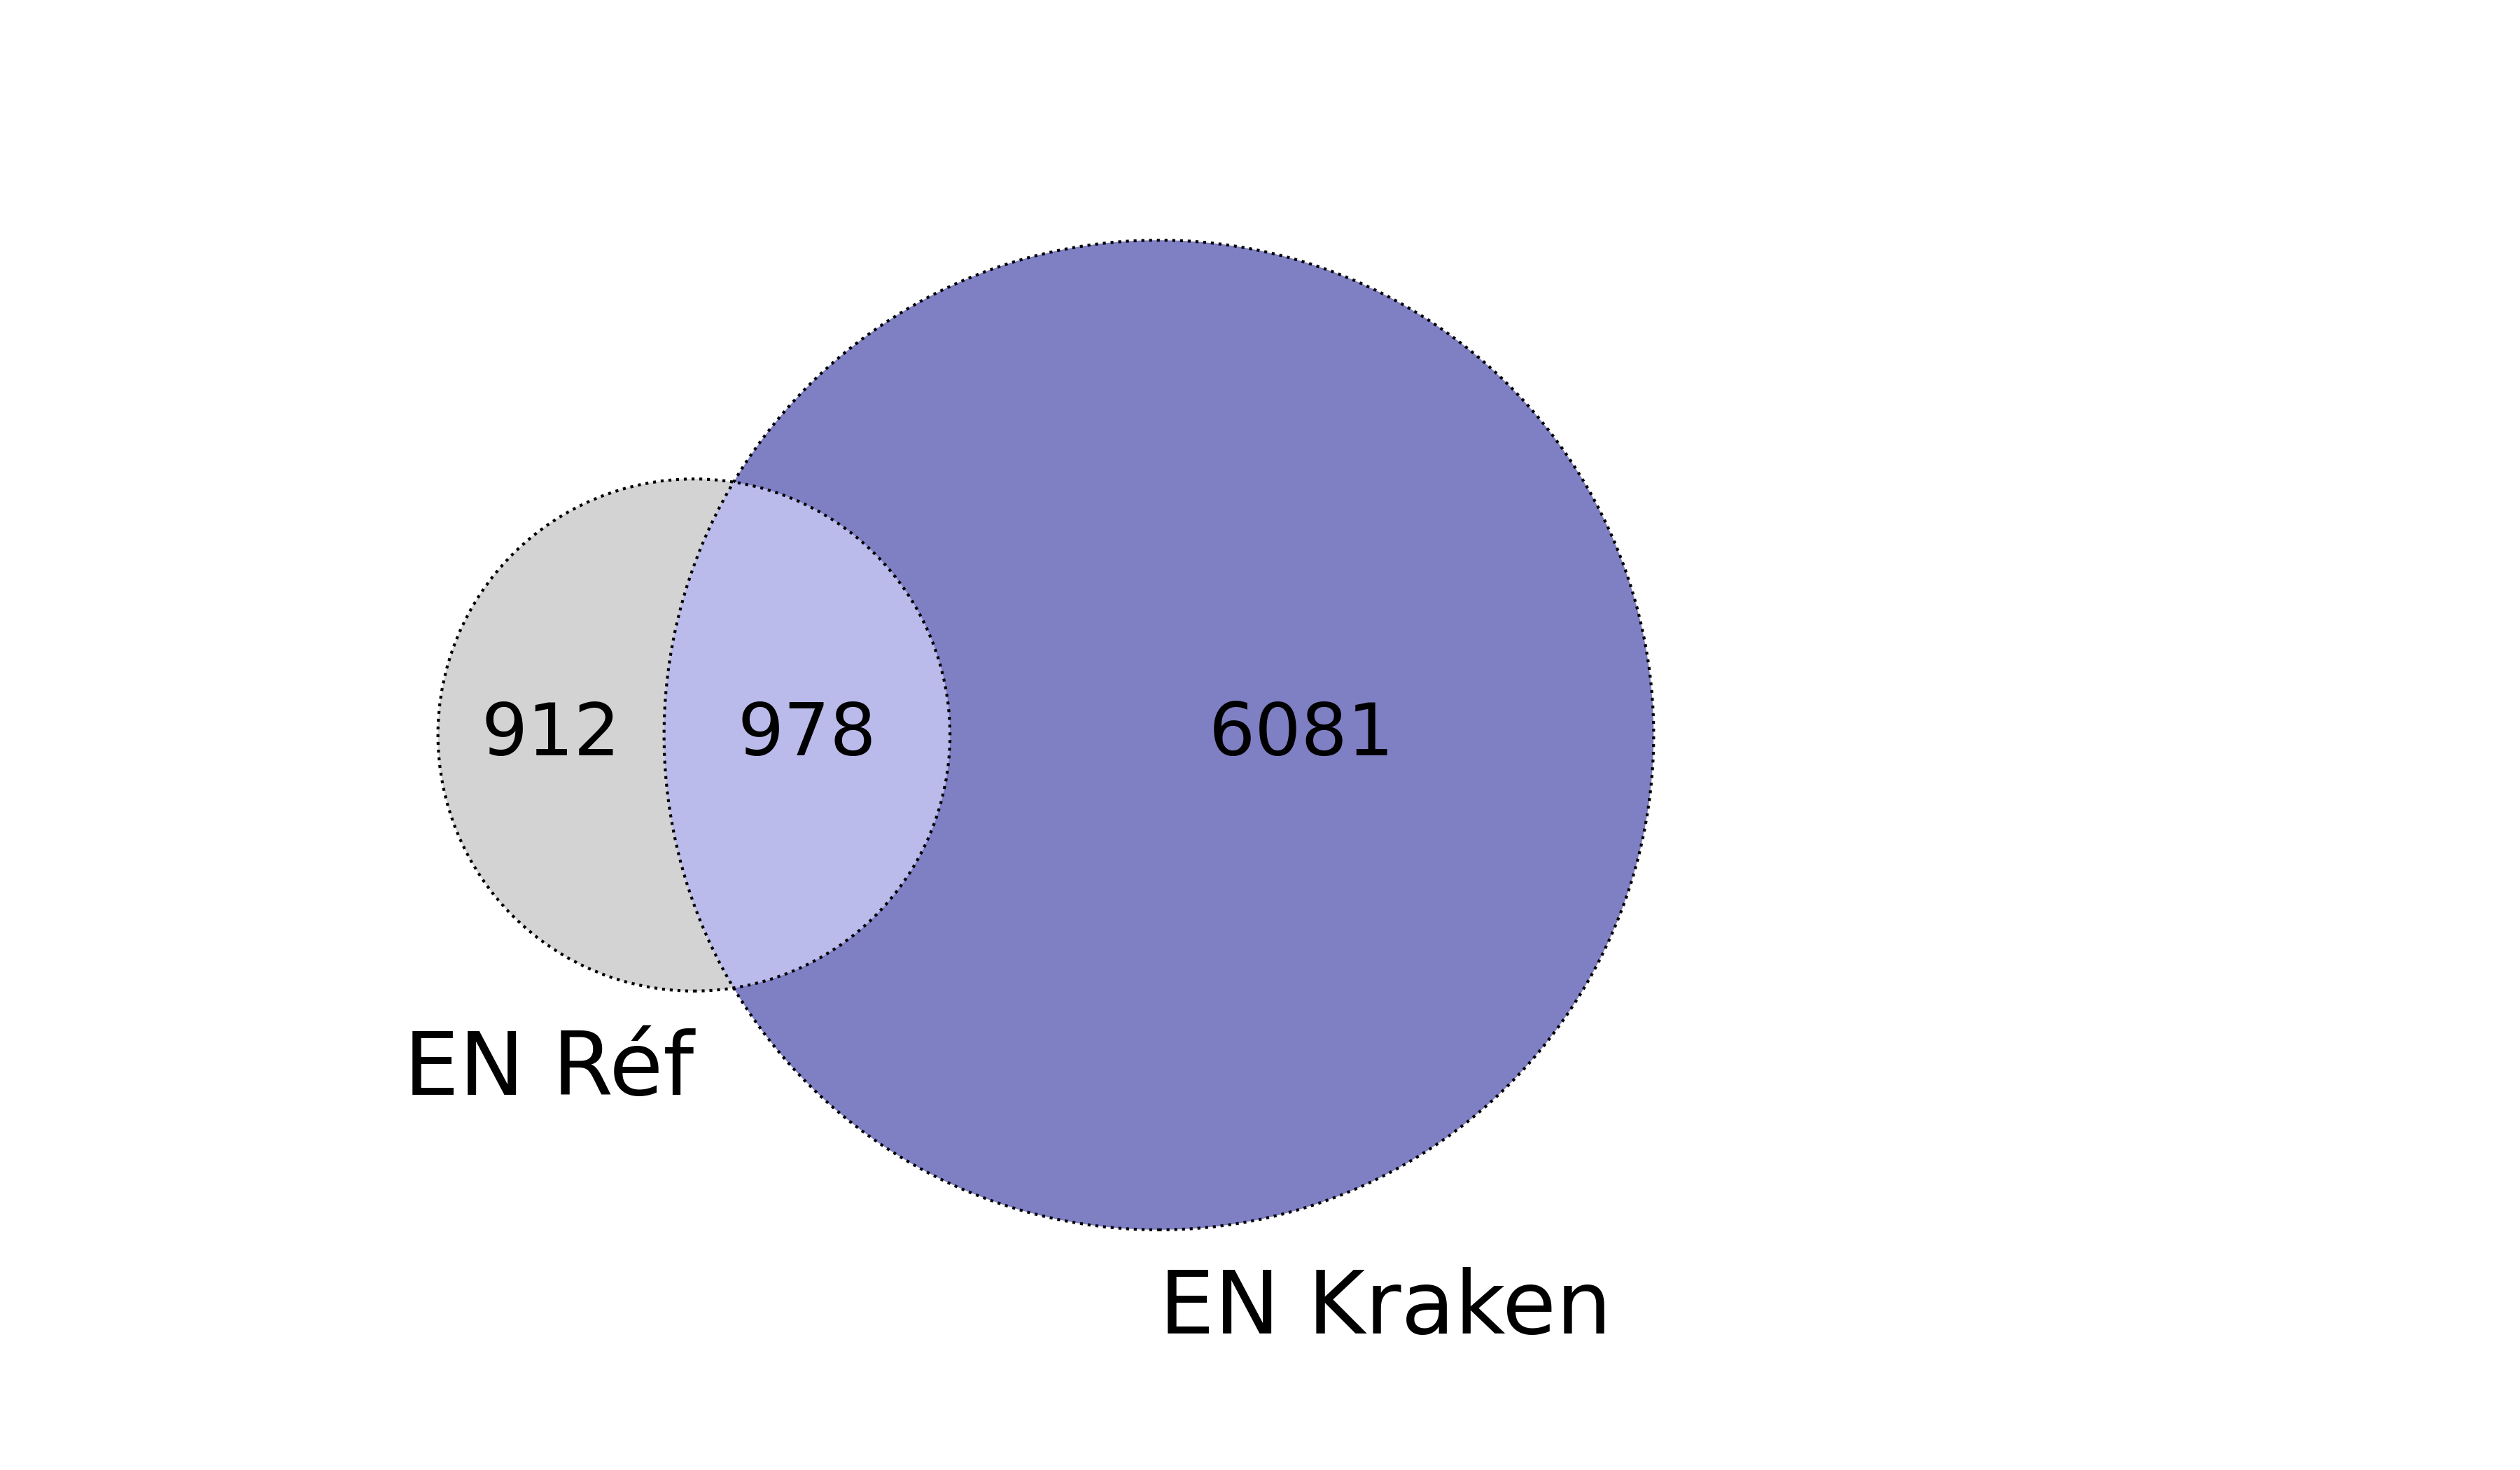
\includegraphics[width=1\textwidth]{IMAGES/INTERSECTIONS_GLOBALES/ELTeCFRA_Kraken_spacy-lg-concat_intersection.png} 
  \caption{Kraken --\texttt{spaCy-lg}}
  \label{fig:ELTeCFRA_Kraken_spacy-lg-concat_intersection}
  \end{subfigure}
  \end{minipage}
  \begin{minipage}{7cm}
  \begin{subfigure}{1\textwidth}
  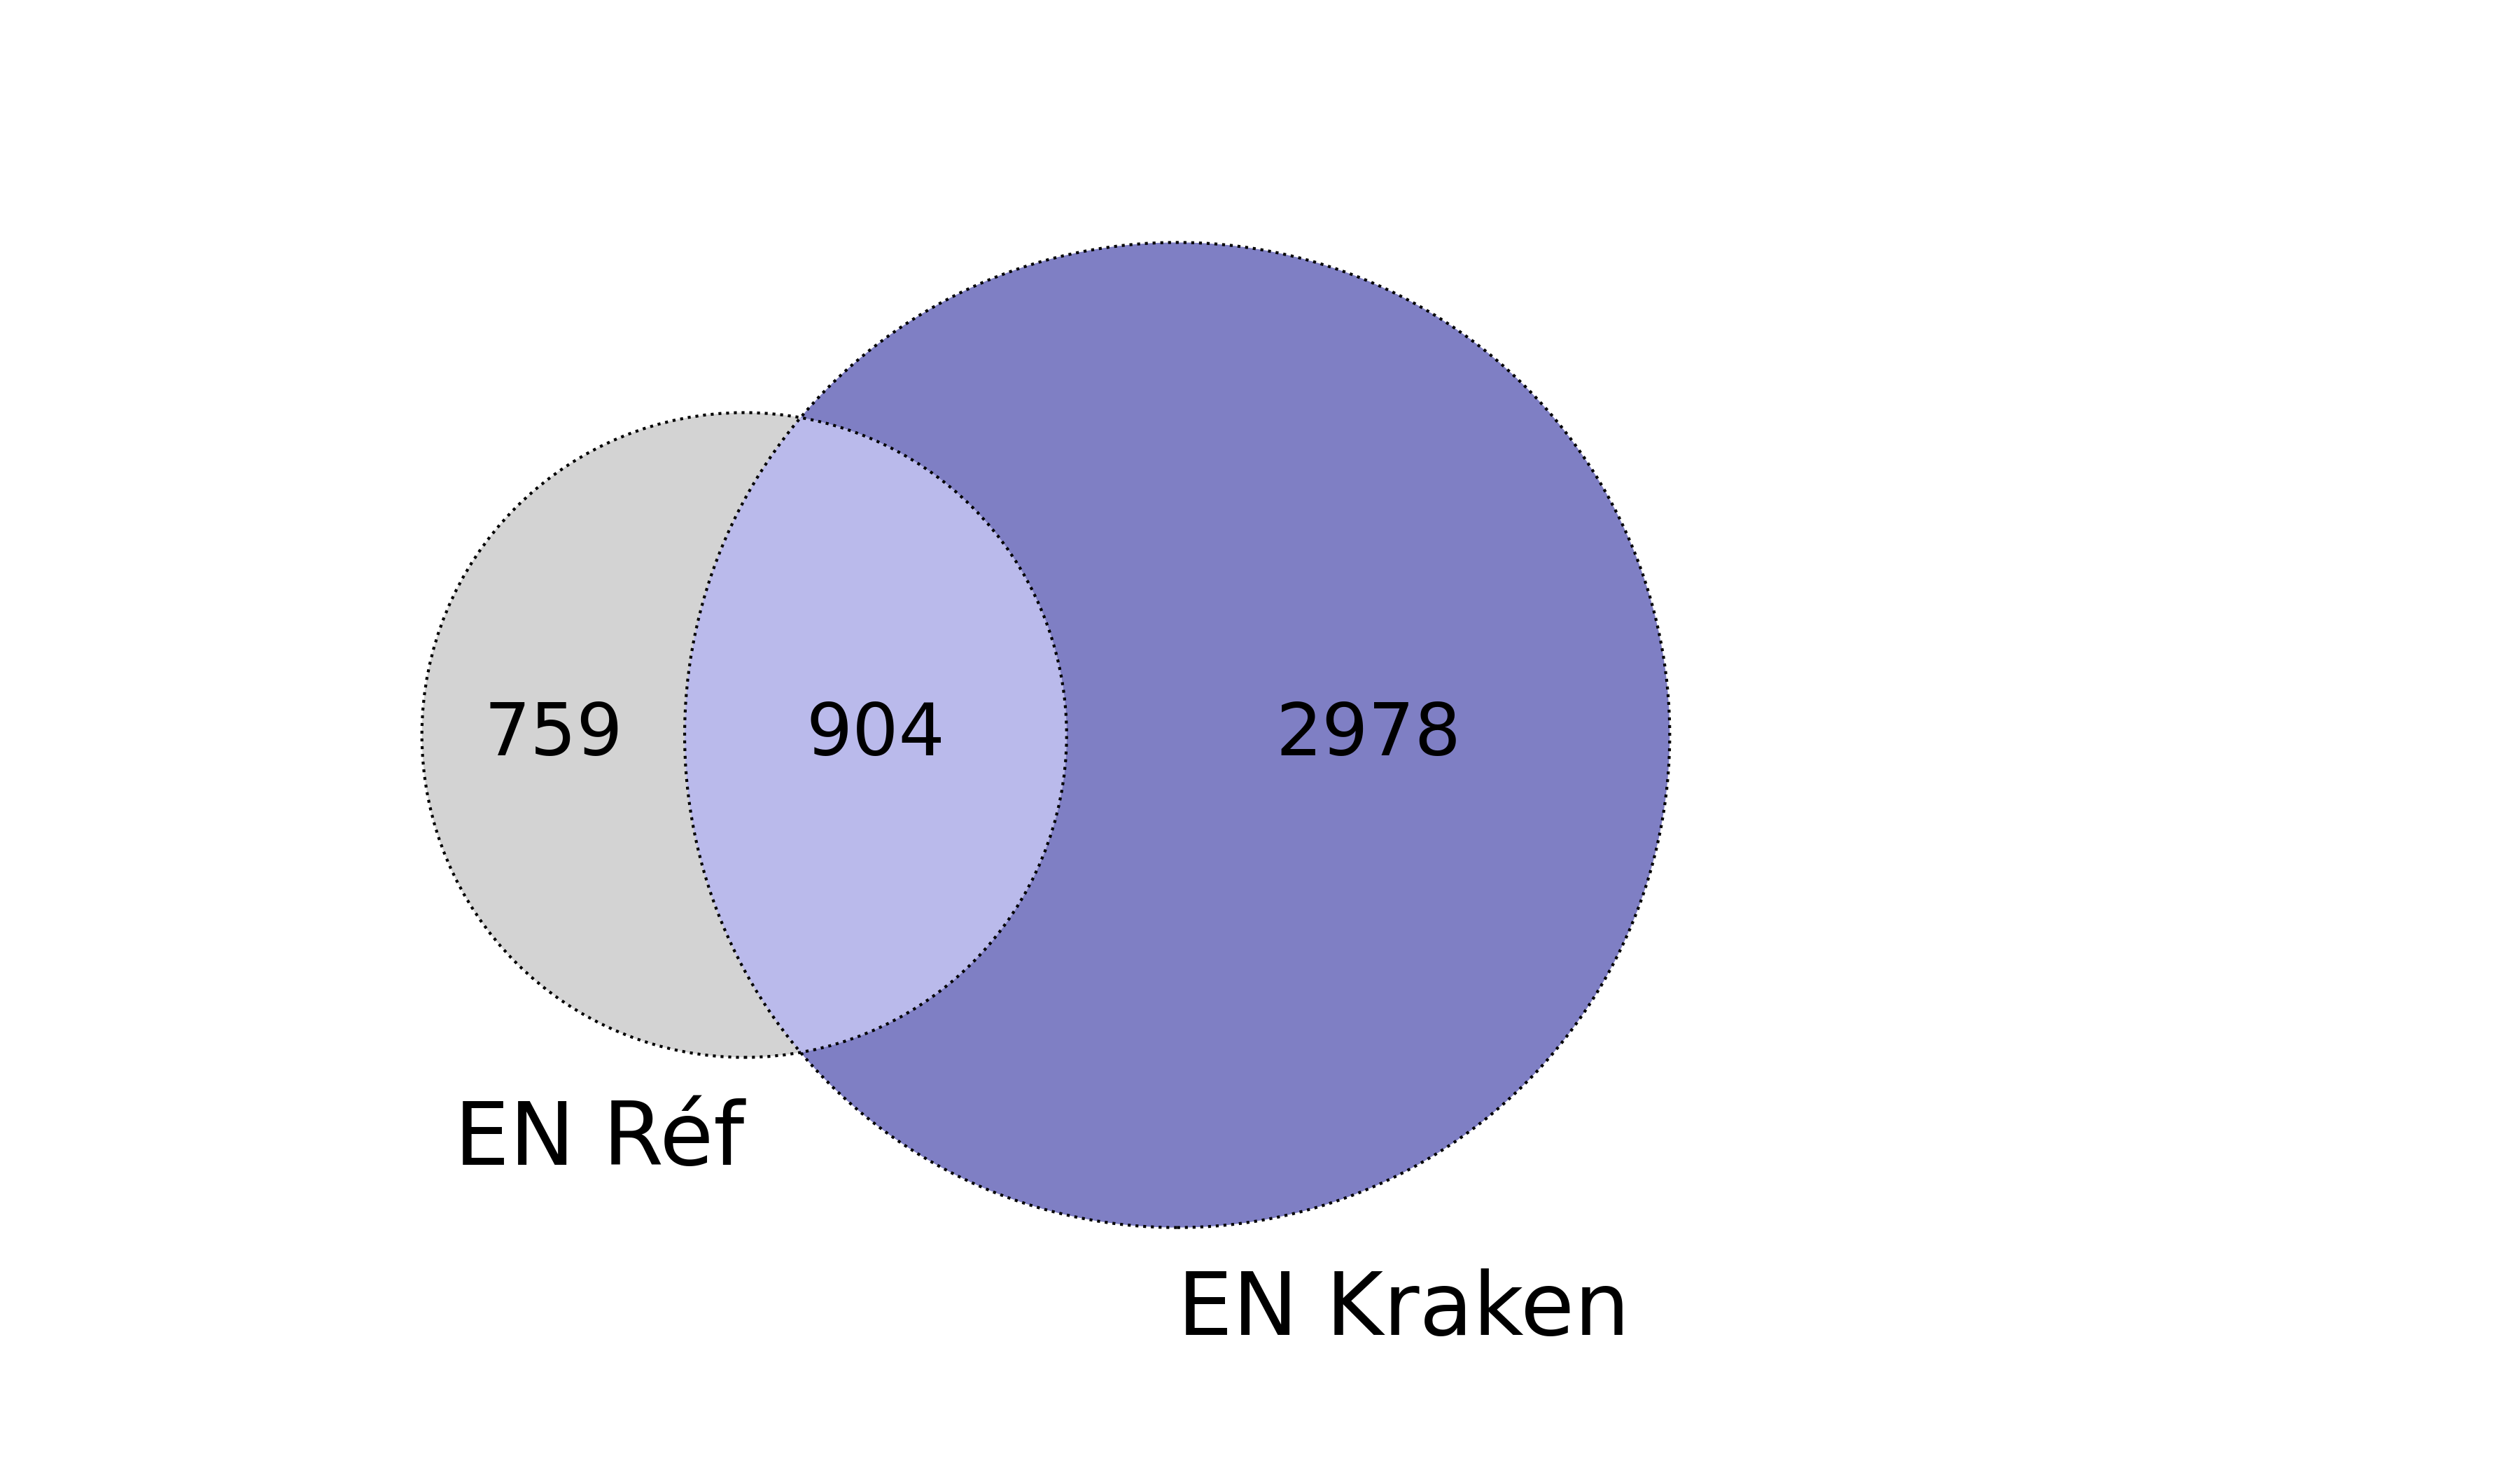
\includegraphics[width=1\textwidth]{IMAGES/INTERSECTIONS_GLOBALES/ELTeCFRA_Kraken_stanza-concat_intersection.png}
  \caption{Kraken -- \texttt{stanza}}
 % \label{fig:ELTeCFRA_Kraken_stanza-concat_intersection}
  \end{subfigure}
    \end{minipage}
\begin{minipage}{7cm}
  \begin{subfigure}{1\textwidth}
  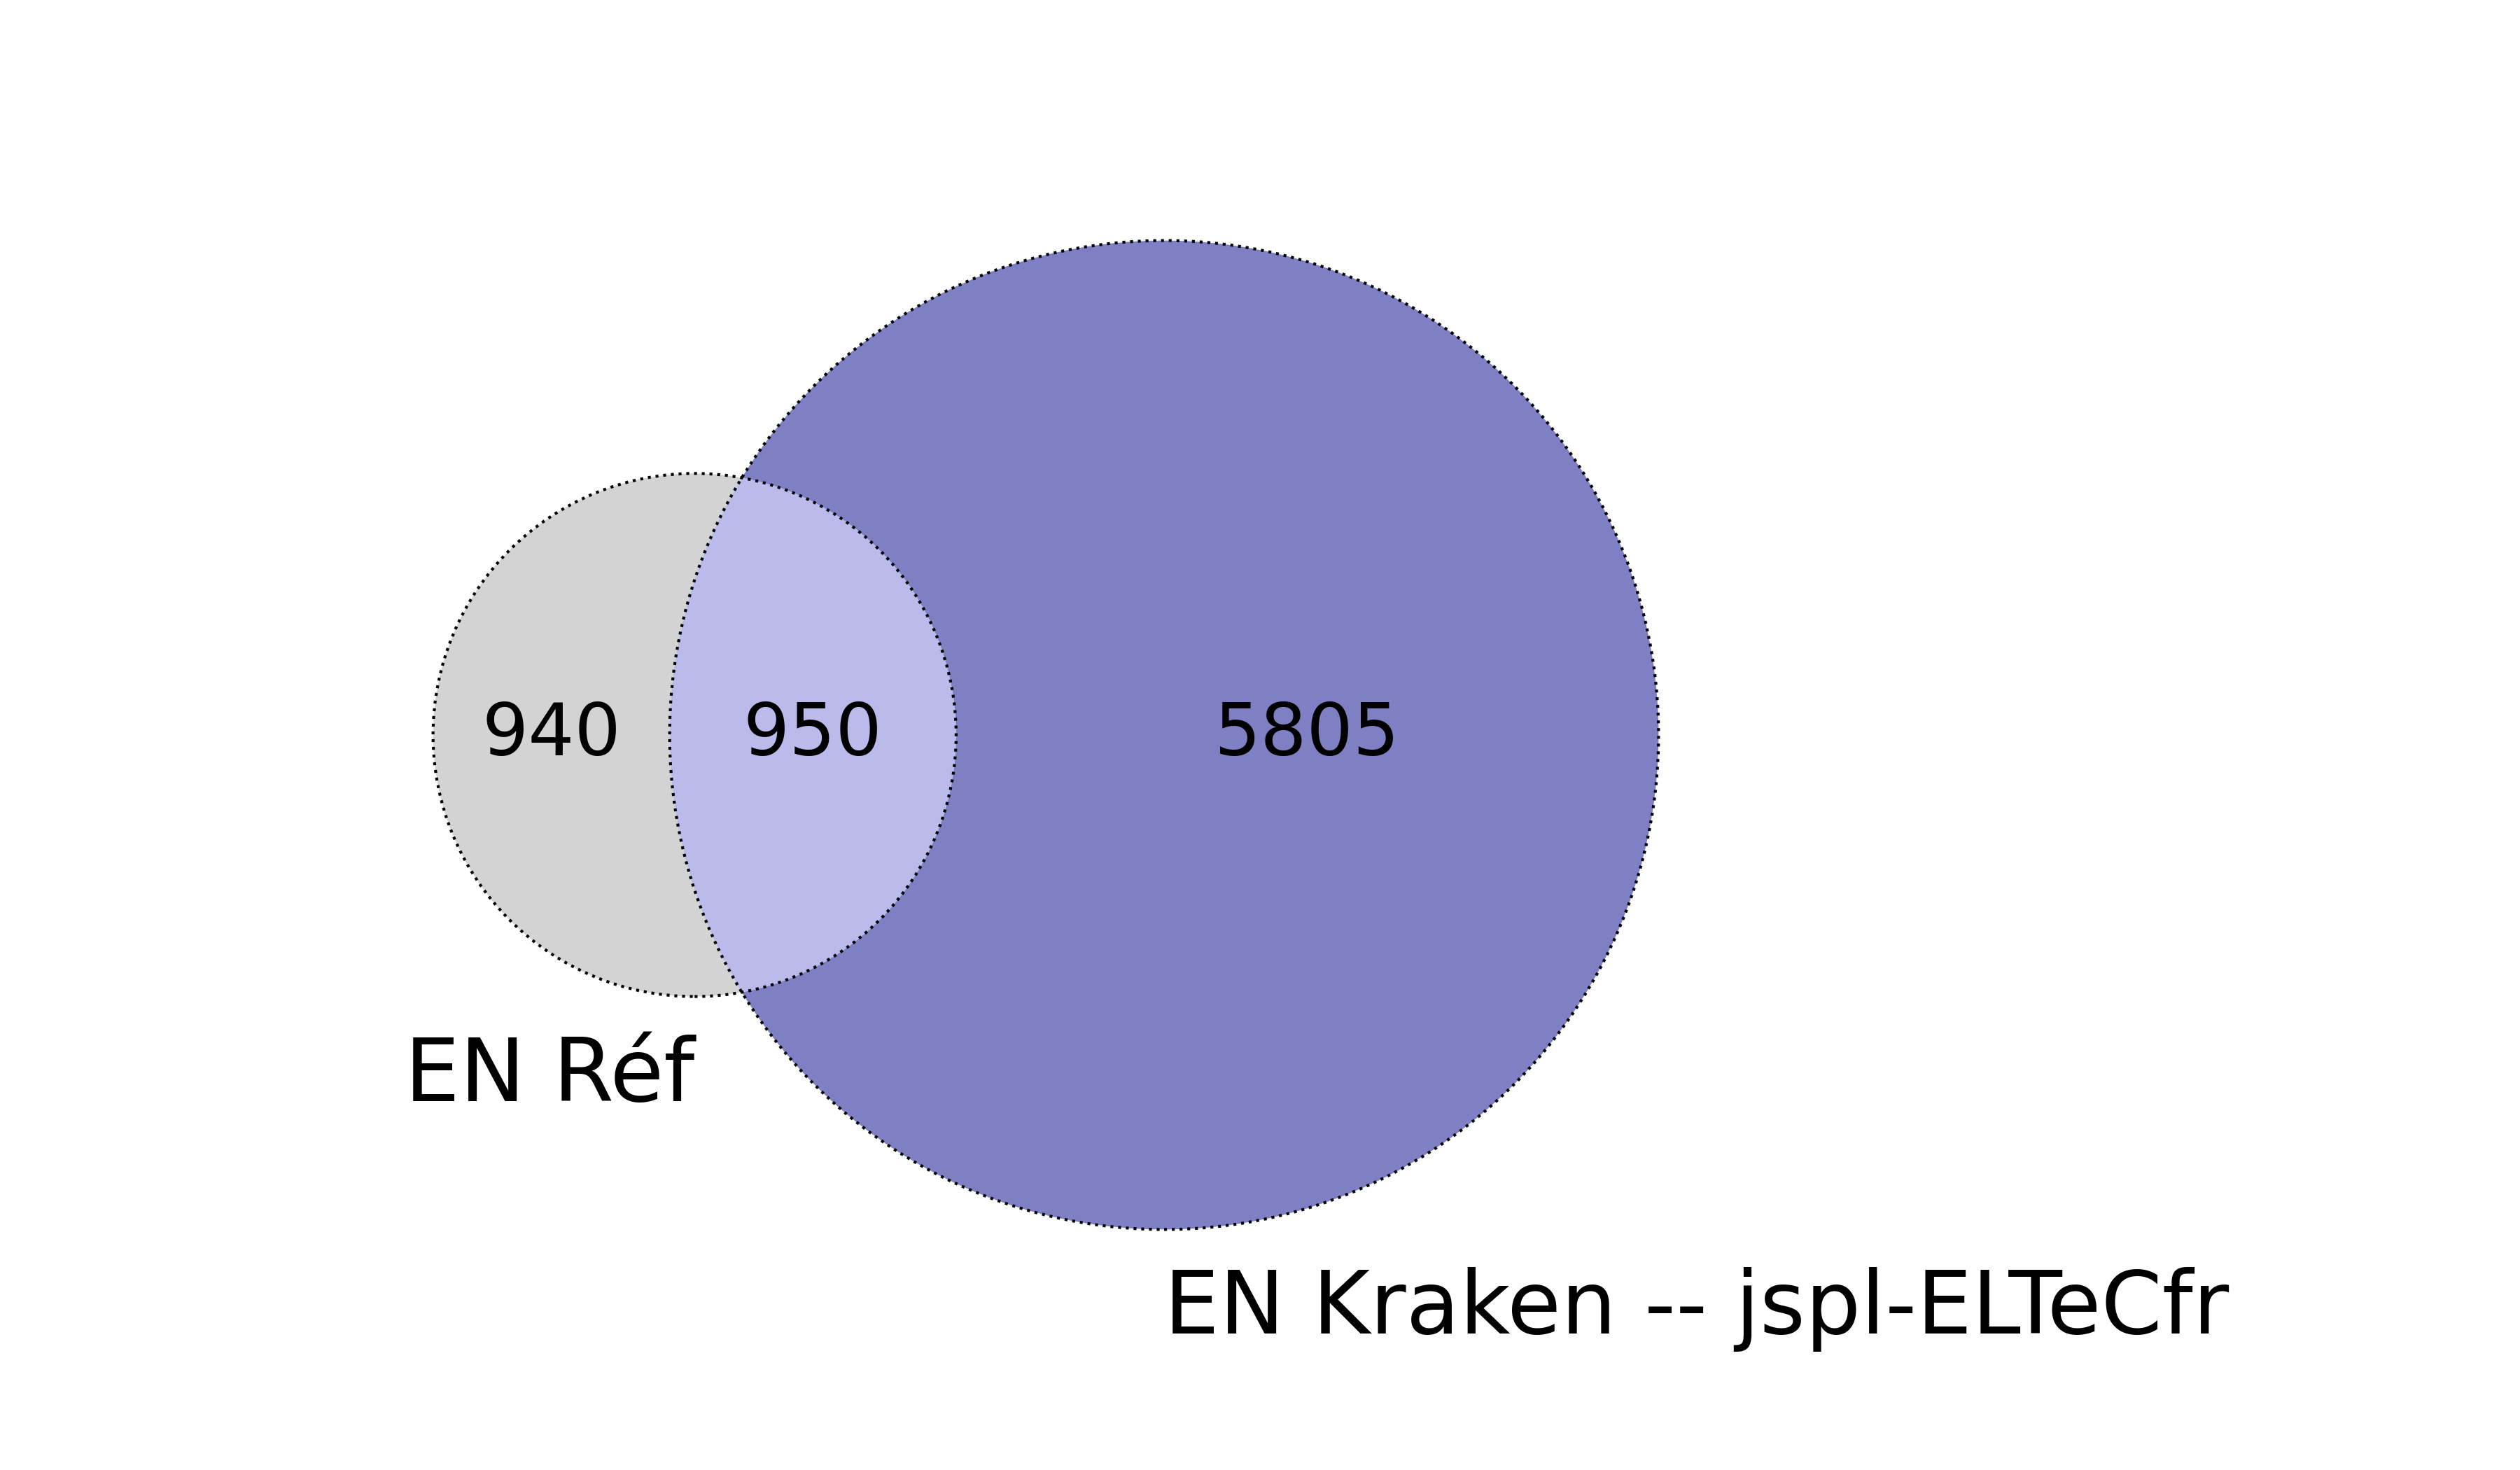
\includegraphics[width=1\textwidth]{IMAGES/INTERSECTIONS_GLOBALES/ELTeCFRA_Kraken -- jspl-ELTeCfr_spacy-lg-concat_intersection.png} 
  \caption{Kraken corrigé ELTeC-fr -- \texttt{spaCy-lg}}
  \label{fig:ELTeCFRA_Kraken -- jspl-ELTeCfr_spacy-lg-concat_intersection}
  \end{subfigure}
  \end{minipage}
  \begin{minipage}{7cm}
  \begin{subfigure}{1\textwidth}
  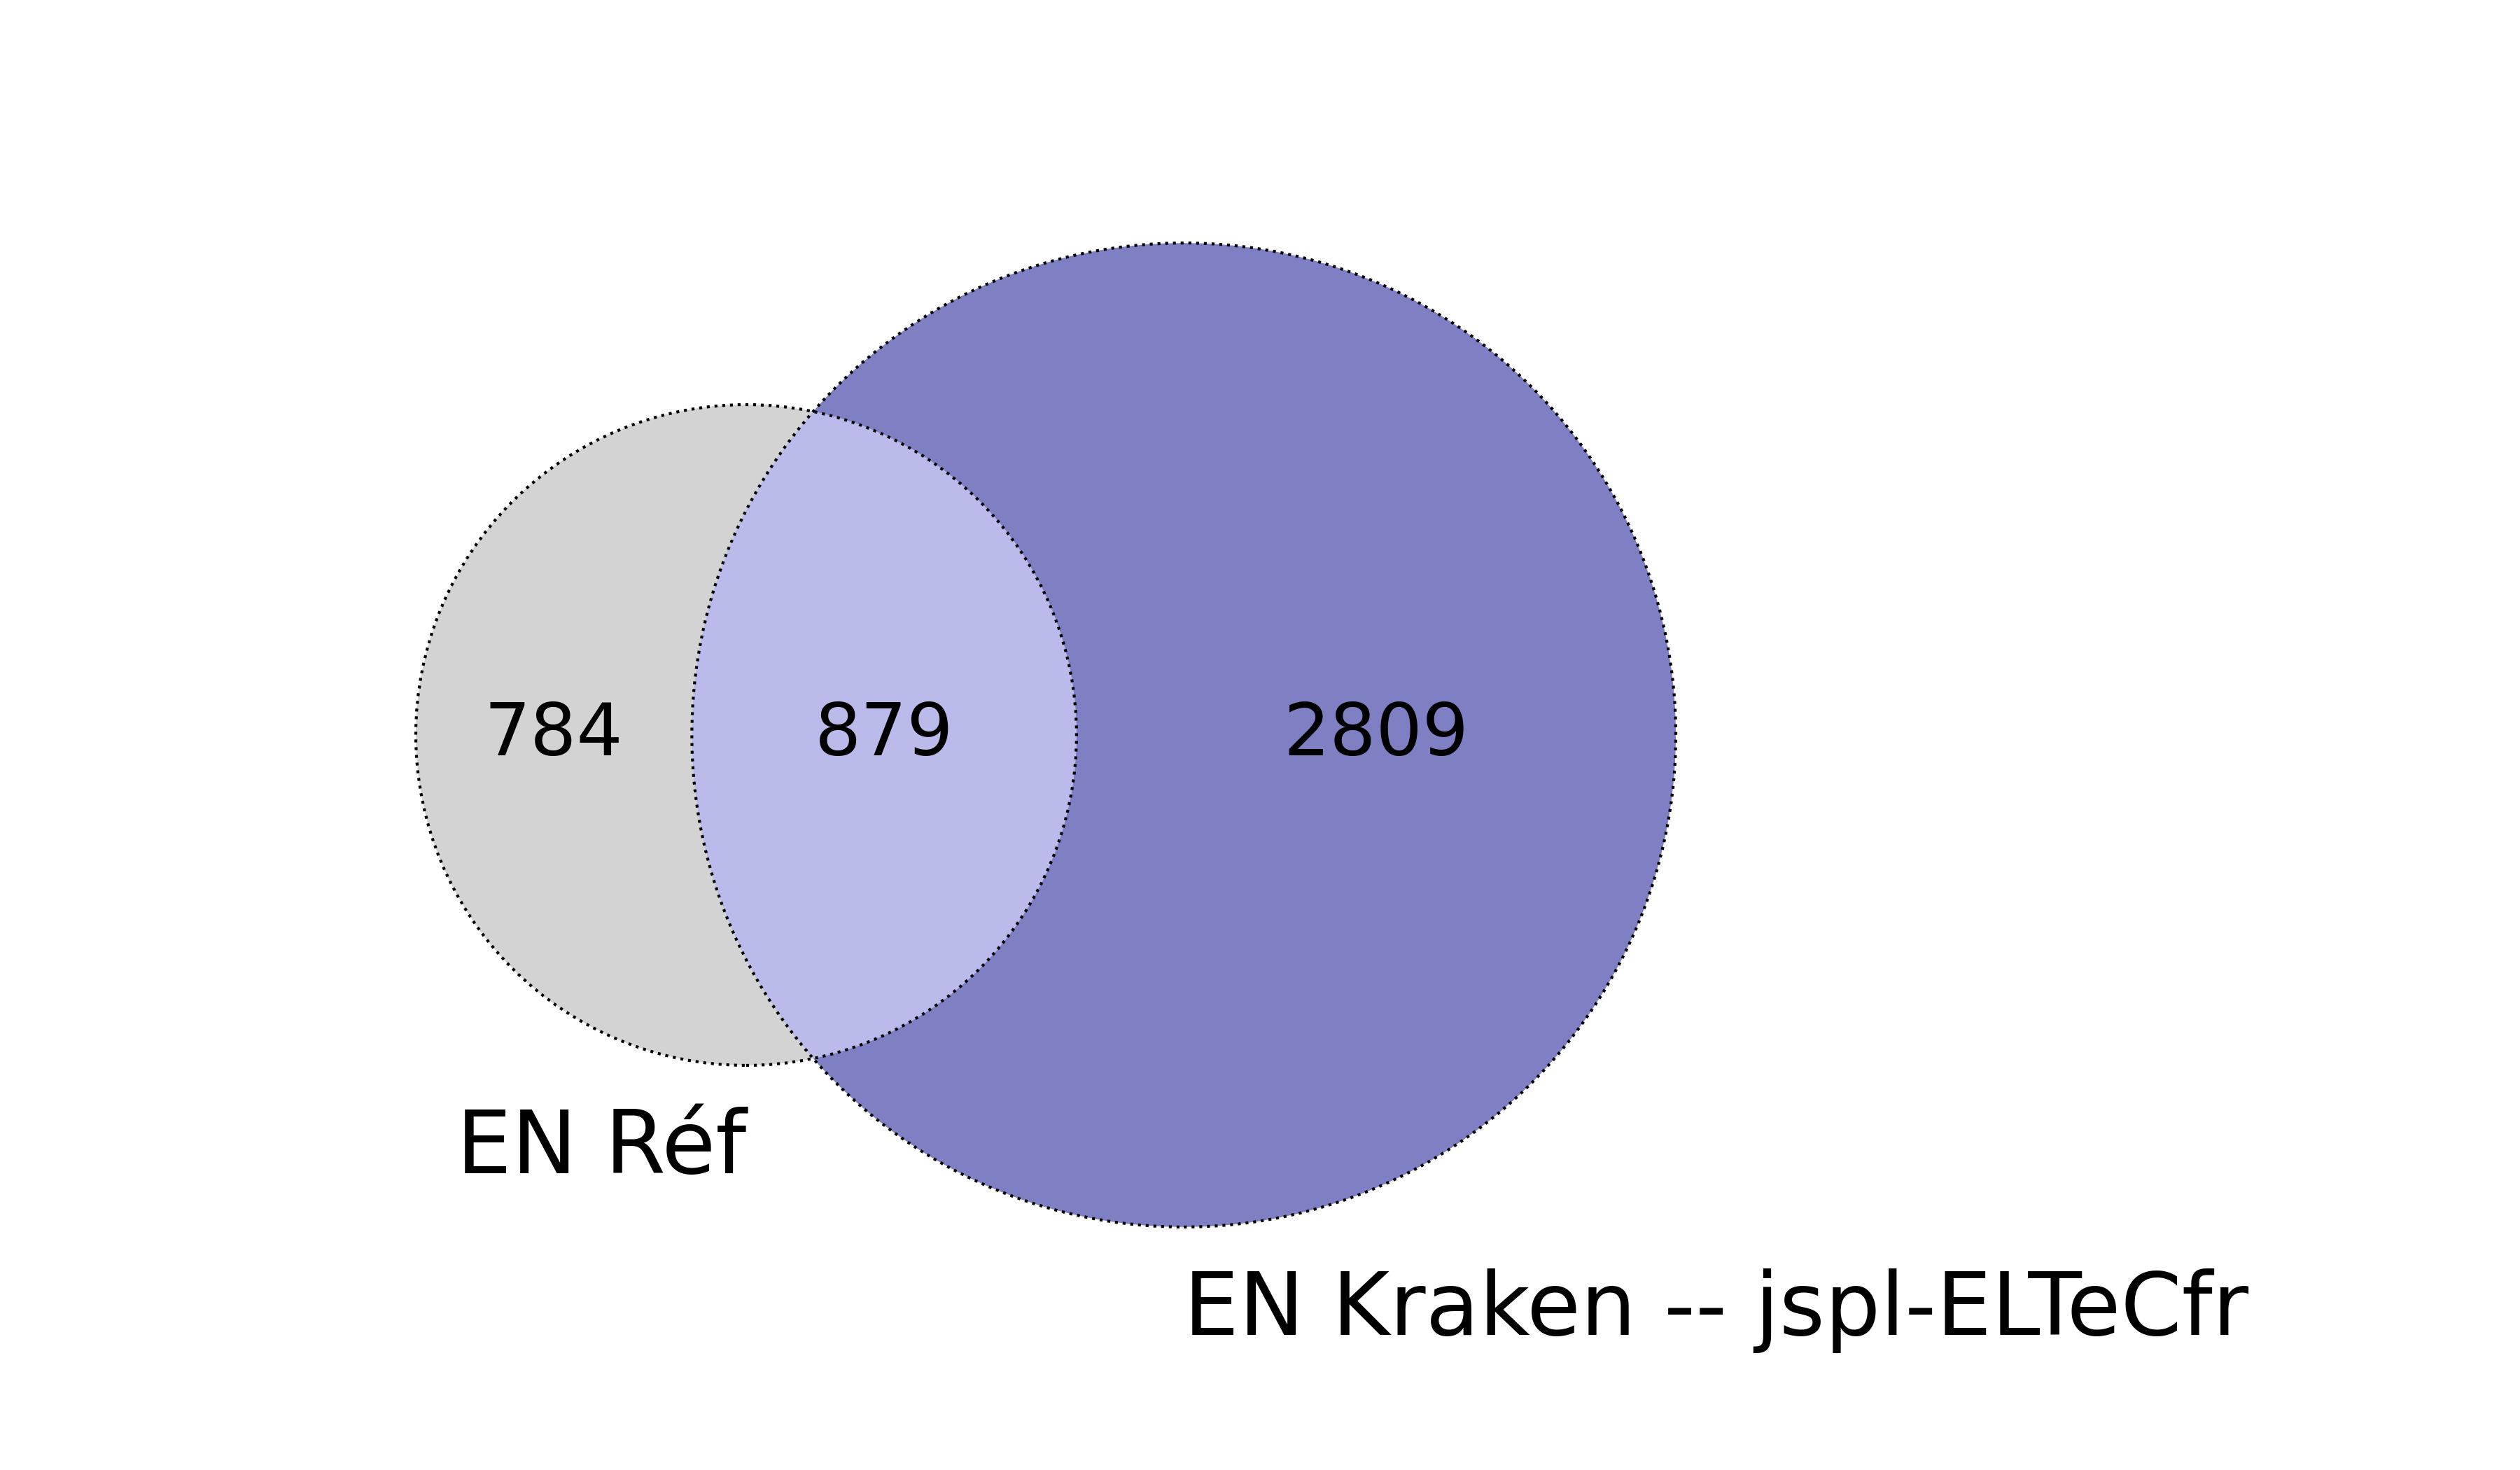
\includegraphics[width=1\textwidth]{IMAGES/INTERSECTIONS_GLOBALES/ELTeCFRA_Kraken -- jspl-ELTeCfr_stanza-concat_intersection.png}
  \caption{Kraken corrigé ELTeC-fr -- \texttt{stanza}}
  \label{fig:ELTeCFRA_Kraken -- jspl-ELTeCFR_stanza-concat_intersection}
  \end{subfigure}
    \end{minipage}
\caption{Intersections pour la configuration Kraken-\texttt{spaCy\_lg} corrigées avec JamSpell (modèle ELTeC), pour le sous-corpus ELTeC français.}
\label{fig:intersection_globale-kraken}
\end{figure}

Ce fait peut être lu à l'aune %- CKP : ne pas corriger cette expression : à l'aune veut dire : En considération de ; en mesurant par rapport à ; à la mesure de ; à la lumière de.
% LP : Oui, désolée, c'est moi qui ai fait une bêtise, je m'en suis rendue compte plus tard !!
des observations présentée dans le tableau \ref{tab:typologie_erreurs-corr_ELTeCEng} rapportant la typologie des erreurs de corrections. Autrement dit la correction automatique ne transforme pas toutes les EN contaminées par la ROC en EN corrigées strictement associables avec les EN du groupe de référence. Ainsi les BOIC (``Morlincourt'' qui devient ``Martincourt'') s'accumulant avec les EN contaminée MOI (``Morlincourtl'' qui reste ``Morlincourtl'') les résultats des intersections sont moins bons. Il semble qu'en moyenne pour les sous-corpus ELTeC français, anglais et portugais et celui de la TGB la correction automatique avec le modèle entraîné sur une partie de chaque sous-corpus ELTeC fasse perdre 5\% des EN dans l'intersection avec Kraken et 10\% avec Tesseract, concernant les modèles pré-entrainés on perd 3\% avec Kraken et 9\% avec Tesseract. Cette expérience est l'occasion des démontrer les limites d'une évaluation stricte de la REN sur des textes bruités et leurs versions corrigées. Il est notable que les contaminations de ROC d'une part et de la correction automatique d'autre part ne sont pas un frein à la REN, mais le sont bien pour l'évaluation de la qualité de la REN sur des données bruitées.

\begin{figure}[h!]
    \begin{minipage}{7cm}
  \begin{subfigure}{1\textwidth}
  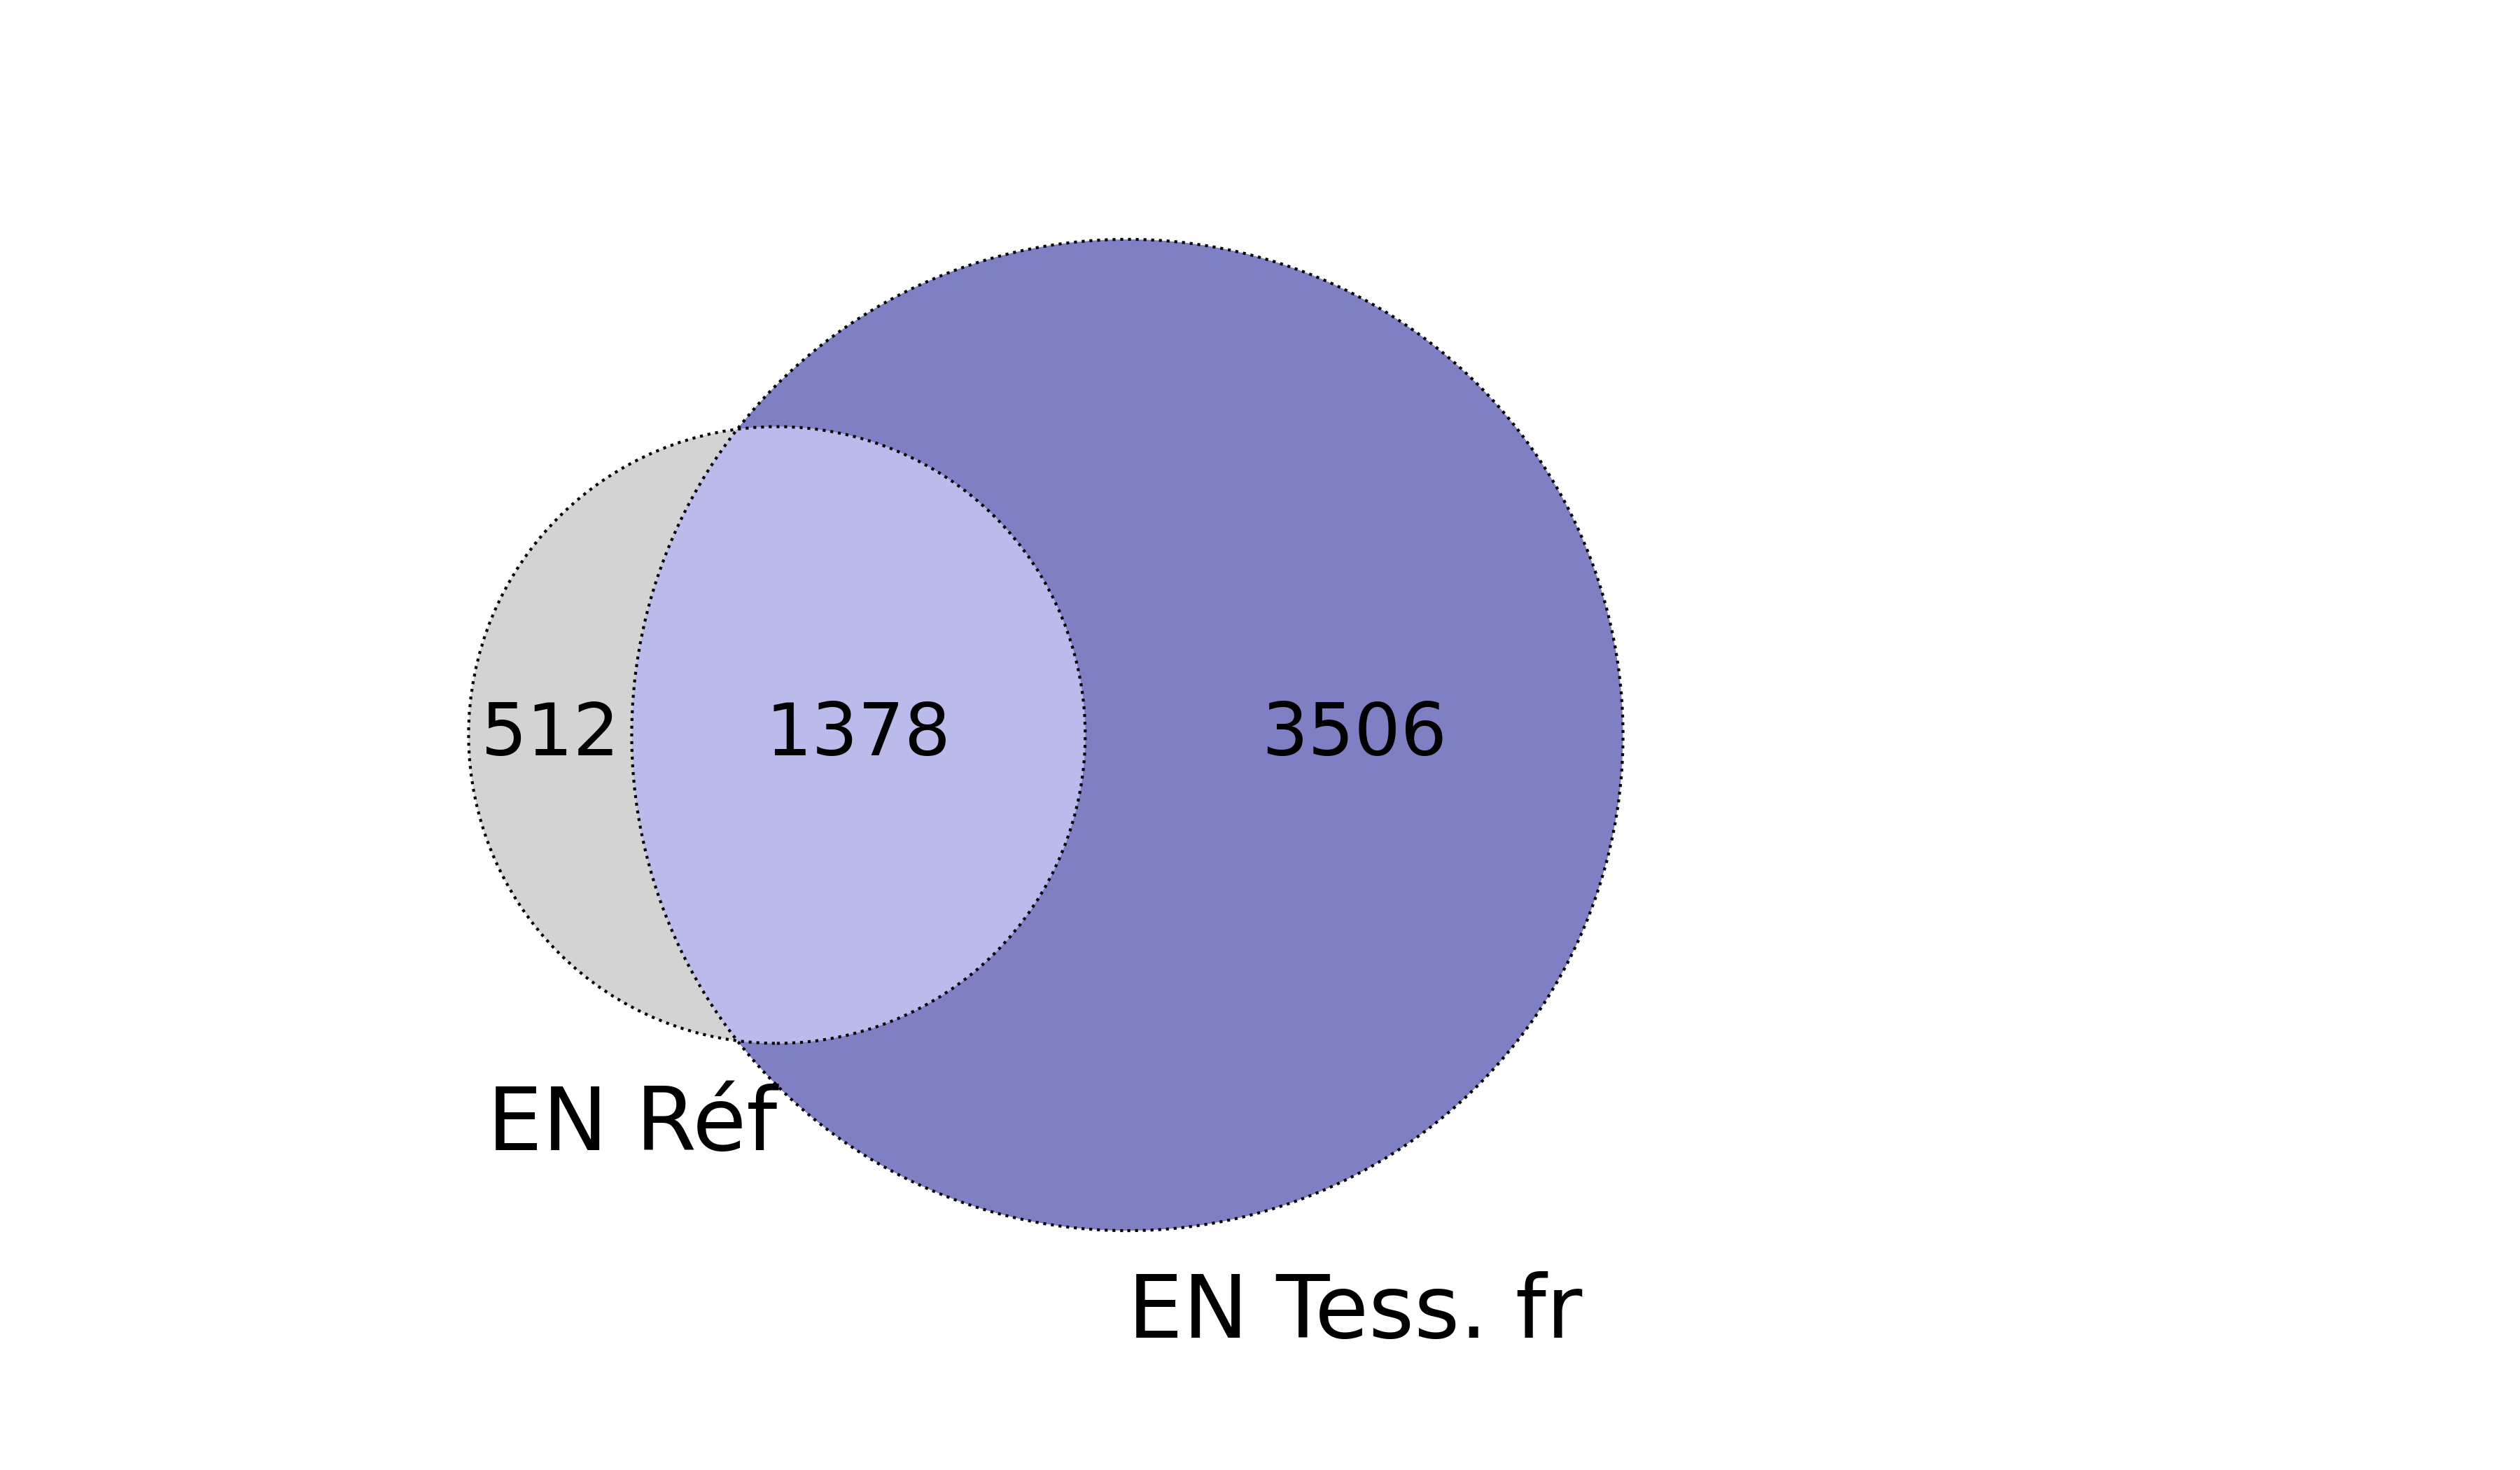
\includegraphics[width=1\textwidth]{IMAGES/INTERSECTIONS_GLOBALES/ELTeCFRA_Tess. fr_spacy-lg-concat_intersection.png} 
  \caption{Tess. fr. --\texttt{spaCy\_lg}}
  \label{fig:ELTeCFRA_Tess. fr_spacy-lg-concat_intersection}
  \end{subfigure}
  \end{minipage}
  \begin{minipage}{7cm}
  \begin{subfigure}{1\textwidth}
  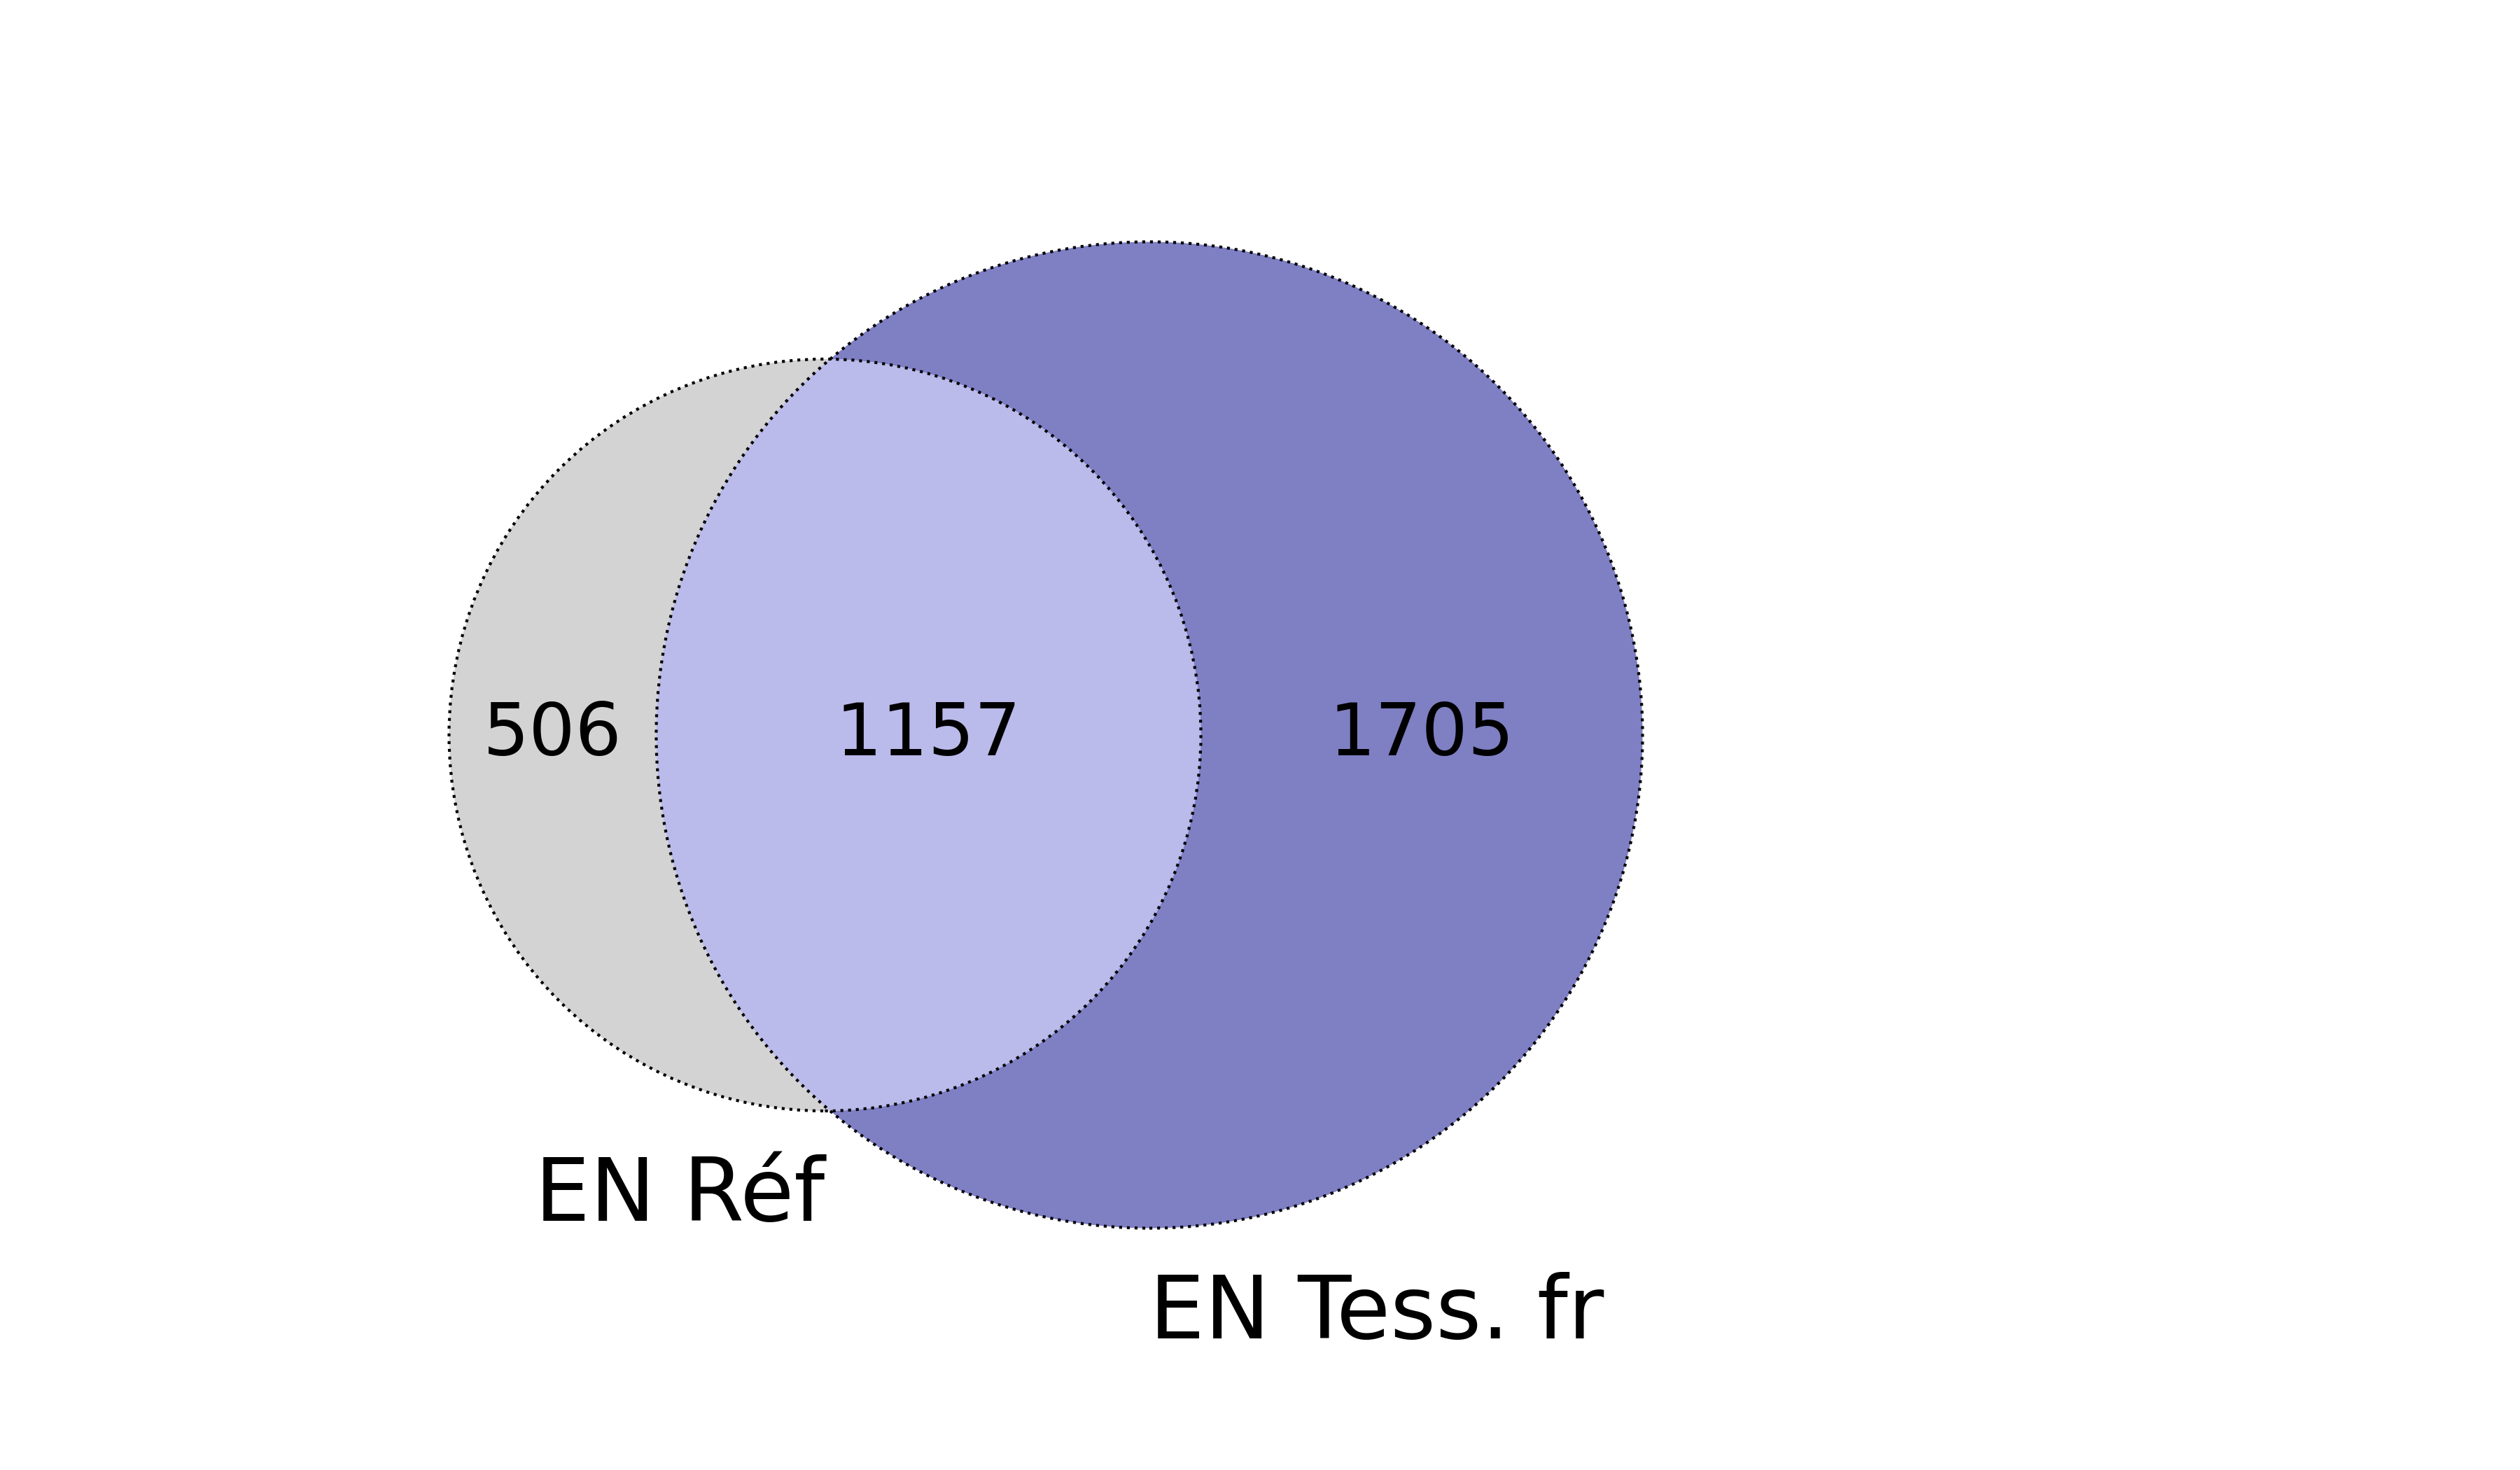
\includegraphics[width=1\textwidth]{IMAGES/INTERSECTIONS_GLOBALES/ELTeCFRA_Tess. fr_stanza-concat_intersection.png}
  \caption{Tess. fr. -- \texttt{stanza}}
 % \label{fig:ELTeCFRA_Tess. fr_stanza-concat_intersection}
  \end{subfigure}
    \end{minipage}
\begin{minipage}{7cm}
  \begin{subfigure}{1\textwidth}
  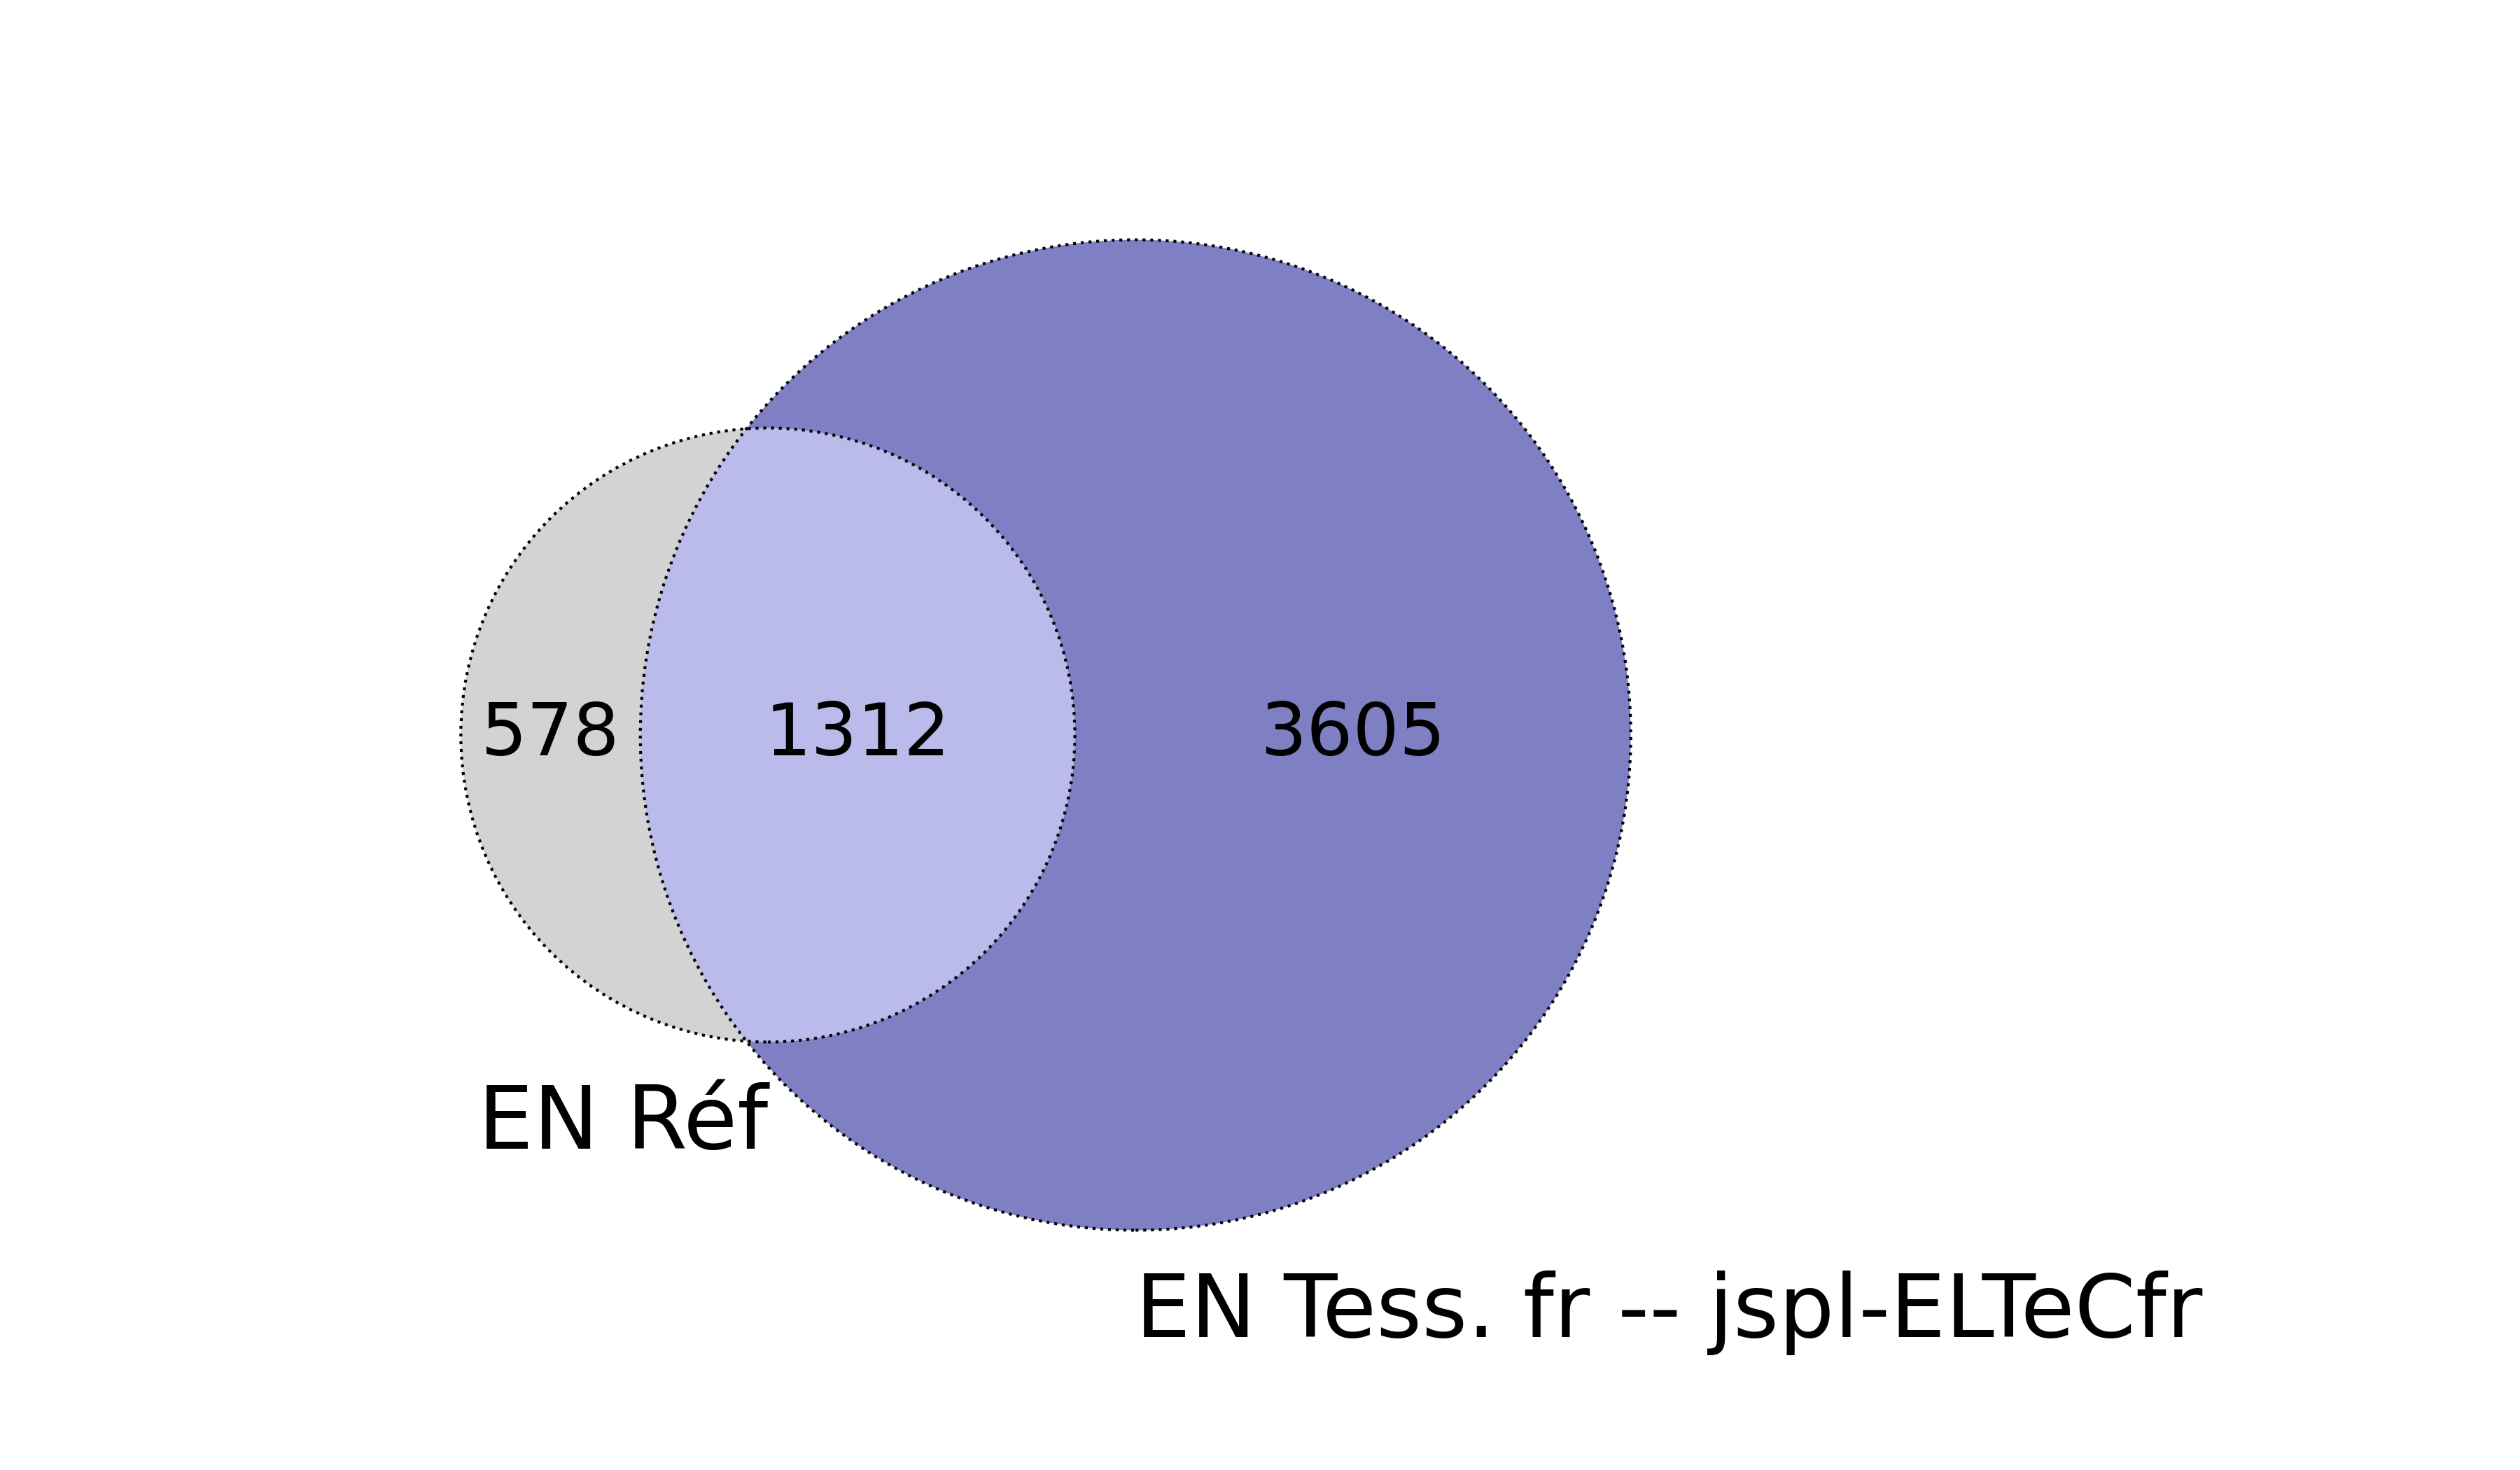
\includegraphics[width=1\textwidth]{IMAGES/INTERSECTIONS_GLOBALES/ELTeCFRA_Tess. fr -- jspl-ELTeCfr_spacy-lg-concat_intersection.png} 
  \caption{Tess. fr. corrigé -- \texttt{spaCy\_lg}}
  \label{fig:ELTeCFRA_Tess. fr -- jspl-ELTeCfr_spacy-lg-concat_intersection}
  \end{subfigure}
  \end{minipage}
  \begin{minipage}{7cm}
  \begin{subfigure}{1\textwidth}
  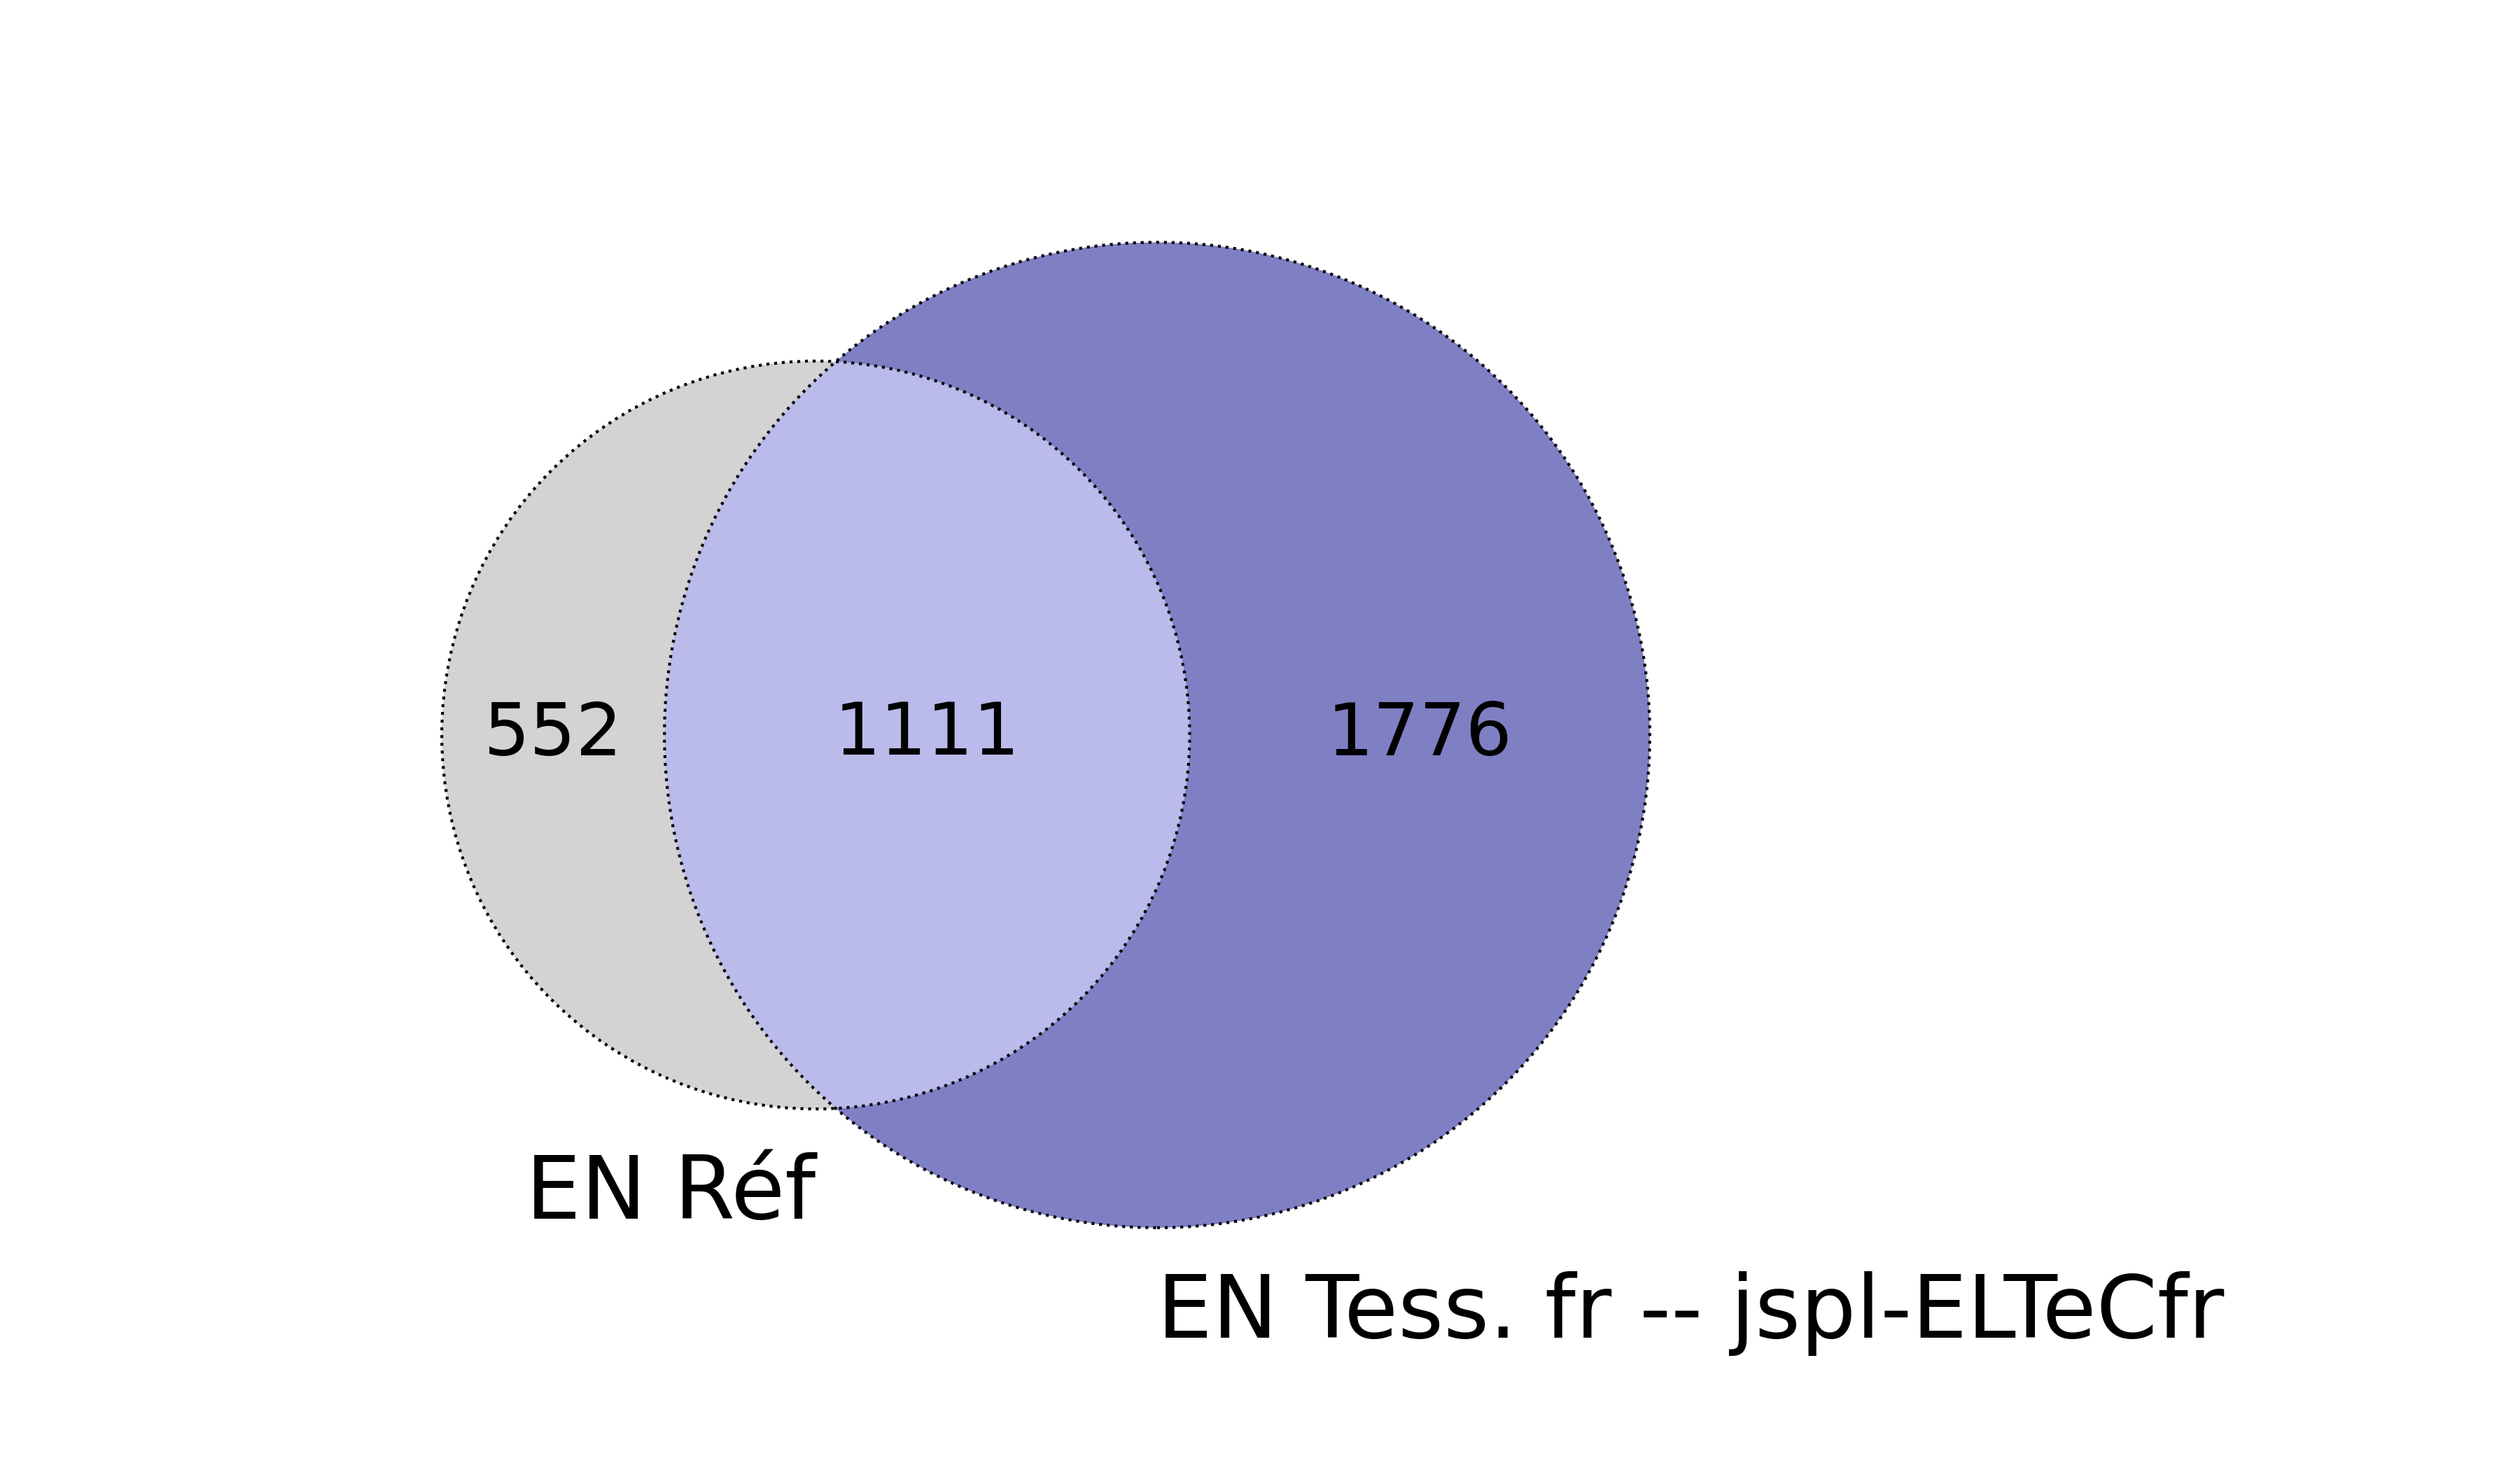
\includegraphics[width=1\textwidth]{IMAGES/INTERSECTIONS_GLOBALES/ELTeCFRA_Tess. fr -- jspl-ELTeCfr_stanza-concat_intersection.png}
  \caption{Tess. fr. corrigé -- \texttt{stanza}}
  \label{fig:ELTeCFRA_Tess. fr -- jspl-ELTeCfr_stanza-concat_intersection}
  \end{subfigure}
    \end{minipage}
\begin{minipage}{7cm}
  \begin{subfigure}{1\textwidth}
  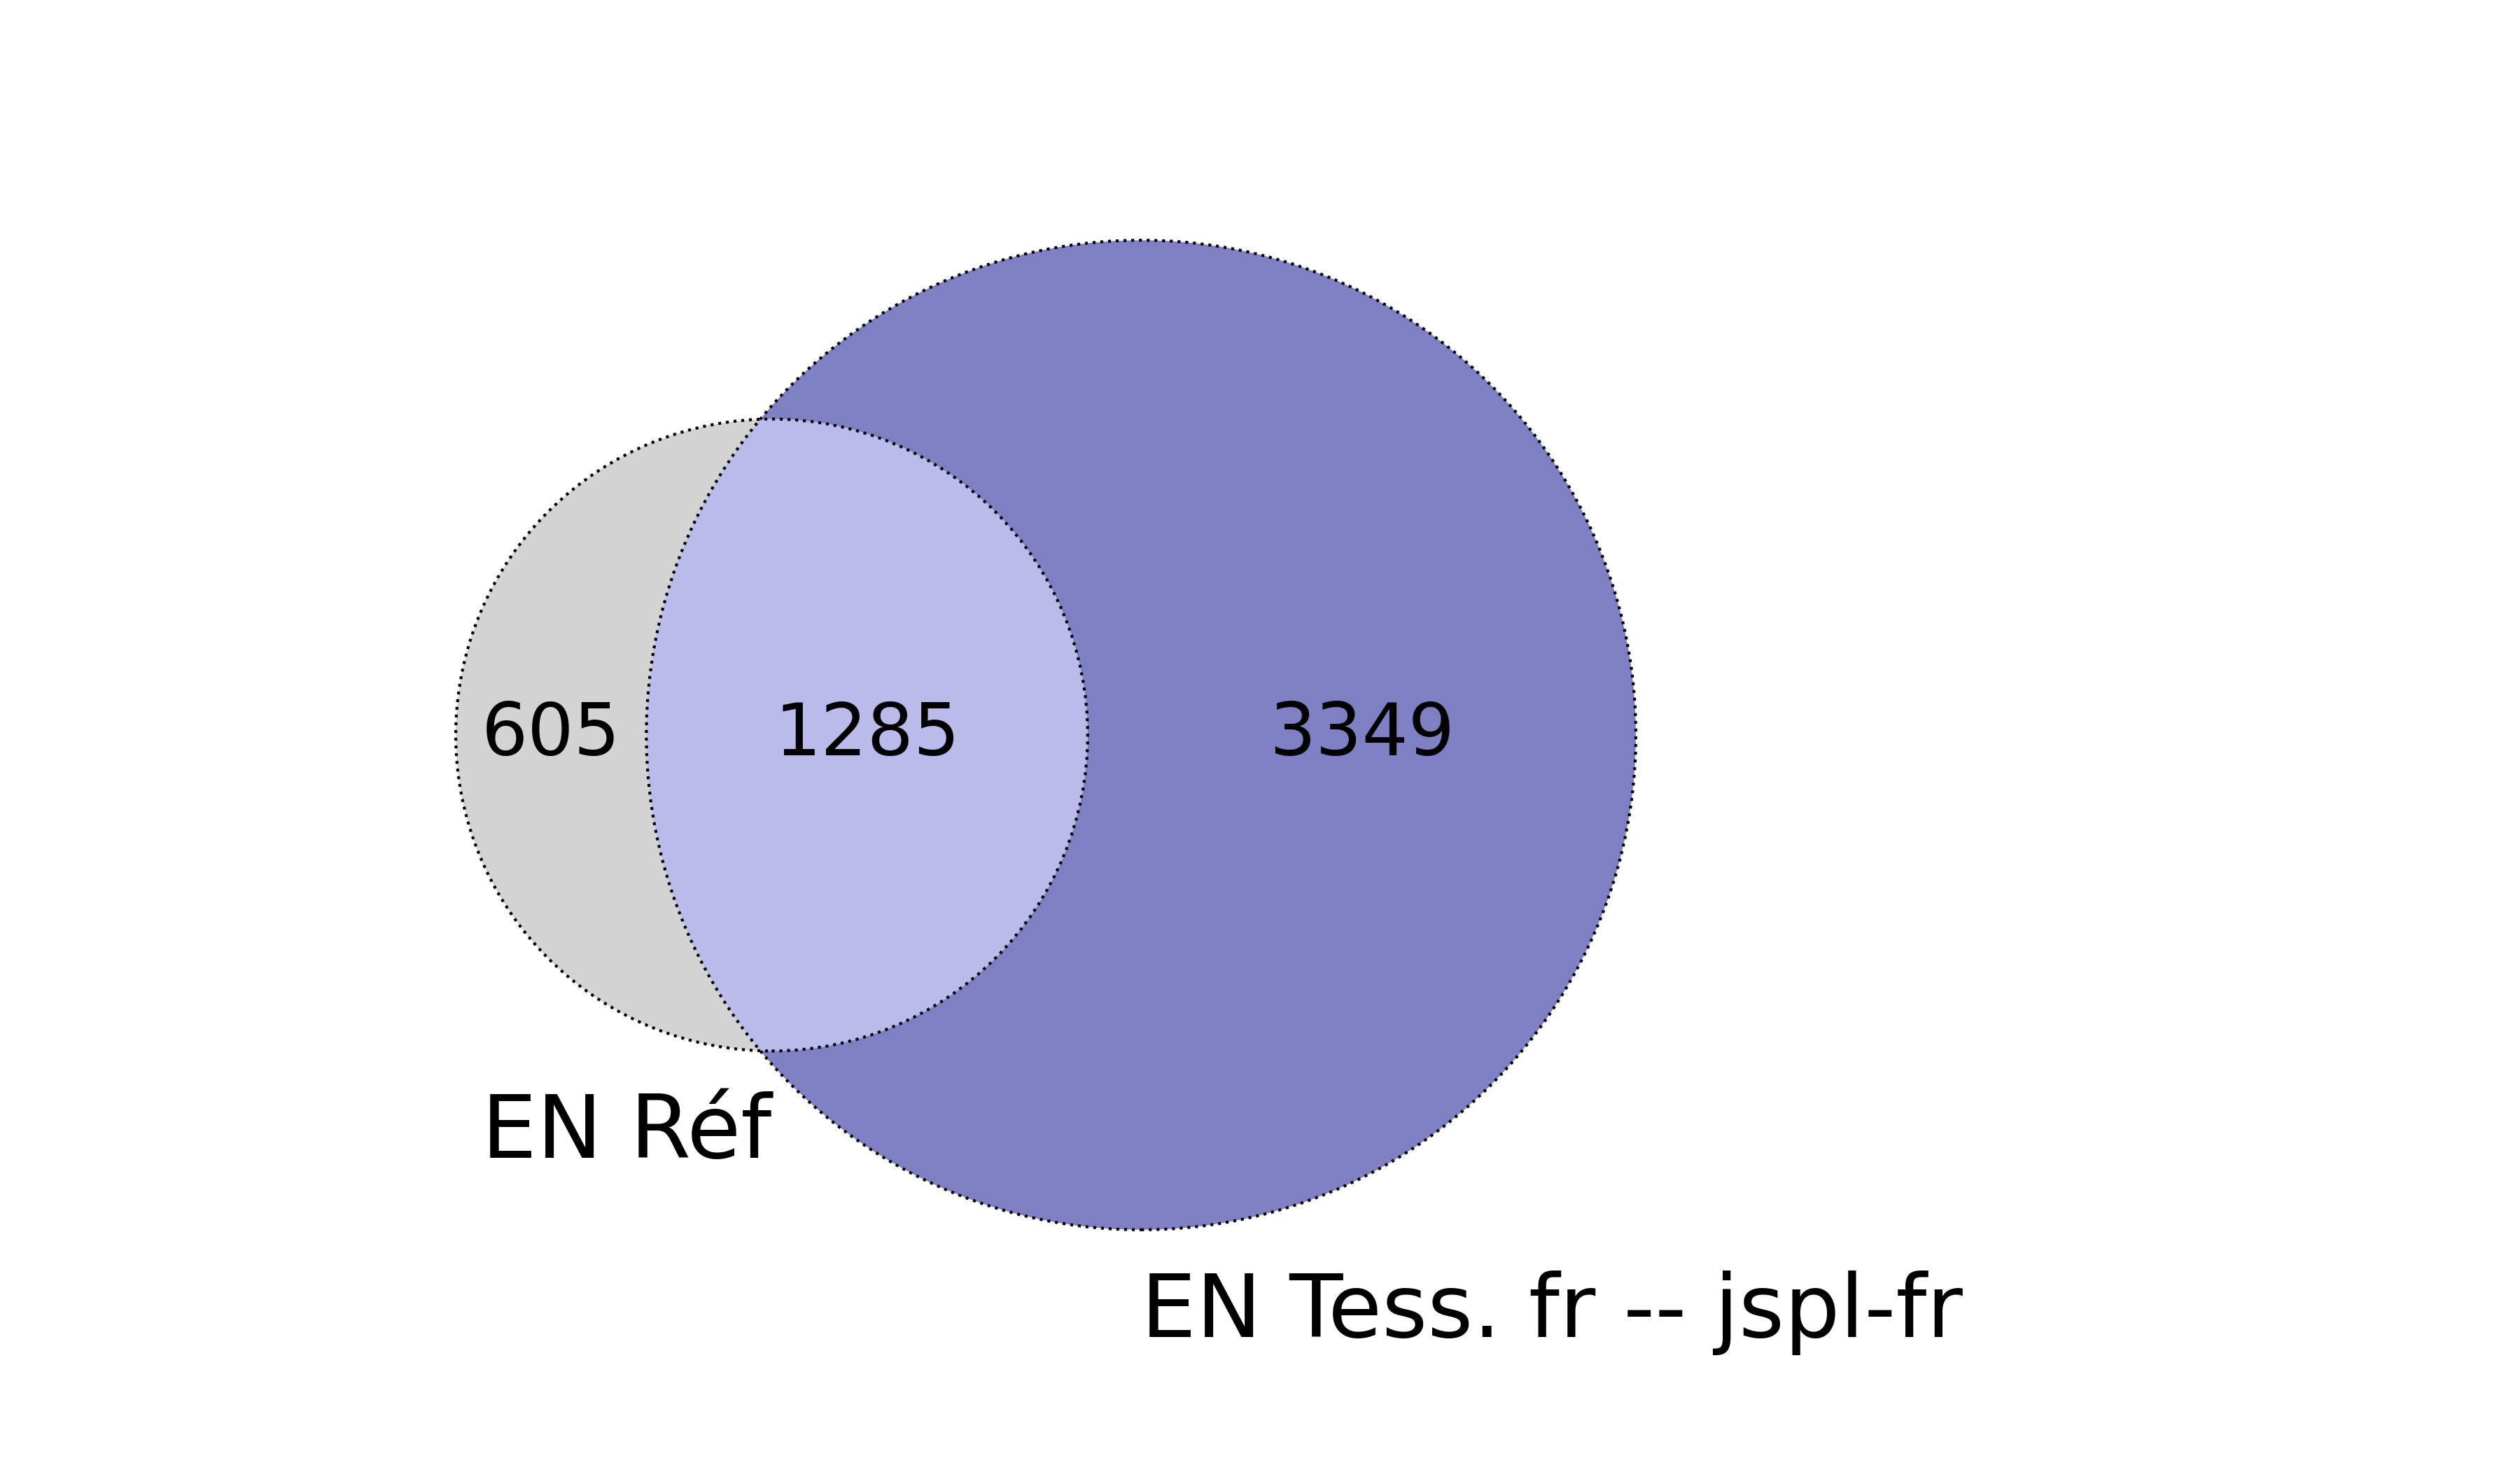
\includegraphics[width=1\textwidth]{IMAGES/INTERSECTIONS_GLOBALES/ELTeCFRA_Tess. fr -- jspl-fr_spacy-lg-concat_intersection.png} 
  \caption{Tess. fr. corrigé -- \texttt{spaCy\_lg}}
  \label{fig:ELTeCFRA_Tess. fr -- jspl-fr_spacy-lg-concat_intersection}
  \end{subfigure}
  \end{minipage}
  \begin{minipage}{7cm}
  \begin{subfigure}{1\textwidth}
  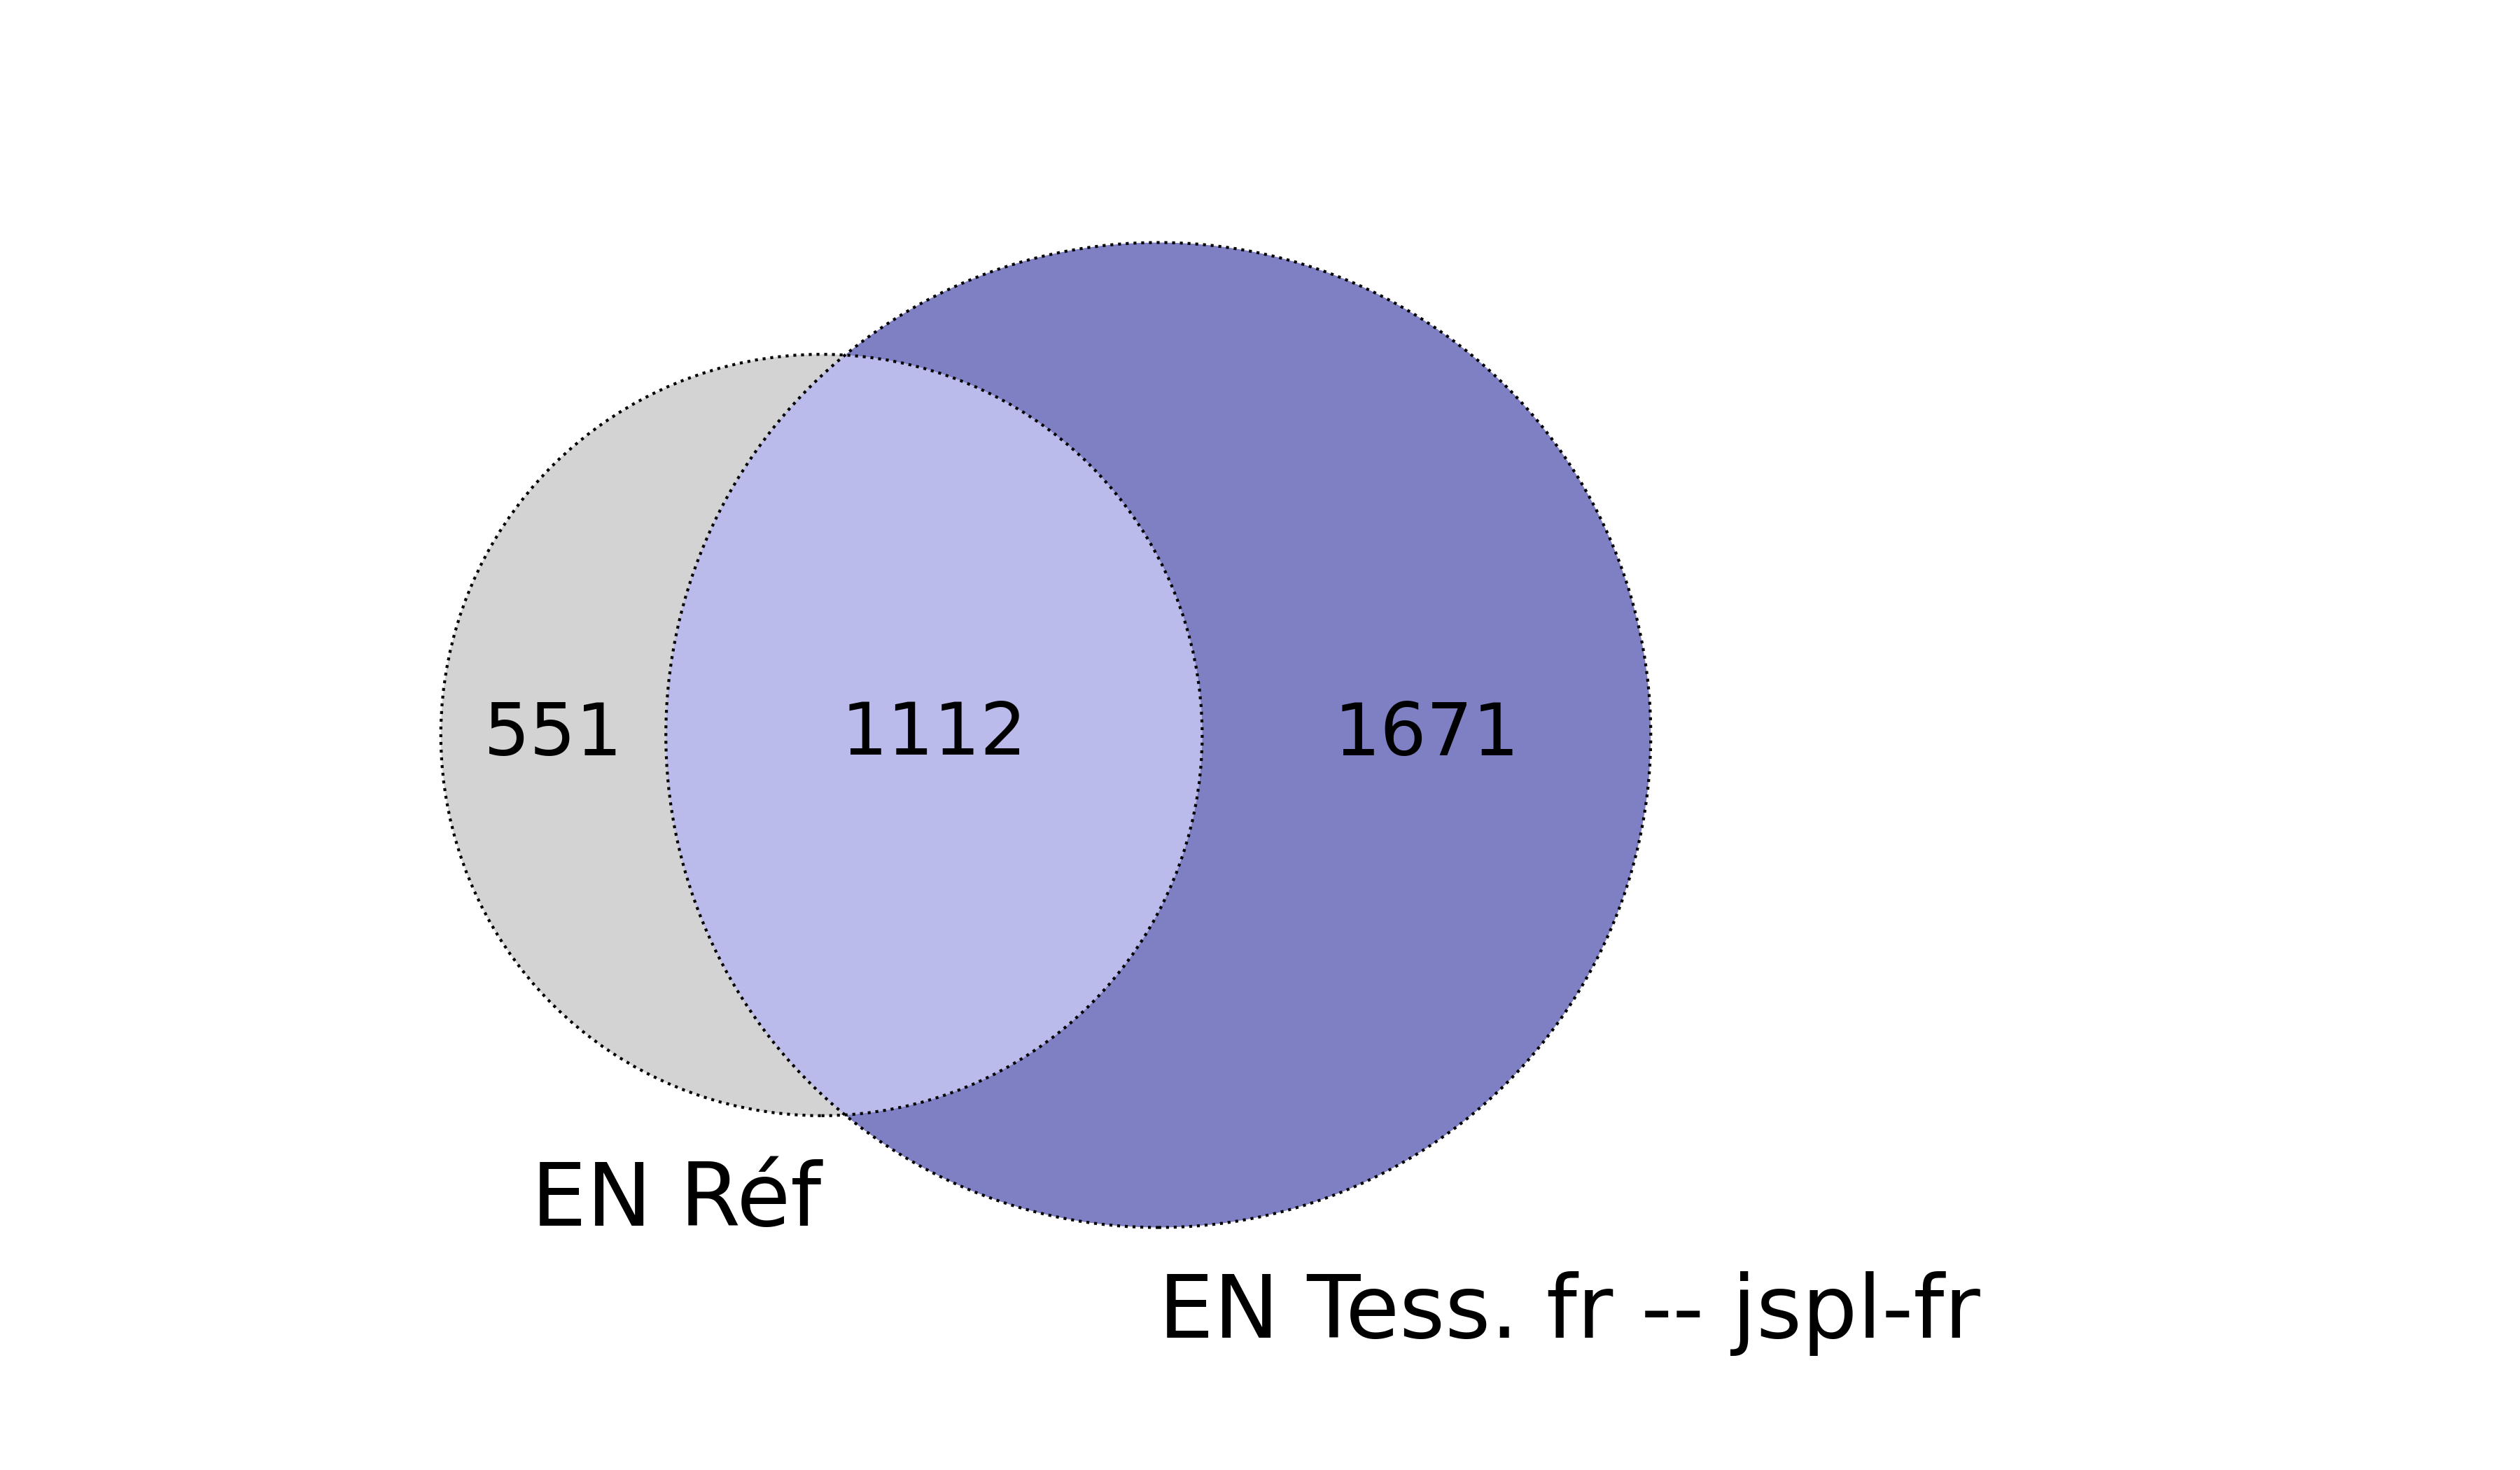
\includegraphics[width=1\textwidth]{IMAGES/INTERSECTIONS_GLOBALES/ELTeCFRA_Tess. fr -- jspl-fr_stanza-concat_intersection.png}
  \caption{Tess. fr. corrigé -- \texttt{stanza}}
  \label{fig:ELTeCFRA_Tess. fr -- jspl-fr_stanza-concat_intersection}
  \end{subfigure}
    \end{minipage}
\caption{Intersections pour la configuration Tess-\texttt{spaCy\_lg} corrigées avec le modèle pré-entrainer de JamSpell et le modèle ELTeC, pour le sous-corpus ELTeC français.}
\label{fig:intersection-globale-tess}
\end{figure}

\subsubsection{Mesures de distance textuelle}
\label{sec:distances_creux}
Dans le but de mener une évaluation plus souple des résultats de REN sur les sorties de ROC bruitées et leurs corrections automatiques, nous avons employé des mesures de distance. Nous avons privilégié les métriques de Jaccard et cosinus car elles sont considérées comme des mesures de référence quand il est question de (dis)similarité textuelle \cite{buscaldi2020calcul}. La figure \ref{fig:distance_texte} illustre les résultats obtenus pour les textes de référence et les différentes versions de ROC pour le sous-corpus ELTeC portugais avec les mesures de jaccard et cosinus, et les résultats pour les autres sous-corpus de notre études sont similaires. Les figures \ref{fig:spaCy3.5.1-lg} et \ref{fig:Cosinus-spacy-lg-stanza} montrent les résultats obtenus en comparant les sorties de REN obtenues sur les textes de référence et celles des différentes configurations évaluées (tableau \ref{tab:config}). Pour lire ces figures, il faut noter que plus la boîte est proche de zéro, plus les sorties comparées sont similaires.
Après une observation des différentes mesures de distance présentées pour chaque sous-corpus évalué, on note l'écart constant et considérable entre les résultats de Jaccard et cosinus. Les résutats pour Jaccard sont souvent proches de 1, tandis que ceux de cosinus sont proches de 0 pour les comparaisons des mêmes configurations. Il semble que la métrique cosinus sous-estime la distance entre les résultats pour les configurations de ROC et celles de référence. 

\begin{figure}
   \centering
      \begin{subfigure}{0.45\textwidth}
  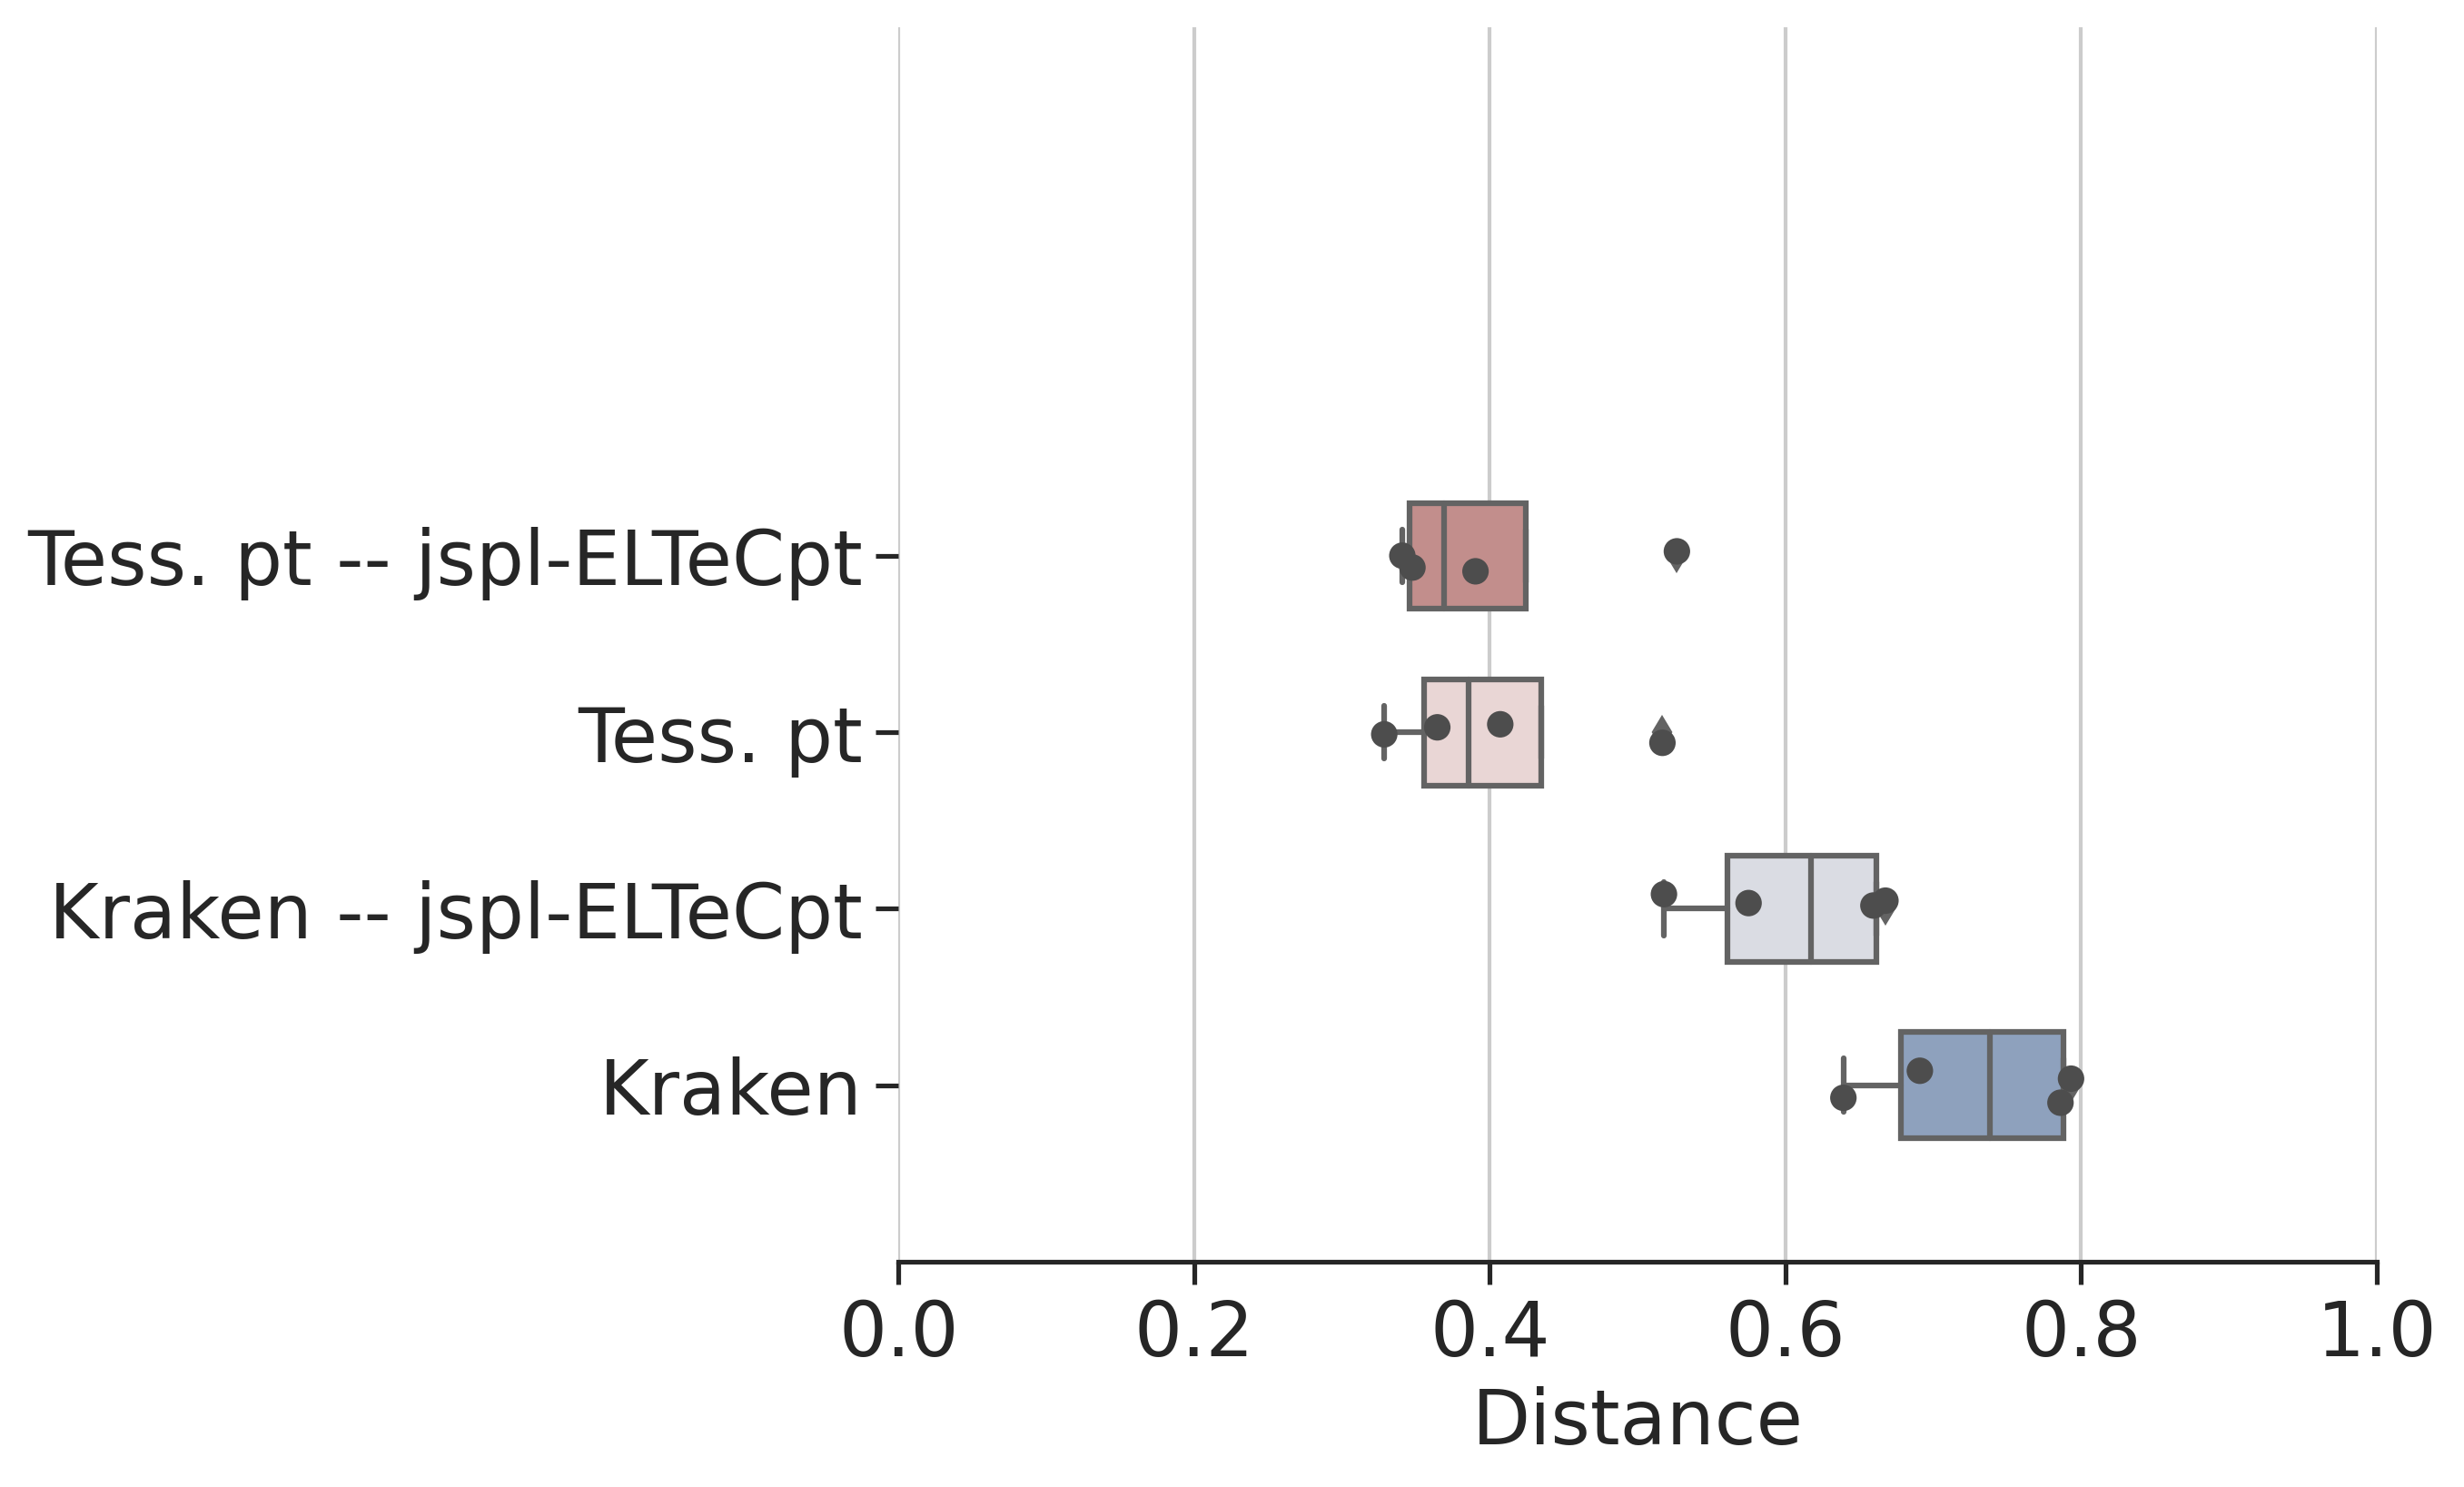
\includegraphics[height=.65\textwidth]{IMAGES/Boite-moustache/ELTeC-Por_REF_jaccard.png} 
        \caption{ELTeC-Por Jaccard}
   \end{subfigure}
    \begin{subfigure}{0.5\textwidth}
  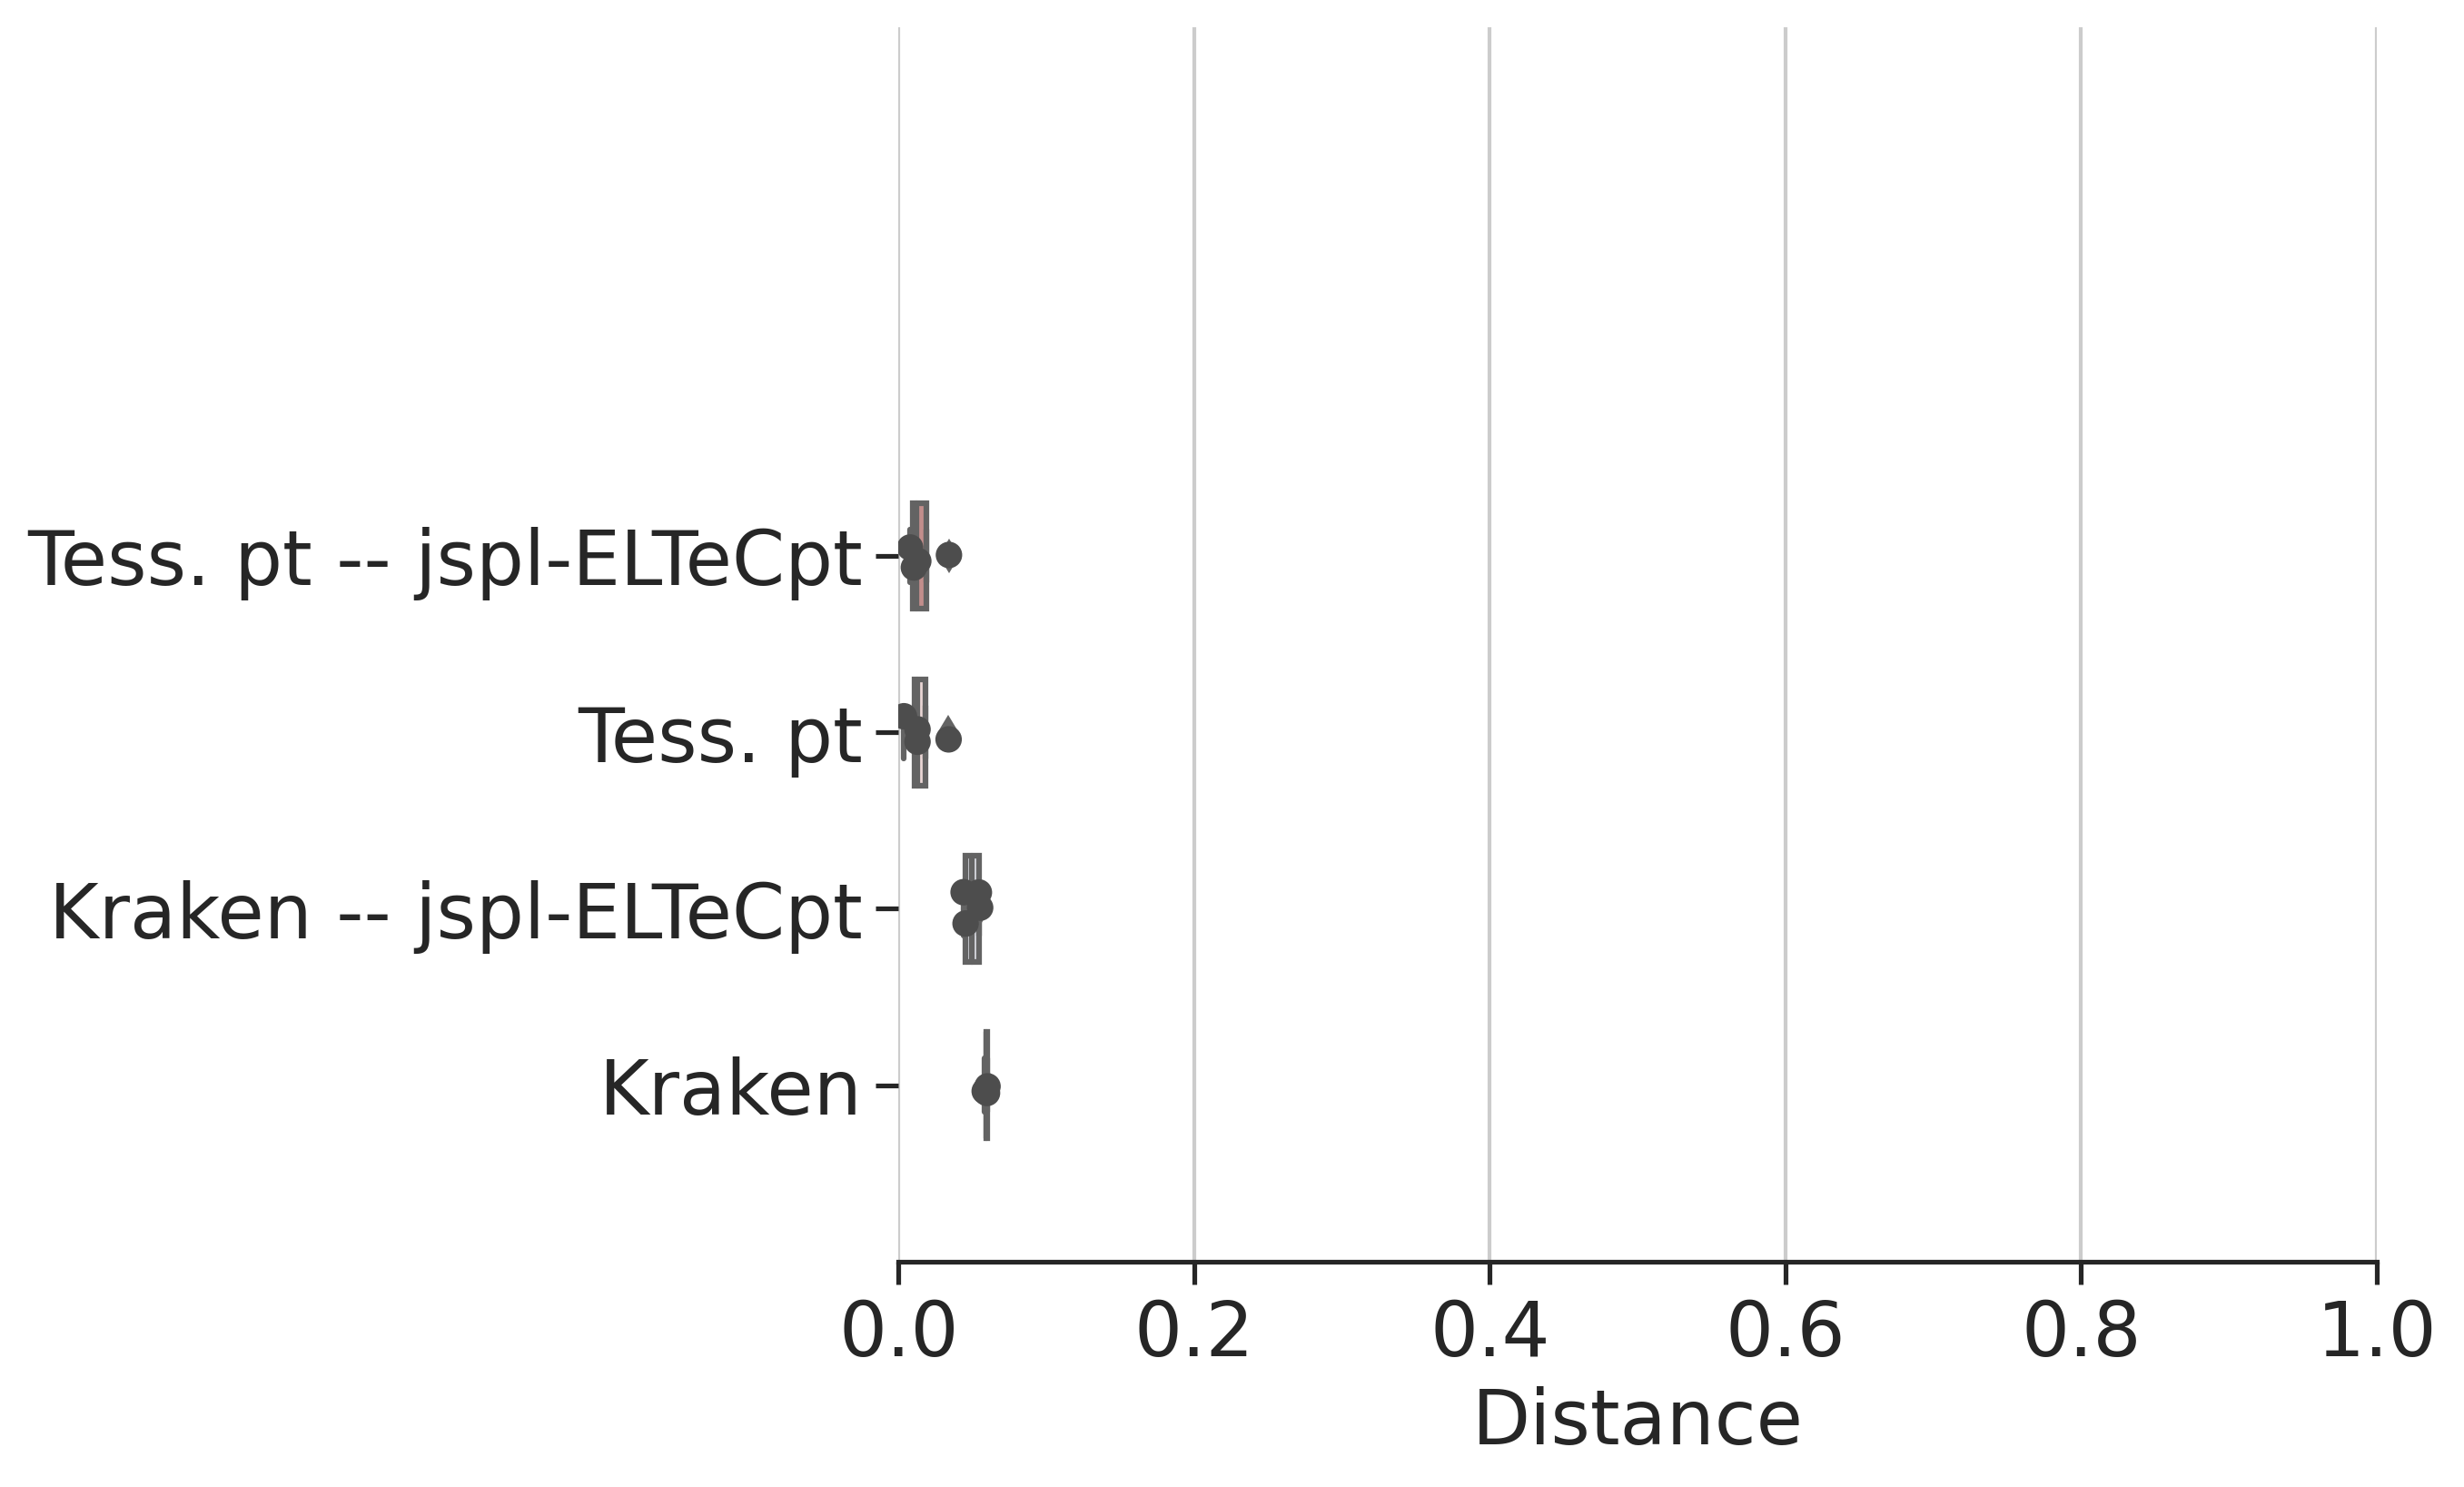
\includegraphics[height=.65\textwidth]{IMAGES/Boite-moustache/ELTeC-Por_REF_cosinus.png} 
        \caption{ELTeC-Por cosinus}
   \end{subfigure}   
    \caption{Distances calculées entre les textes de référence et les versions de ROC.}
    \label{fig:distance_texte}
\end{figure}

%% TODO GL: Alignement des figures boites à moustache
\begin{figure}
   \centering
         \begin{subfigure}{0.45\textwidth}
  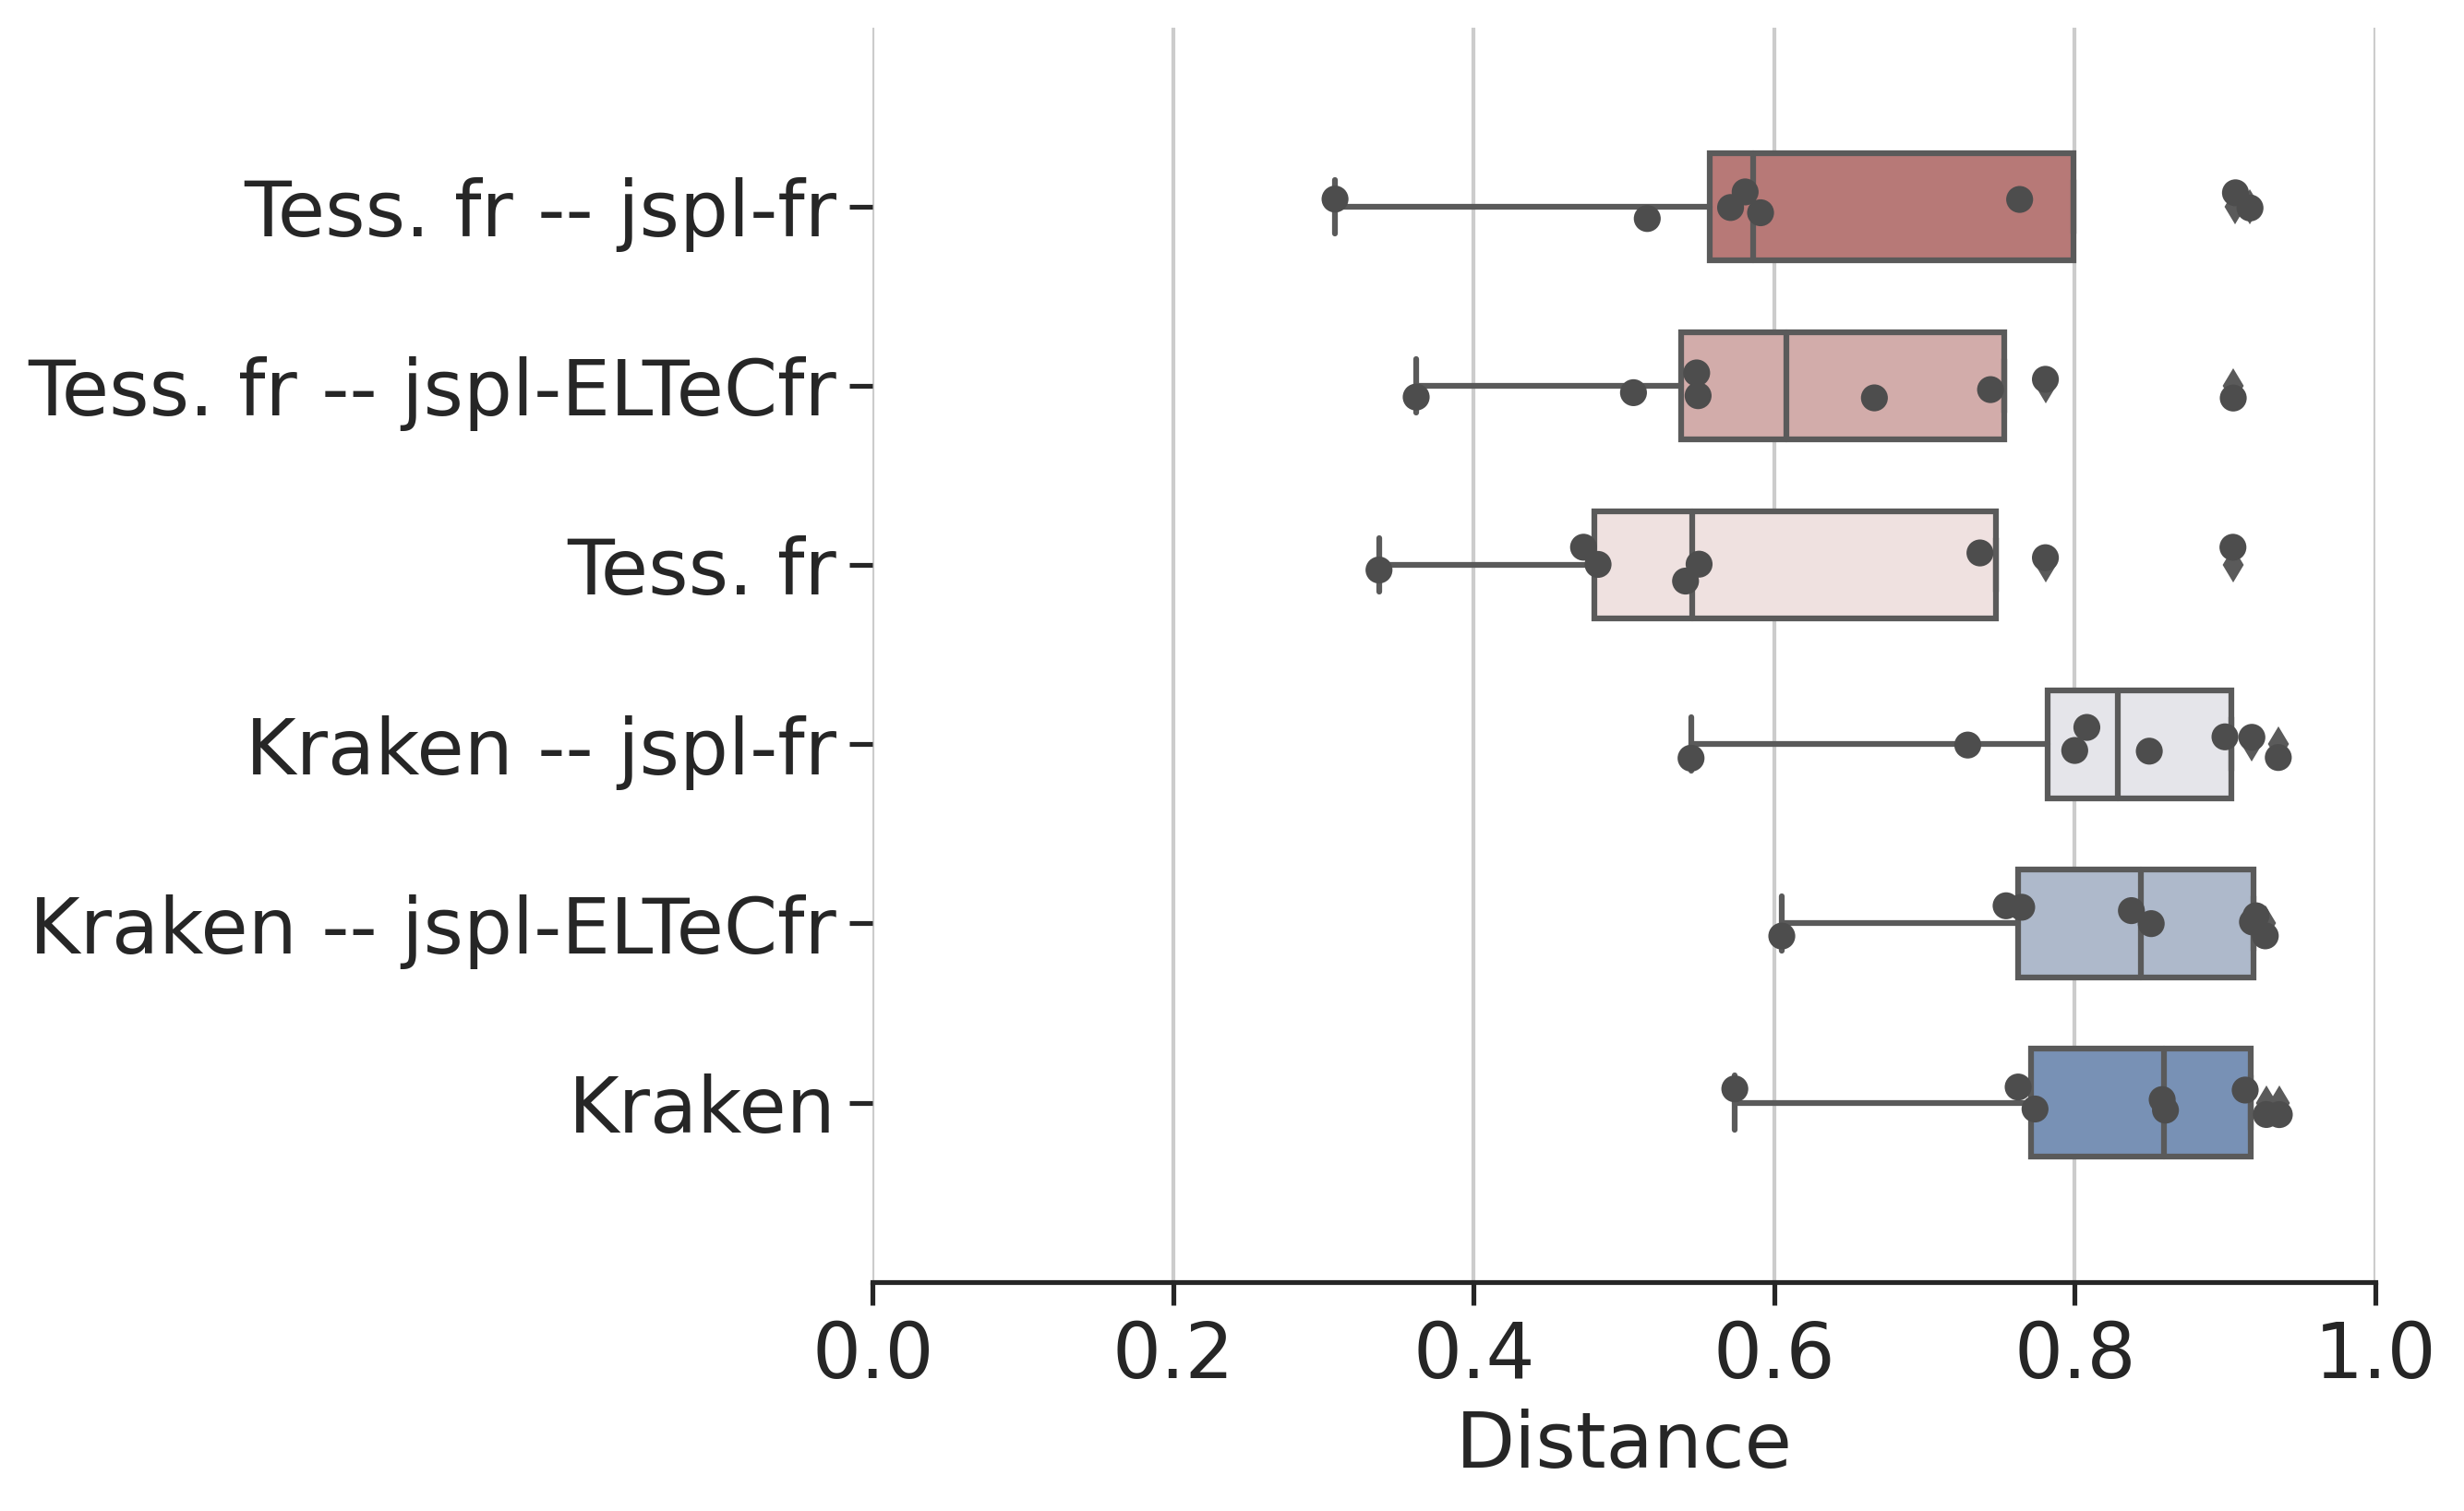
\includegraphics[height=.65\textwidth]{IMAGES/Boite-moustache/TGB_spaCy3.5.1_jaccard.png} 
        \caption{TGB Jaccard}
   \end{subfigure}
    \begin{subfigure}{0.5\textwidth}
  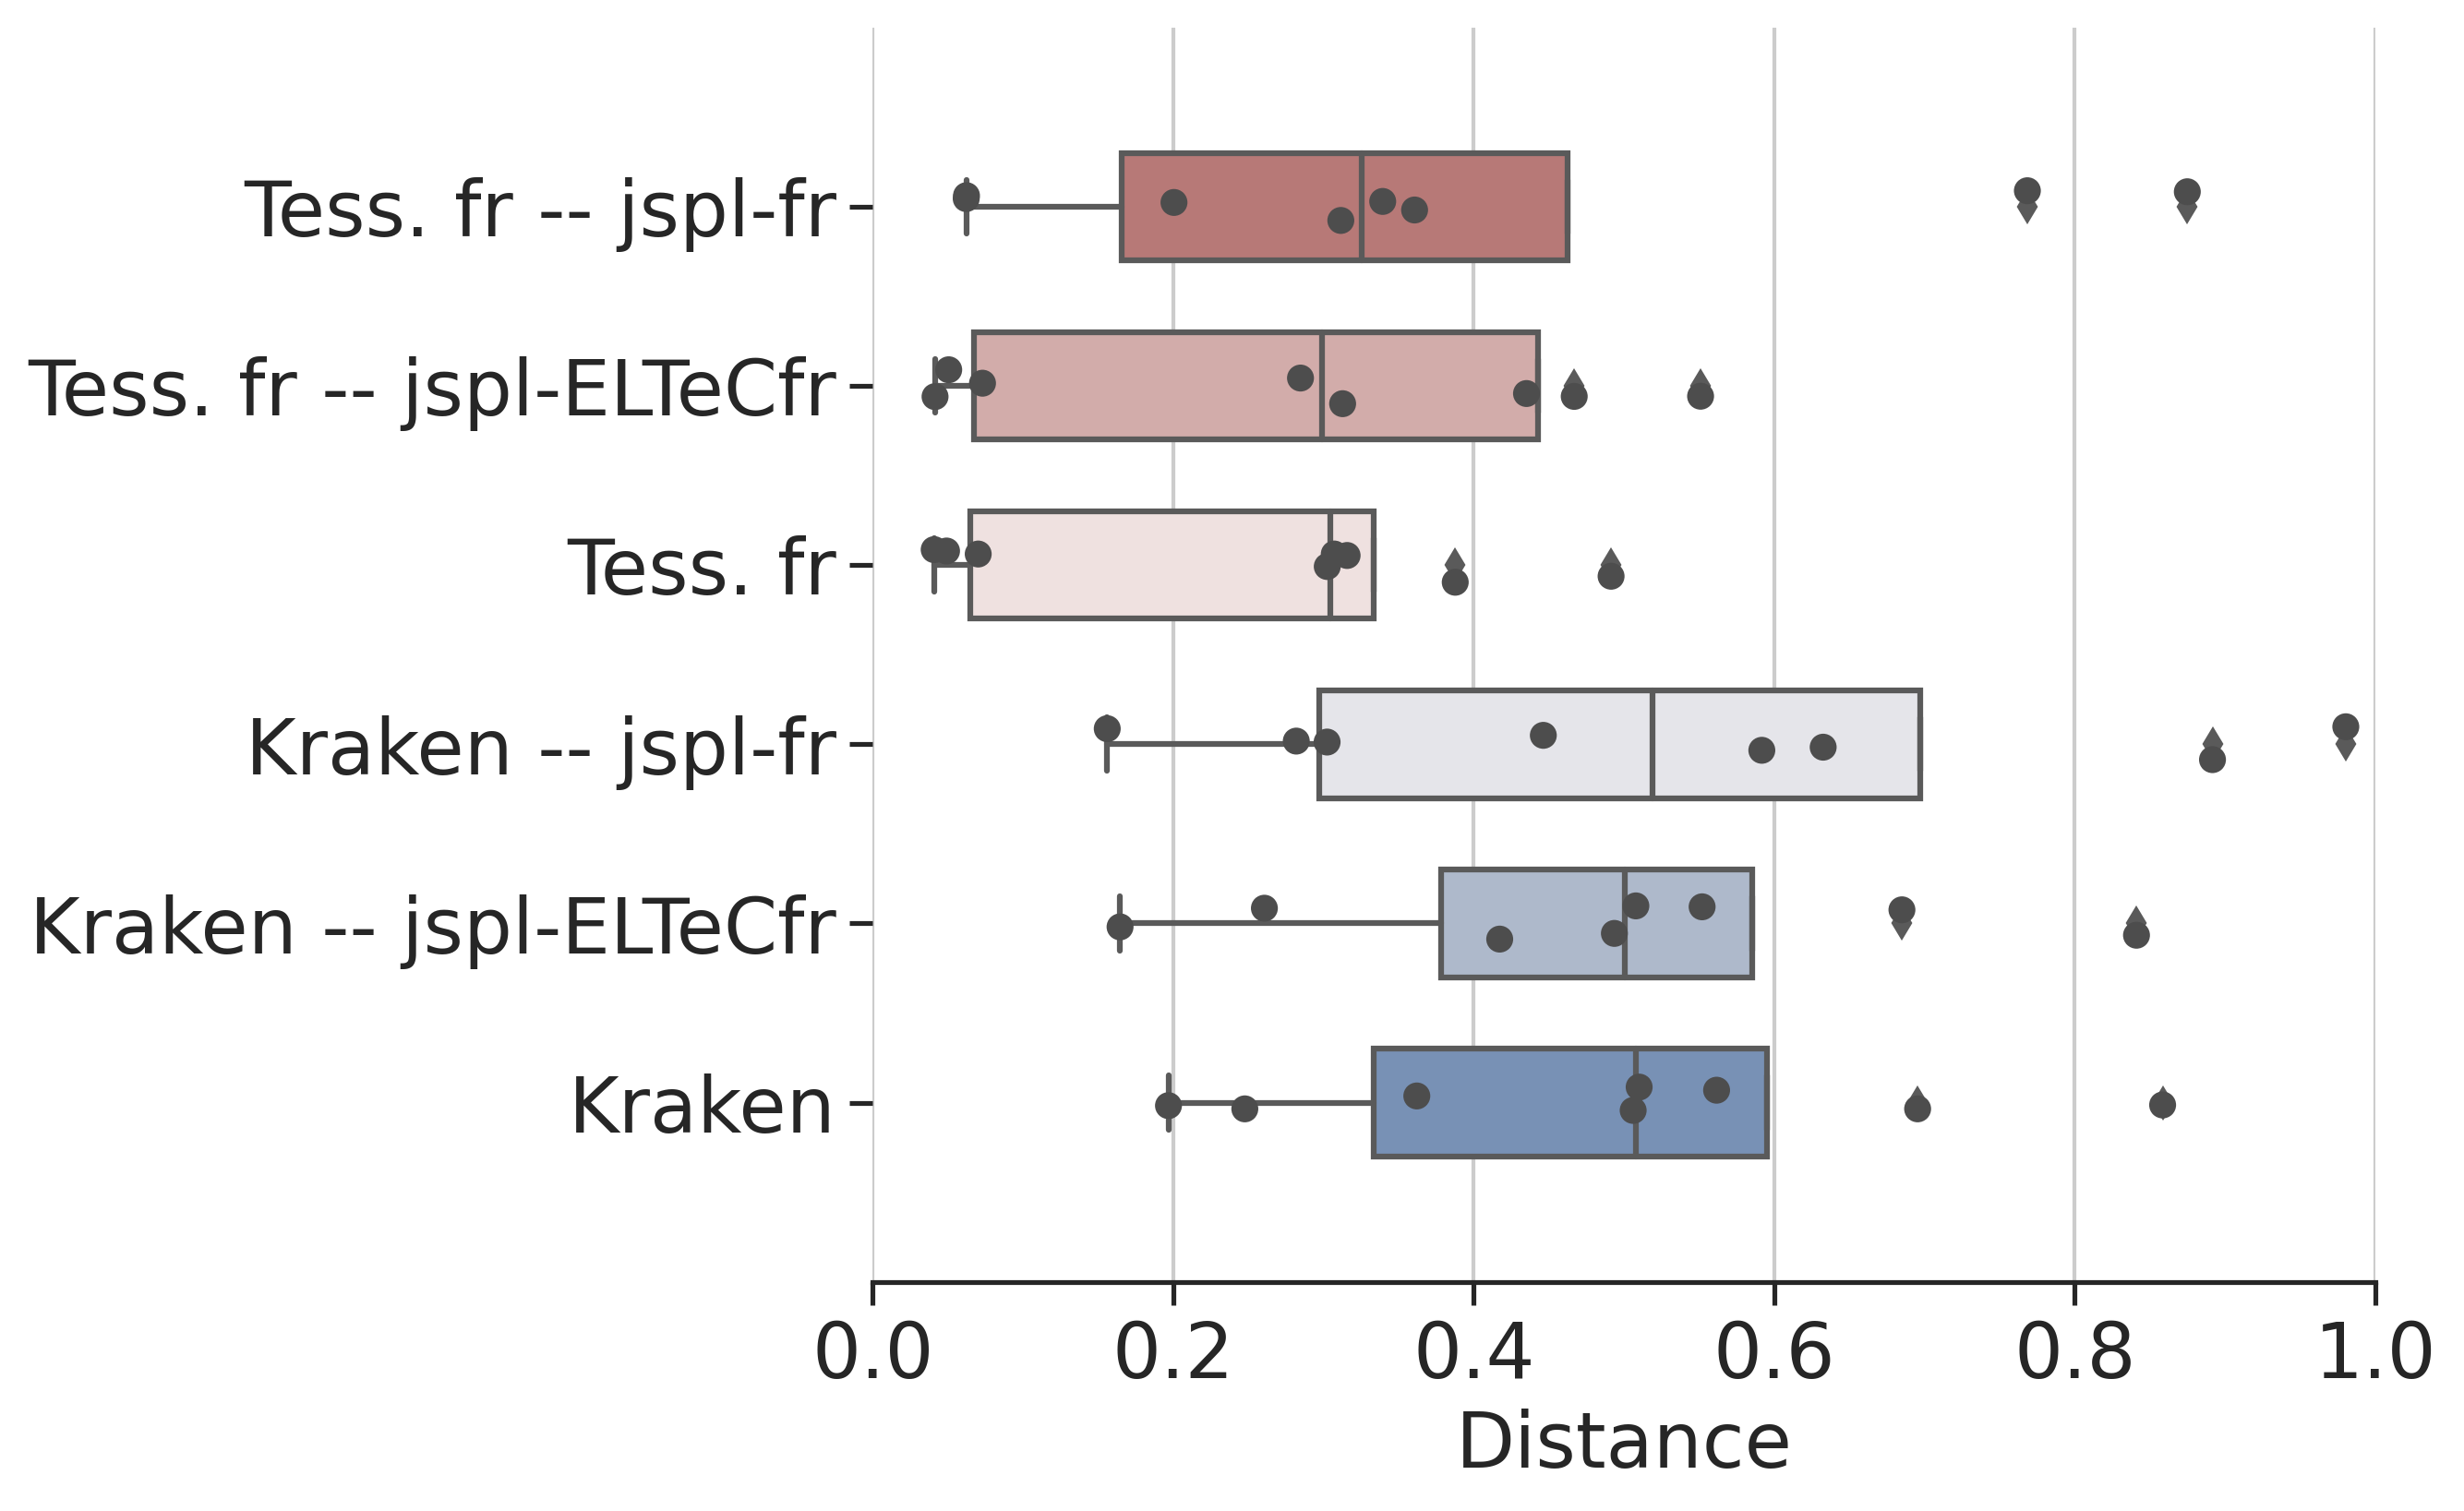
\includegraphics[height=.65\textwidth]{IMAGES/Boite-moustache/TGB_spaCy3.5.1_cosinus.png} 
        \caption{TGB cosinus}
   \end{subfigure}
   
    \caption{\texttt{spaCy\_lg}.}
    \label{fig:spaCy3.5.1-lg}
\end{figure}

Pour préciser notre réflexion s'appuyant sur la lecture des figures \ref{fig:distance_texte}, \ref{fig:spaCy3.5.1-lg} et \ref{fig:Cosinus-spacy-lg-stanza} nous avons procédé à la lecture des figures analogues obtenues pour chacun des autres sous-corpus et consulté manuellement les résultats effectifs de REN. Finalement, cette différence entre les résultats de Jaccard et cosinus pourrait s'expliquer par le fait que la première mesure prend en compte le vocabulaire, alors que la seconde s'intéresse aux nombre d'occurrences d'une EN. Concrètement, cela signifie pour la distance de Jaccard que si le vocabulaire entre les sorties de deux ensemble pour les configurations comparées est très différent, le résultat est proche de 1. 
En revanche, les résultats pour la mesure cosinus dépendraient du nombre d'occurences de chaque EN dans les groupes comparés. Autrement dit, s'il y a beaucoup d'occurrences d'une EN dans une des configurations comparée mais qu'elle n'apparaît pas en même quantité dans les résultats de la seconde configuration, les résultats pour cosinus grimpent en flèche. L'observation des résultats roman par roman pour la mesure cosinus nous permet d'étayer cette hypothèse, en effet on dénombre, p.\ ex.\, 290 occurrences du terme ``INGLEZA'' pour la configuration Tesseract-pt--\texttt{spaCy\_lg}, alors qu'il apparaît 3 fois seulement dans les résultats de la configuration de référence\footnote{\textit{Uma familia ingleza}, Diniz.} -- dans ce dernier cas la valeur de cosinus est très élevée et dépasse celle de Jaccard (cos. : 0.69, Jaccard : 0.67). Il s'agit d'un comportement que nous avons pu observer régulièrement dans les résultats pour chacun des sous-corpus analysés.

La figure \ref{fig:Cosinus-spacy-lg-stanza} laisse apercevoir que les résultats pour la REN sur les versions Kraken des textes sont moins bons de manière générale que pour les versions produites avec Tesseract. Toutefois, il semblerait que la correction automatique soit un peu plus efficace sur les versions de Kraken avec le modèle JamSpell-ELTeC que sur les versions Tesseract, car l'écart entre les boîtes est plus grand. Cependant, les résultats des distances obtenus pour ces versions corrigées de Kraken restent inférieurs à ceux observés pour les versions Tesseract avec et sans corrections. Ces différents constats laissent à penser que plus une version de ROC est bruitée, plus le correcteur automatique intervient et produit de bonnes corrections (figure \ref{fig:Cosinus-spacy-lg-stanza}f.). À l'inverse, si une version de ROC est peu bruitée, alors le correcteur automatique aura tendance à moins bien corriger, voire à sur-corriger. On peut observer ce phénomène concernant les résultats de la REN sur Tesseract qui sont moins bons sur les versions Tesseract corrigées. 

%\footnote{Nous analysons les résultats obtenus par ce moteur d'OCR puisqu'il présente moins de fluctuations des valeurs réparties sur les trois catégories de textes -- version non corrigée, version corrigée avec JamSpell pré-entraîné et celle corrigée avec JamSpell ELTeC.} 

%Nous avons identifié une tendance des métriques à illustrer un grand écart entre les valeurs des versions non corrigées et corrigées, notamment dans les figures a.\ et b. Ce \og{}phénomène de creux\fg{} se caractérise par (i) le fait que les mesure de distance de cosinus des versions non corrigées soient bien supérieures à celles de versions corrigées et (ii) que l'écart entre les mesures de distance de soit plus prononcé.

Enfin, il apparaît en comparant les figures \ref{fig:spaCy3.5.1-lg} et \ref{fig:Cosinus-spacy-lg-stanza} que la configuration Tesseract--\texttt{spaCy\_lg}, en utilisant pour chacun des outils le modèle de langue adapté à la langue du sous-corpus étudié, soit la plus convaincante en considération du temps de calcul et des résultats. Pour 5 604 472 tokens\footnote{soit le texte brut pour le sous-corpus français de la version de référence et les versions Kraken et Tess. fr.} \texttt{stanza} prend 10 heures à fournir des résultats, alors que \texttt{spaCy} met 1 heure (Mémoire: 16Gio, CPU: Core™i5-1135G7). La lecture des tableaux \ref{tab:EN_contamines_Variantes} et \ref{tab:FP_VP} reportant les analyses manuelles met en évidence des résultats équivalents. 

\begin{figure}

    \begin{subfigure}{0.45\textwidth}
  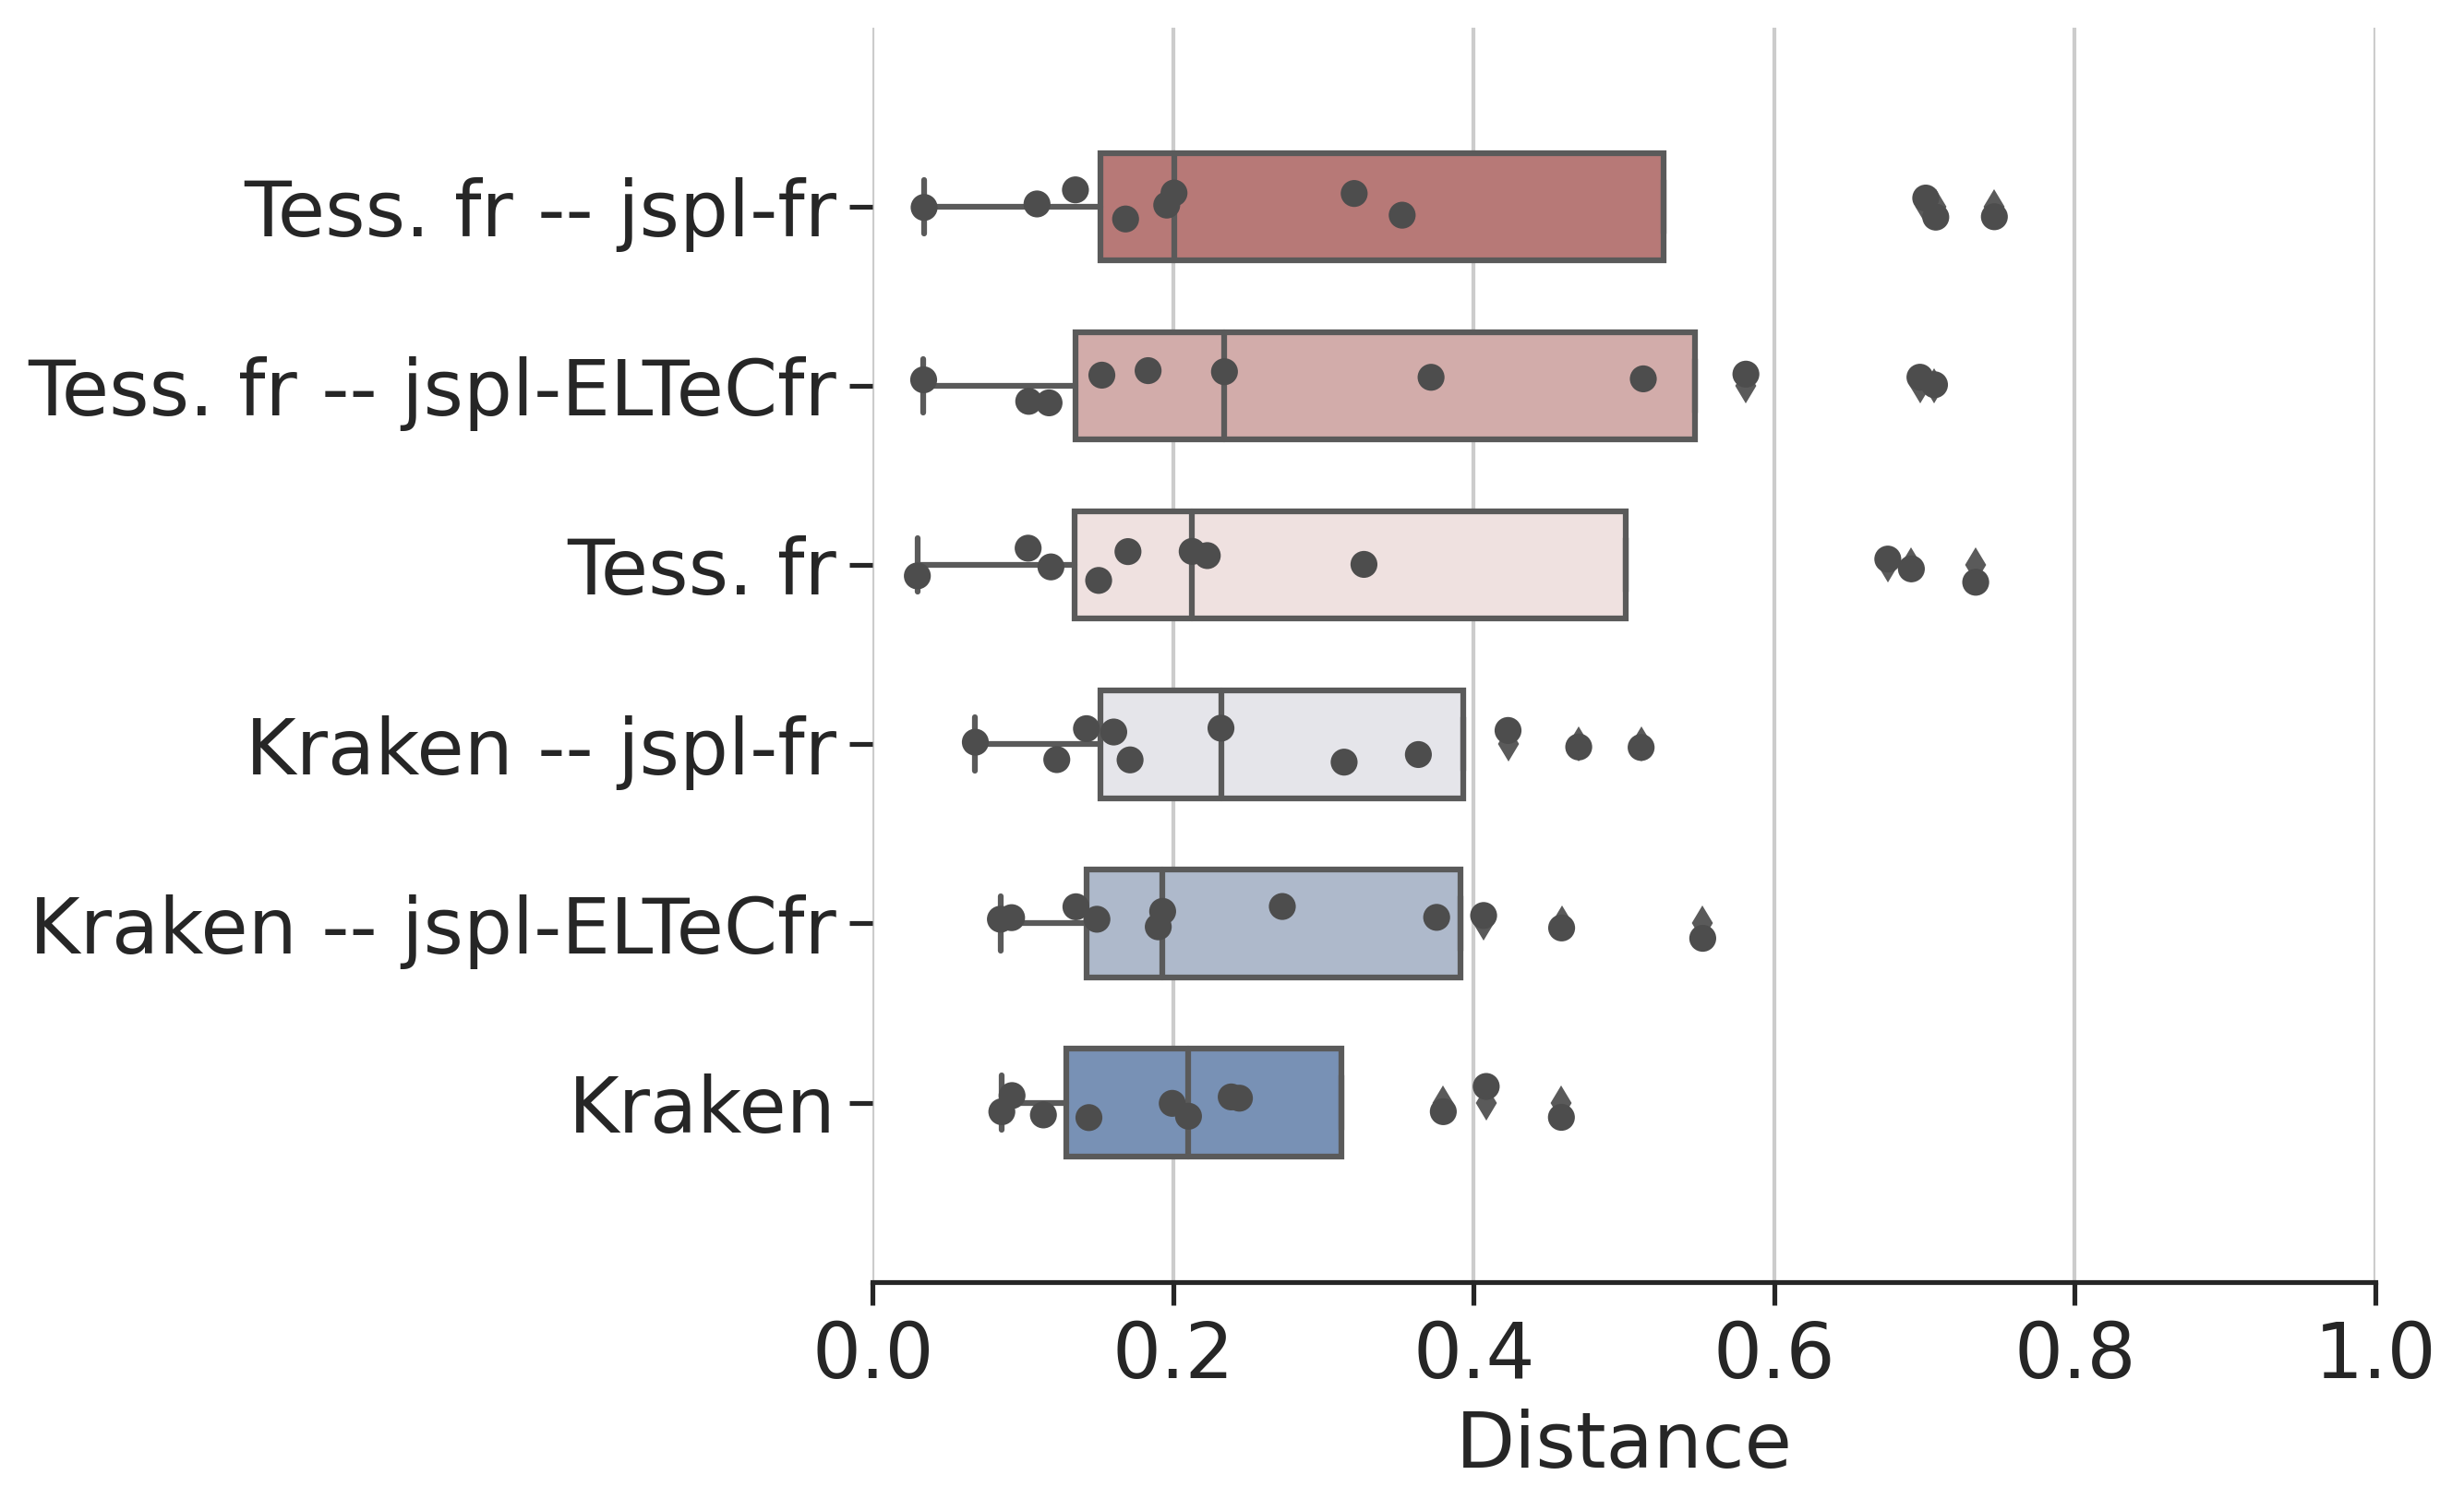
\includegraphics[height=.65\textwidth]{IMAGES/Boite-moustache/ELTeC-Fra_stanza_cosinus.png} 
        \caption{ELTeC-Fra \texttt{stanza} cosinus}
   \end{subfigure}
    \begin{subfigure}{0.5\textwidth}
  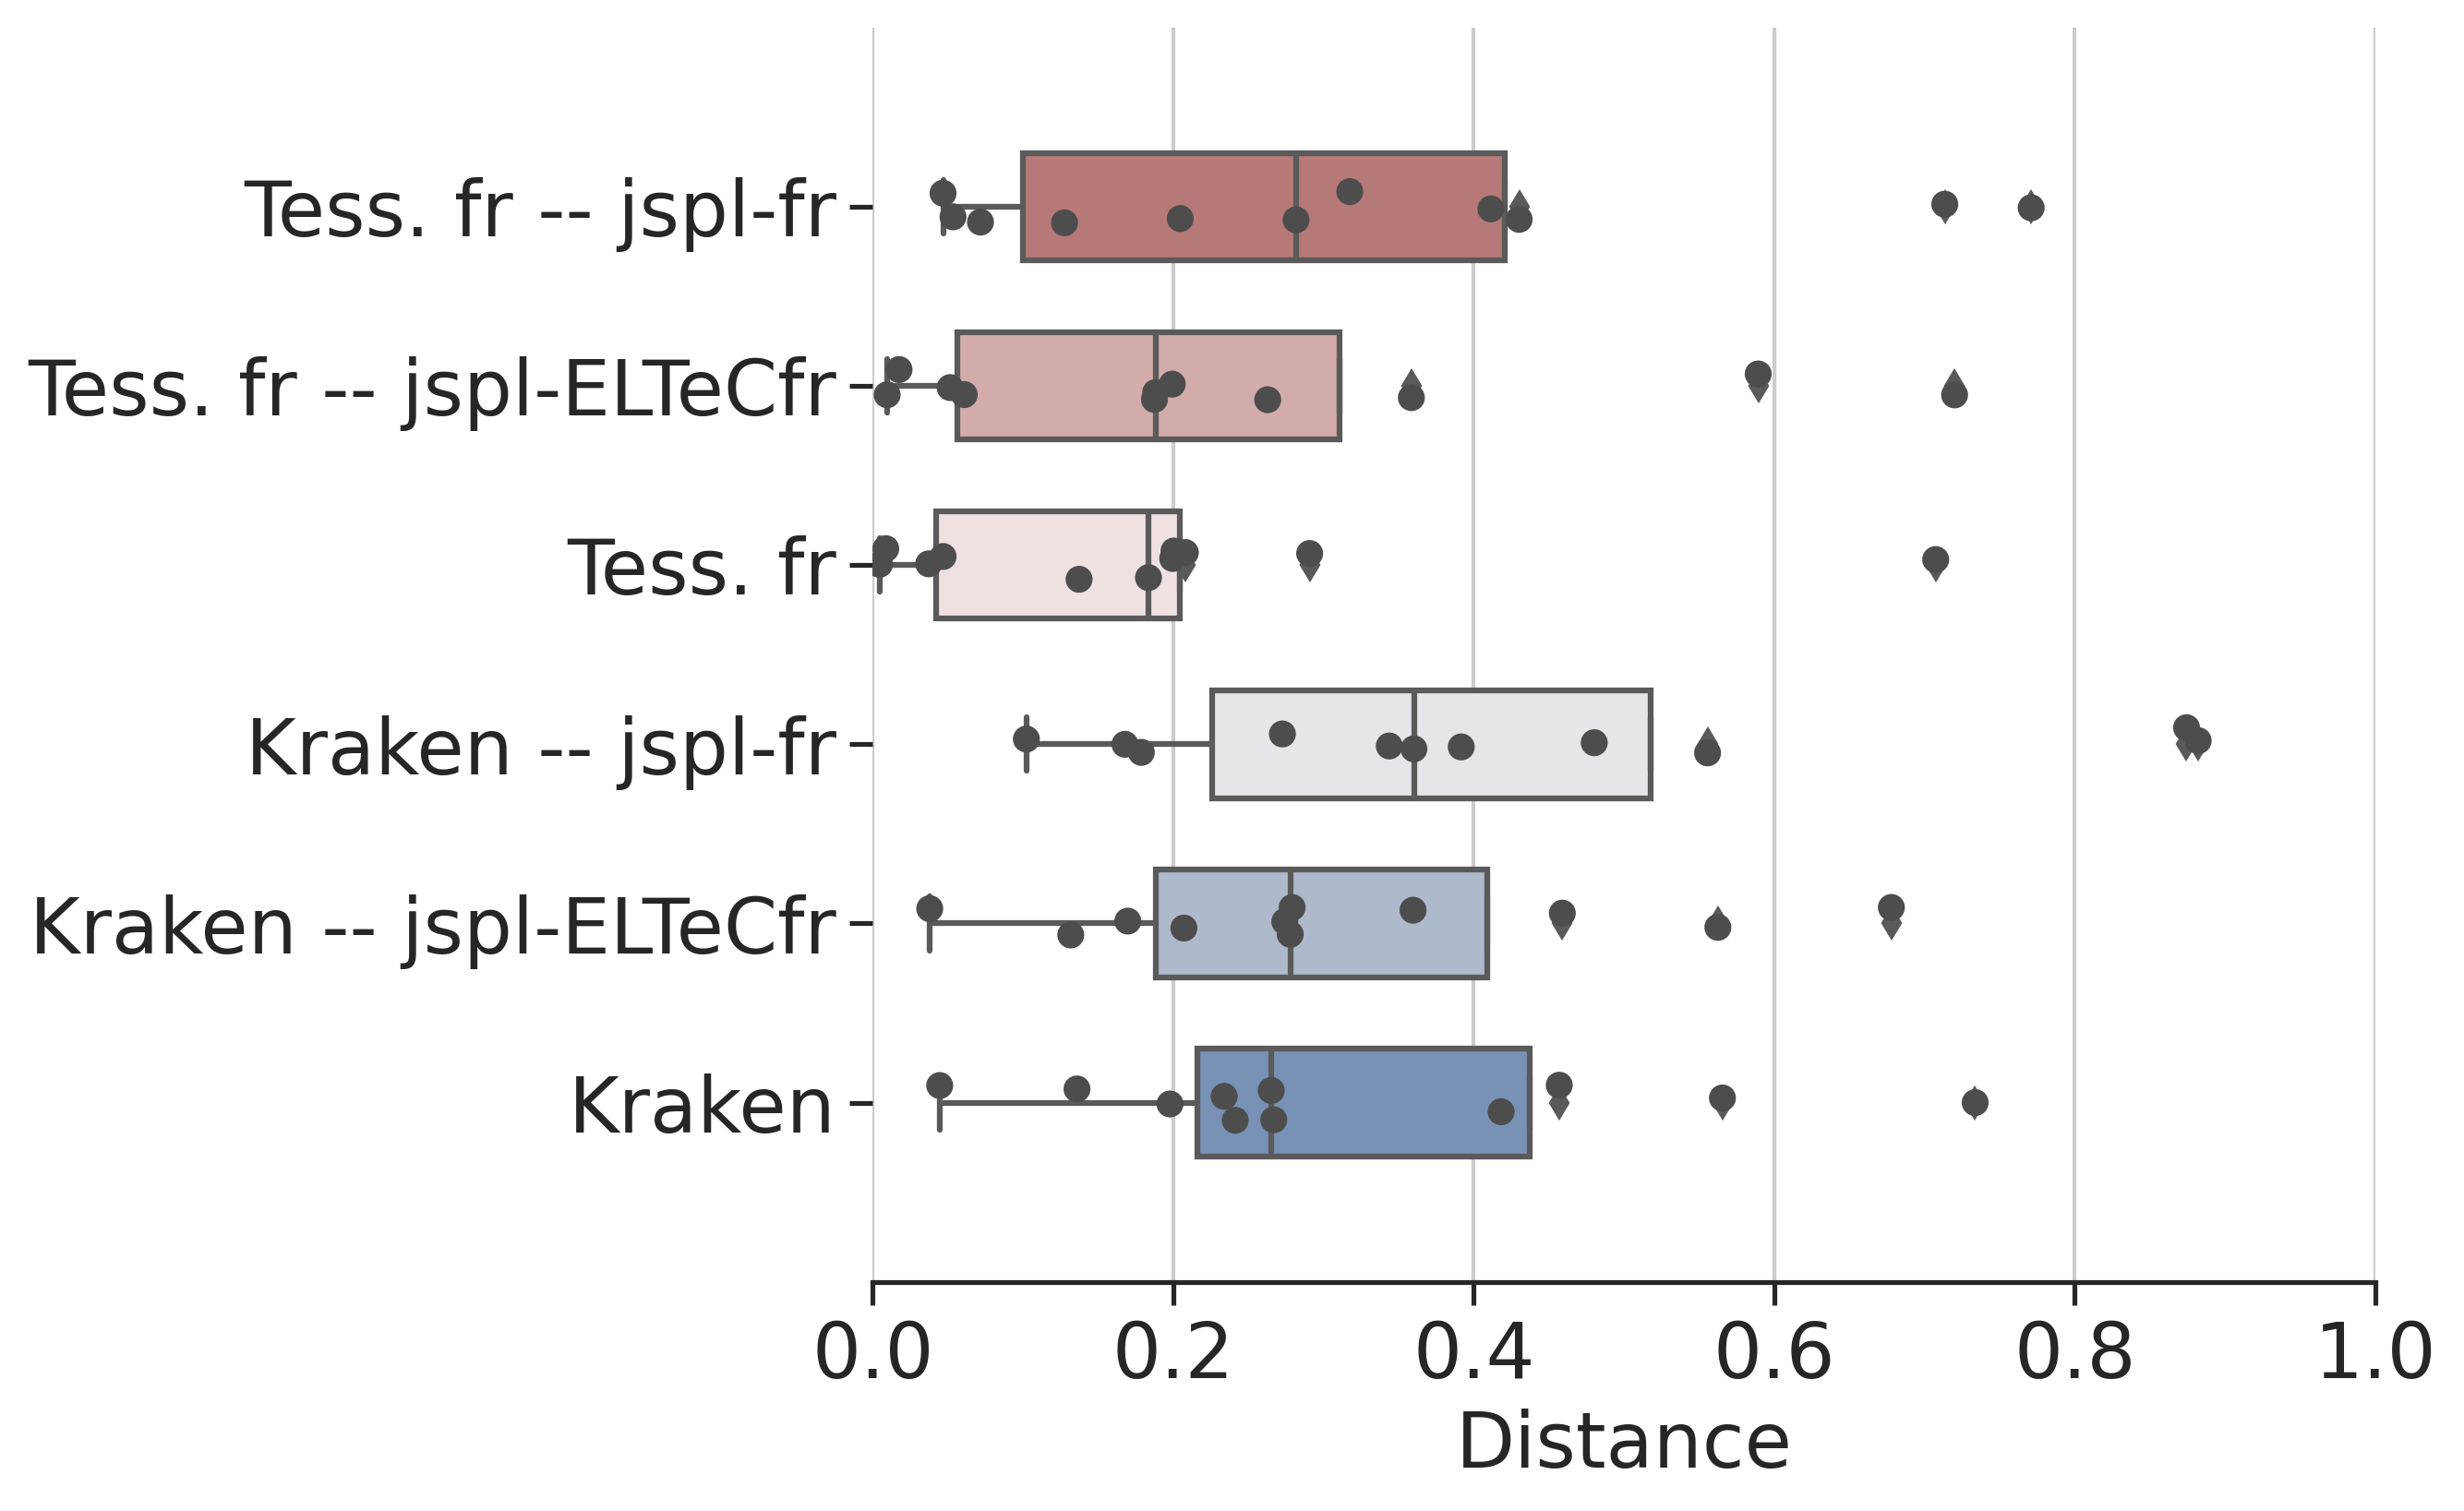
\includegraphics[height=.65\textwidth]{IMAGES/Boite-moustache/ELTeC-Fra_spacy3.5.1_cosinus.png} 
        \caption{ELTeC-Fra \texttt{spaCy} cosinus}
   \end{subfigure}

 \begin{subfigure}{0.45\textwidth}
  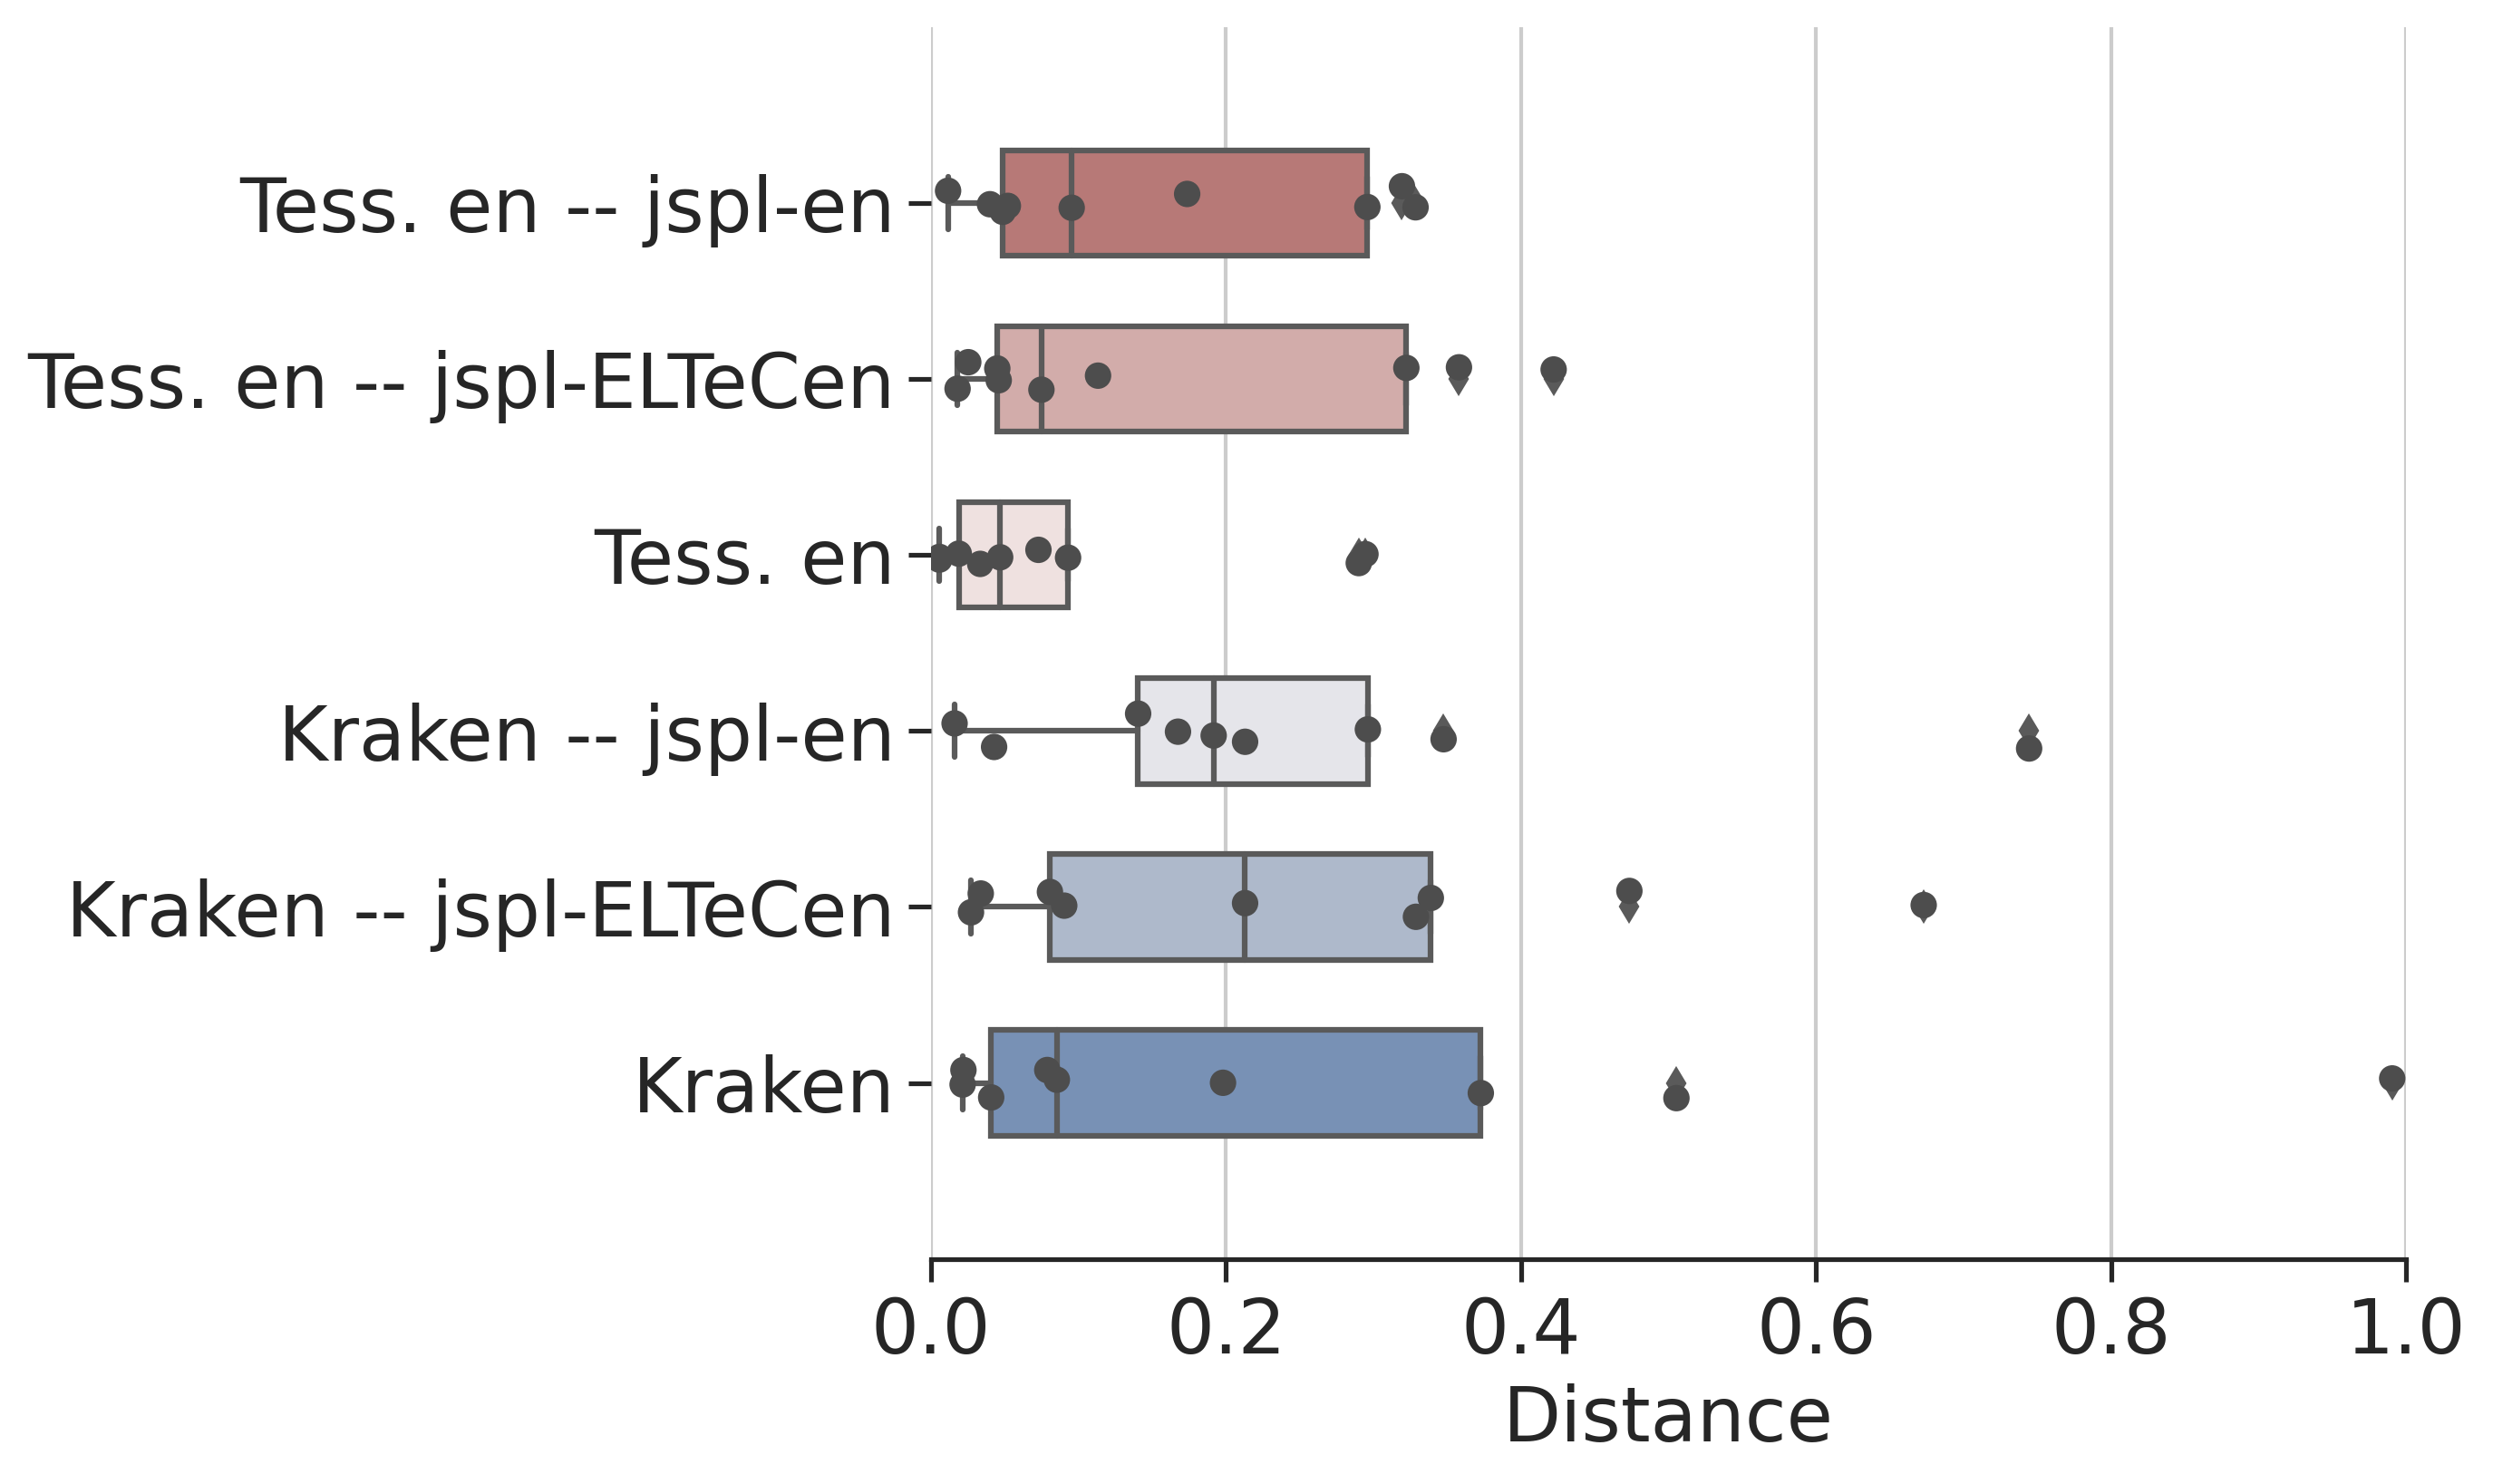
\includegraphics[height=.65\textwidth]{IMAGES/Boite-moustache/ELTeC-Eng_stanza_cosinus.png} 
        \caption{ELTeC-Eng \texttt{stanza} cosinus}
   \end{subfigure}
    \begin{subfigure}{0.5\textwidth}
  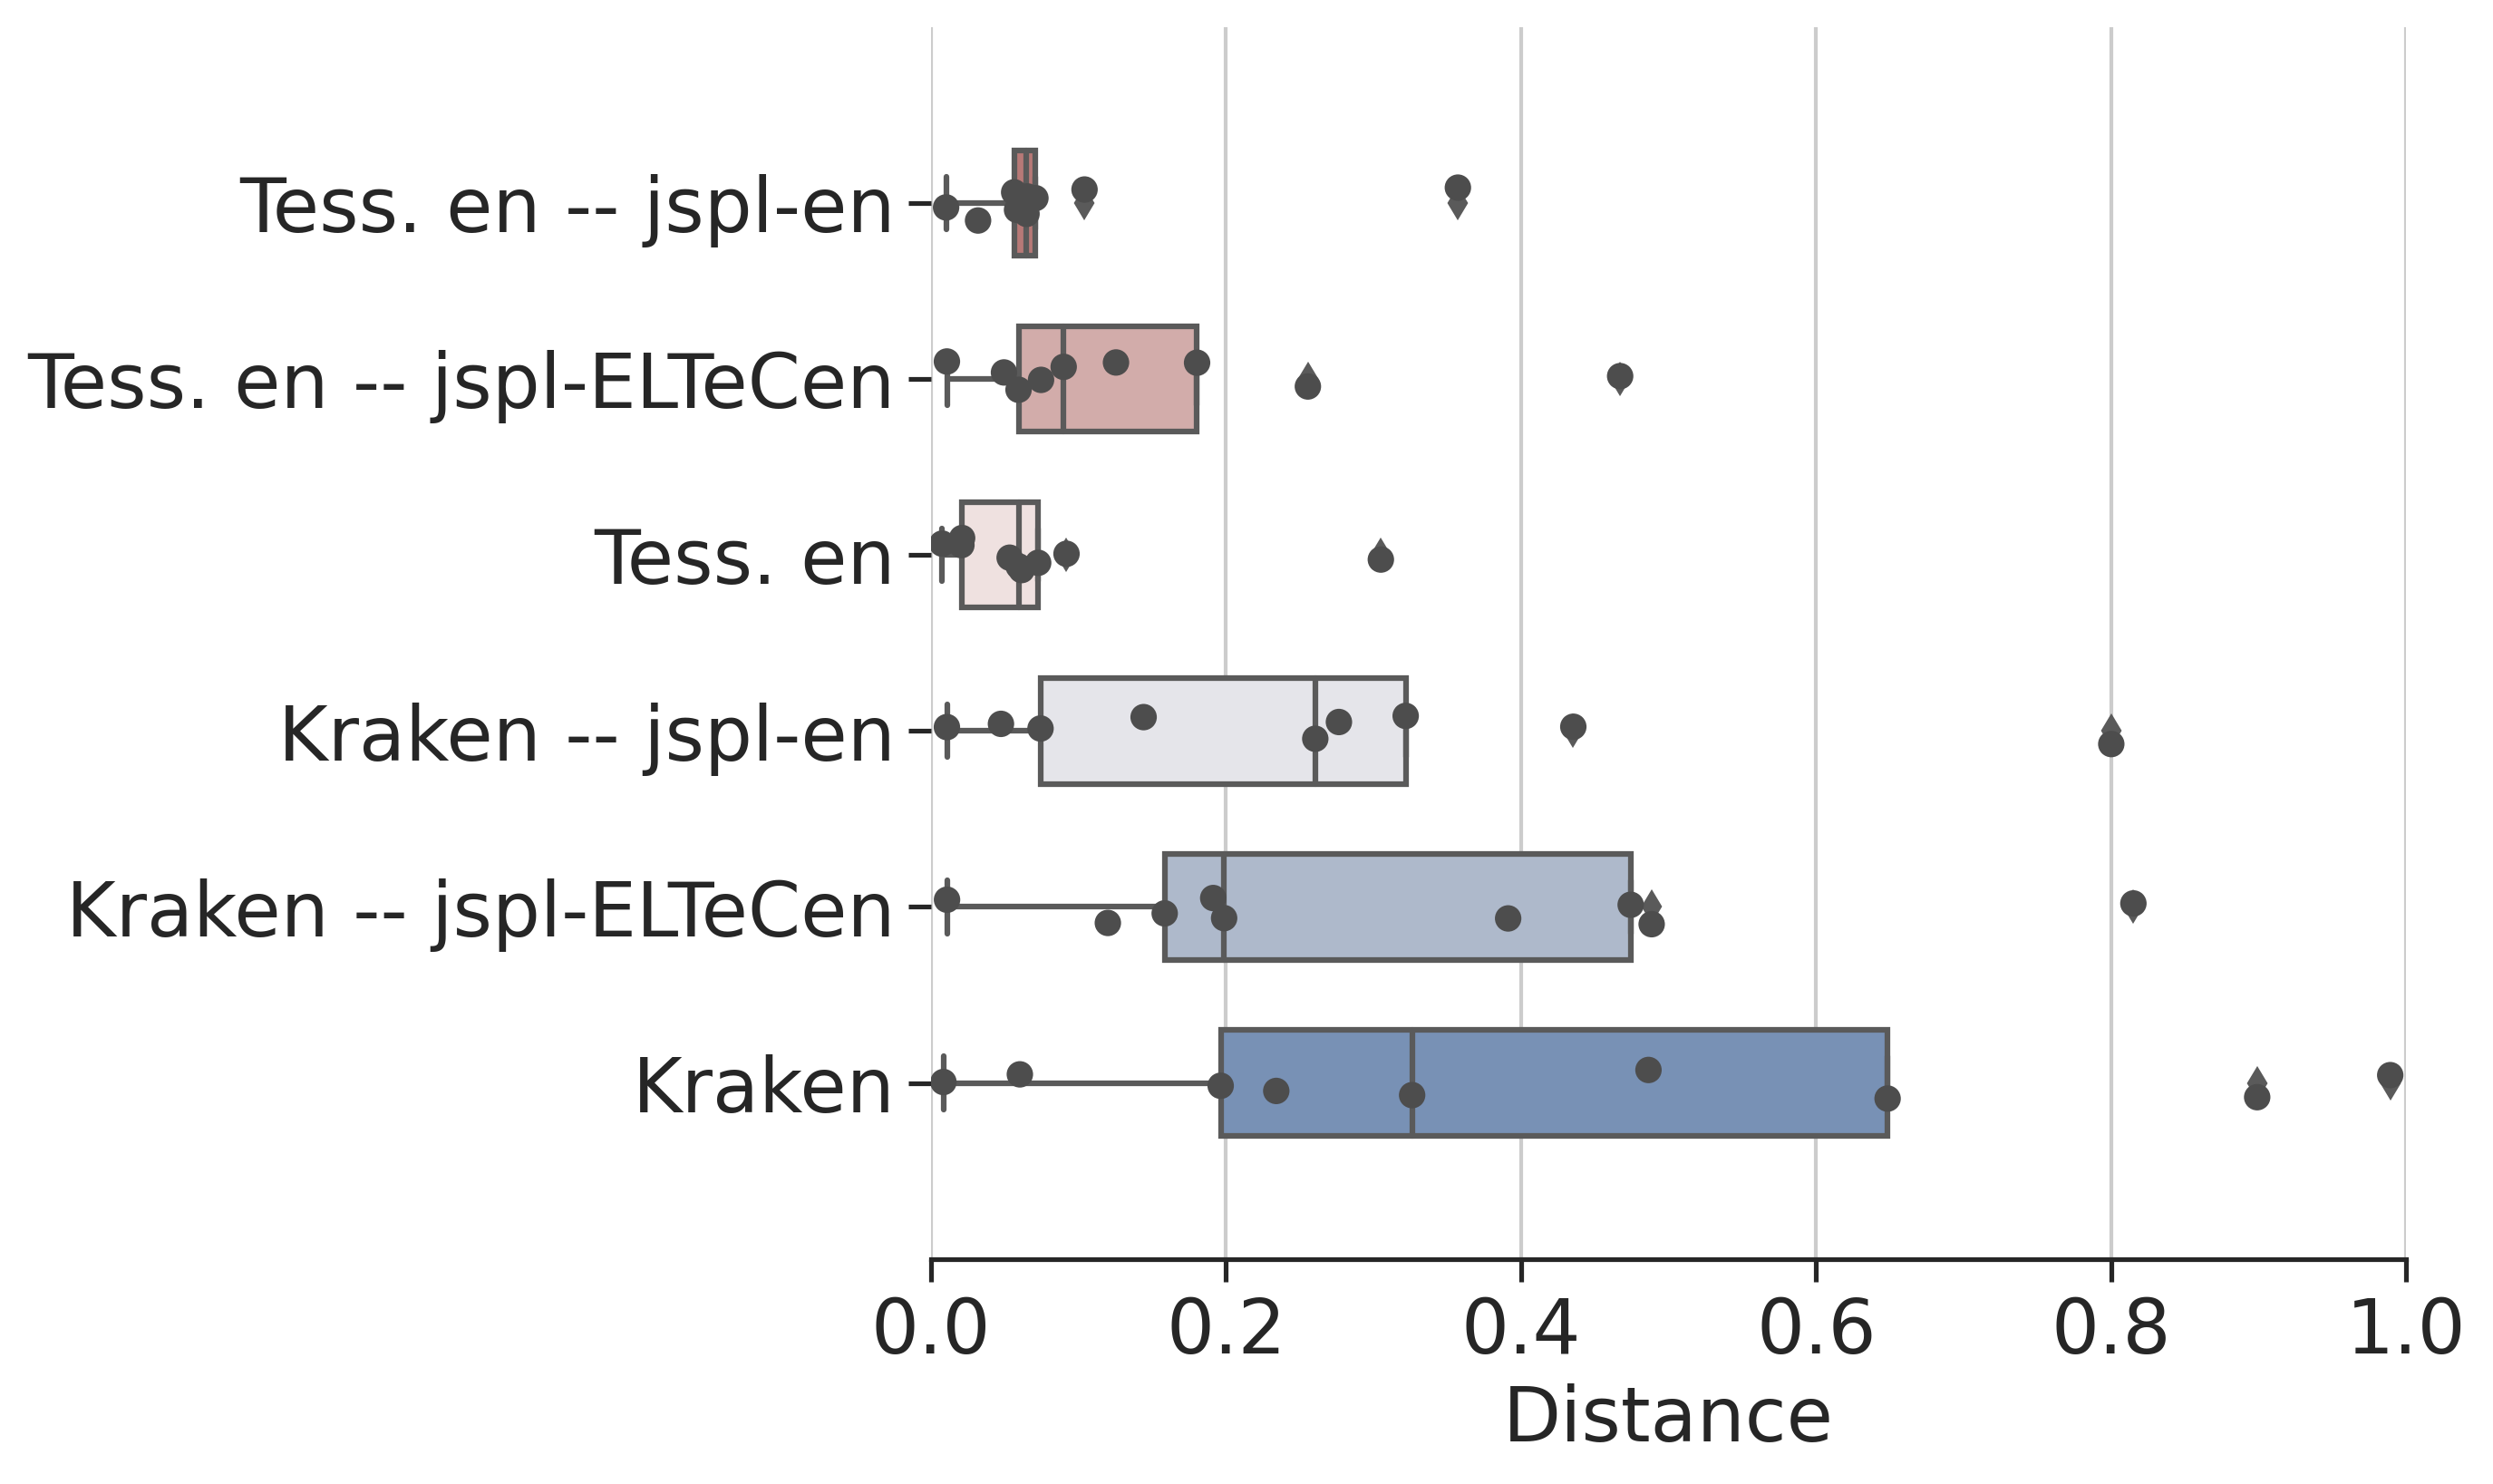
\includegraphics[height=.65\textwidth]{IMAGES/Boite-moustache/ELTeC-Eng_spacy3.5.1_cosinus.png} 
        \caption{ELTeC-Eng \texttt{spaCy} cosinus}
   \end{subfigure}

      \begin{subfigure}{0.45\textwidth}
  %\includegraphics[height=.65\textwidth]{} 
        \caption*{}
   \end{subfigure}
    \begin{subfigure}{0.5\textwidth}
  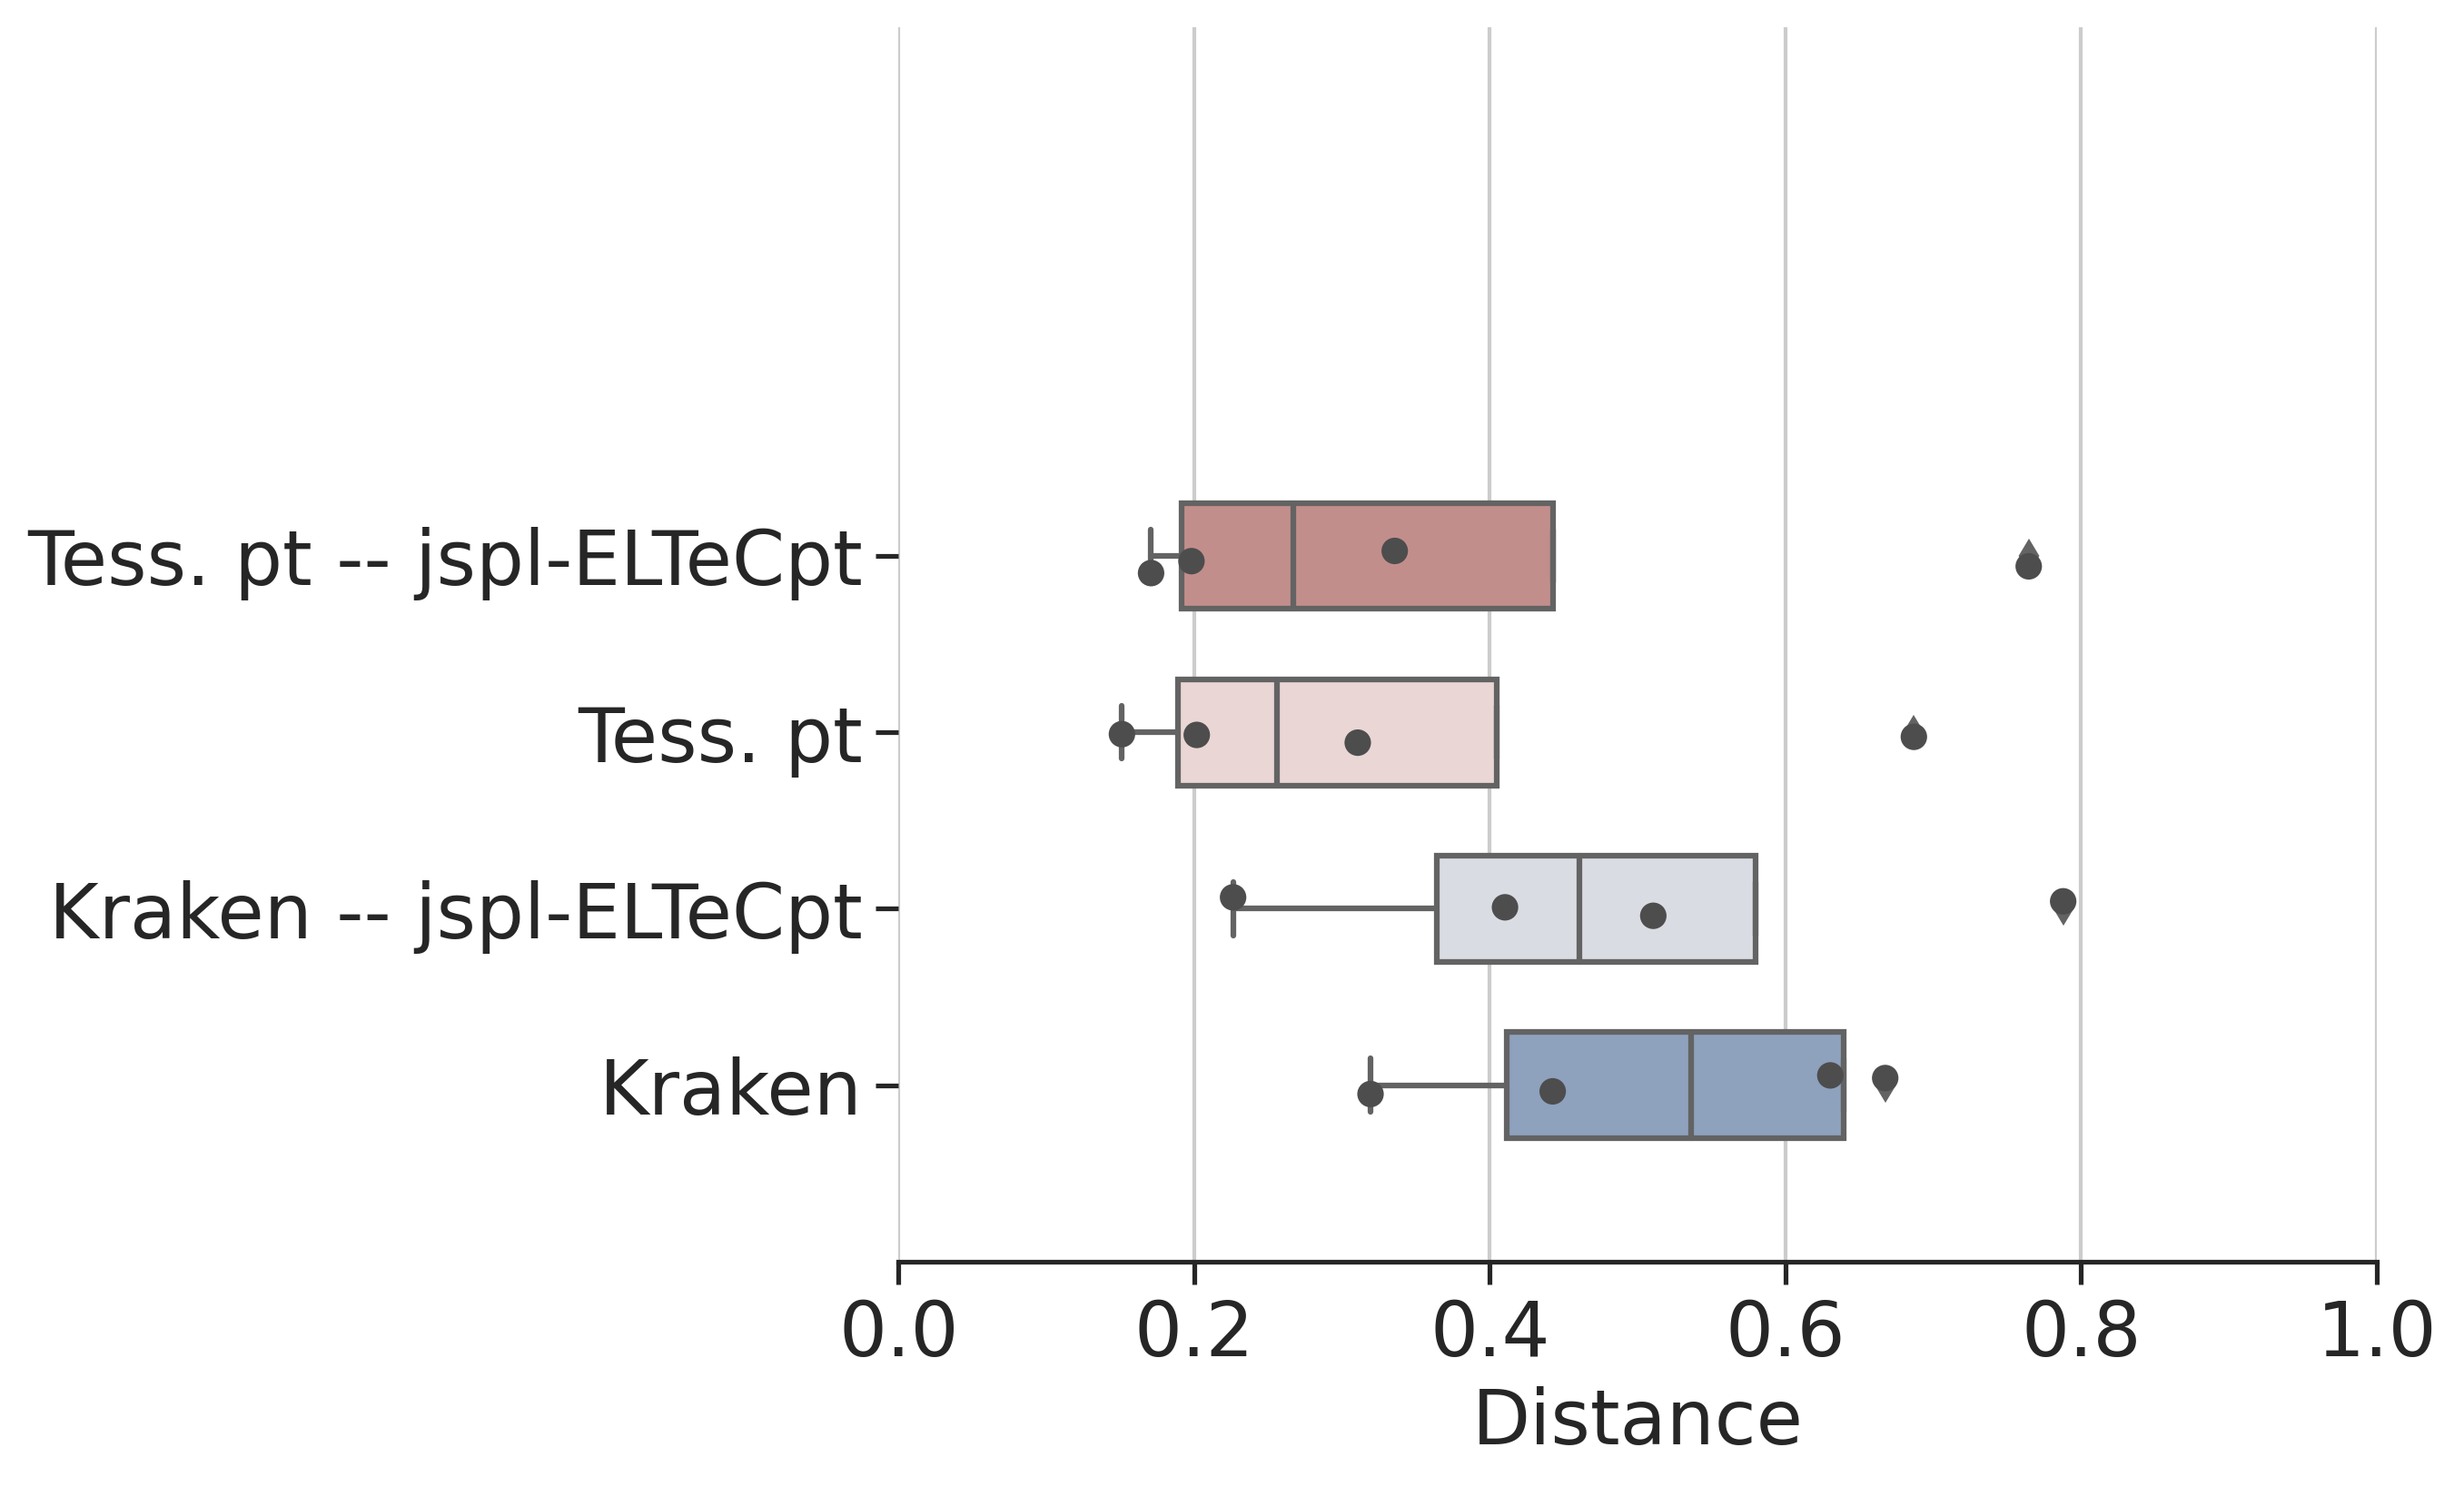
\includegraphics[height=.65\textwidth]{IMAGES/Boite-moustache/ELTeC-Por_spaCy3.5.1_cosinus.png} 
        \caption{ELTeC-Por \texttt{spaCy} cosinus}
   \end{subfigure}
    \caption{Distance Cosinus pour \texttt{spaCy\_lg} et \texttt{stanza} sur chaque sous-corpus globalement.}
    \label{fig:Cosinus-spacy-lg-stanza}
\end{figure}

\subsubsection{\textsc{NERVAL} : Précision, rappel, f-score.}

Dans le but de calculer la précision, le rappel et d'obtenir un f-score nous avons utilisé l'outil \textsc{Nerval}\footnote{\url{https://gitlab.com/teklia/nerval}}, évalué par \cite{koudoro2022reconnaissance}. Si cette évaluation présente quelques biais de l'outil, \textsc{Nerval} apparaît tout de même comme un très bon moyen de dépasser les problèmes d'alignements entre les résultats des différentes configurations à comparer pour calculer le f-score. \textsc{Nerval} est développé en Python, et est conçu pour l'évaluation de sorties de REN sur du texte bruité avec la distance de Levenshtein. Les fichiers des textes de références et des textes versions ROC et ROC corrigées sont annotés au format IOB avec \texttt{spaCy\_lg}\footnote{Le choix de cet outil est déterminé par la multitude des modèles, leurs performances très solides et leur facilité de la prise en main par les chercheur?euses en HN et TAL \cite{DBLP:conf/gis/Koudoro-Parfait21}.}. Les fichiers des textes de références ainsi annotés font office de vérité de terrain.
Les premières observations des résultats semblent confirmer que la correction automatique n'est pas forcément un gain pour la REN, en effet le f-score pour les configurations de Tesseract dans les tableaux \ref{tab:NERVAL_DAUDET} et \ref{tab:NERVAL_THACKERAY} perd en moyenne 0.06 points. À l'inverse, le f-score sur les configurations de Kraken semble légèrement augmenter, ce constat venant illustrer le phénomène de creux que nous évoquions dans la partie \ref{sec:distances_creux}.

\begin{table}[h!]
     \centering
\scriptsize{
\begin{tabular}{|l|r|r|r|r|r|r|}
\hline
 & \multicolumn{2}{c|}{{\# Entités}} & \multicolumn{4}{c|}{\'Evaluation par \textsc{Nerval}}\\
 \hline
Version & ROC & Réf.\ &Intersection& Précision & Rappel & $F_1$ mesure\\

 \hline
Kraken  & 1 122 & 744 &  566  & 0,50    &0,76  &\textit{0,61}  \\
\hline
Tess.fr  & 860 &744  &646     & 0,75     & 0,87  & \textbf{0,81}  \\
\hline
%Tess  & 920  & 944 & 597 & 0.649     & 0.802  & \textit{0.718}  \\
%\hline
\hline
Kraken + Jspll-fr & 1 027  &744  &471     & 0,46     & 0,63  &\textbf{0,53} $\Downarrow$  \\
\hline
Tess.fr + Jspll-fr & 794&  744& 532     & 0,67 & 0,72 & \textit{\textbf{0,69}} $\Downarrow$  \\
\hline
%Tess + Jspllfr &846  & 944 & 503     & 0.595     & 0.676  &\textit{ 0.633 } $\Downarrow$\\
% \hline
\hline
Kraken + ELTeC-fr &1 055 & 744 &548 & 0,52     &0,74  & \textit{0,61} $\Uparrow$ \\
\hline
Tess.fr + ELTeC-fr &838 & 744 & 621  & 0,74     &0,84  & \textit{0,79} $\Downarrow$ \\
%\hline
%Tess + ELTeCfr &927  & 944 &  576    & 0.621     & 0.774  & \textit{0.689} $\Downarrow$\\
\hline
\end{tabular}}
     \caption{Résultat de \textsc{NERVAL} sur {\normalfont Le petit chose}, Daudet.}
     \label{tab:NERVAL_DAUDET}
 \end{table}

   \begin{table}[h!]
     \centering
\resizebox{\textwidth}{!}{
\scriptsize{
\begin{tabular}{|l|l|r|r|r|r|r|r|}
\hline
 & \multicolumn{3}{c|}{{\# Entités}} & \multicolumn{4}{c|}{\'Evaluation par \textsc{Nerval}}\\
 \hline
Version & Label&ROC & Réf.\ &Intersection& Précision & Rappel & $F_1$ mesure\\

 \hline
Kraken  & LOC& 180 & 168&89 &0,50    &0,53 &0,51 \\
Tess. & &161 &168&130&0,81     &0,77&\textbf{0,79} \\
\hline
Kraken &GPE& 1 925 & 1 324& 824&0,43    &0,62 &0,51 \\
Tess. & &1 464 &1 324&1 080&0,74     &0,82&\textbf{0,78} \\
\hline
\hline
Kraken + Jspll-en&LOC & 158 & 168 & 105    &0,67 &0,63&0,64$\Uparrow$ \\ %$\Downarrow$  

Tess. + Jspll-en & & 152&168&119&0,79     &0,71&0,75 $\Downarrow$  
\\
\hline
Kraken  + Jspll-en &GPE&1 542  &1 324&910 &0,59    &0,69 &0,64$\Uparrow$ \\ %$\Downarrow$  

Tess. + Jspll-en  & &1 411 &1 324&1 030&0,73     &0,78&0,75$\Downarrow$ \\
 \hline
\hline
Kraken + ELTeC-en & LOC& 176 &168&99 &0,56    &0,59 &0,58$\Uparrow$\\%$\Uparrow$
Tess. + ELTeC-en& & 158&168&120&0,76     &0,71&0,74 $\Downarrow$\\
\hline
Kraken + ELTeC-en & GPE& 1 149&1 324 &743    &0,65 &0,56 &0,60$\Uparrow$\\%$\Uparrow$

Tess. + ELTeC-en& &1 131 &1 324&868&0,77     &0,66&0,71$\Downarrow$ \\

\hline
\end{tabular}}
}
     \caption{Résultat de \textsc{NERVAL} sur {\normalfont Vanity Fair}, Thackeray.}
     \label{tab:NERVAL_THACKERAY}
 \end{table}



